% Generated fragments require trusted human review before compilation.
% This binder never requests shell escape or runs external tools.
\documentclass[11pt]{article}
% Trusted shared apparatus. Requires LuaLaTeX; never use shell escape.
\usepackage{fontspec}
\defaultfontfeatures{Ligatures=TeX}
\IfFontExistsTF{Noto Serif}{\setmainfont{Noto Serif}}{%
  \IfFontExistsTF{DejaVu Serif}{\setmainfont{DejaVu Serif}}{%
    \IfFontExistsTF{Times New Roman}{\setmainfont{Times New Roman}}{%
      \PackageError{gelfand-binder}{No configured Cyrillic serif font installed}{Install Noto Serif or DejaVu Serif, or select an installed Cyrillic font.}%
    }%
  }%
}
\IfFontExistsTF{Noto Sans}{\setsansfont{Noto Sans}}{%
  \IfFontExistsTF{DejaVu Sans}{\setsansfont{DejaVu Sans}}{\setsansfont{Arial}}%
}
\IfFontExistsTF{Noto Sans Mono}{\setmonofont{Noto Sans Mono}}{%
  \IfFontExistsTF{DejaVu Sans Mono}{\setmonofont{DejaVu Sans Mono}}{\setmonofont{Courier New}}%
}
\usepackage[a4paper,margin=22mm]{geometry}
\usepackage{amsmath,amssymb,amsthm,mathtools}
\usepackage{xcolor}
\usepackage{tikz}
\usepackage{tikz-cd}
\usetikzlibrary{arrows.meta,positioning,calc}
\usepackage{hyperref}
\hypersetup{unicode=true,colorlinks=true,linkcolor=blue,pdftitle={Gelfand transcription binder}}
\newtheorem{theorem}{Theorem}
\newtheorem{lemma}{Lemma}
\newtheorem{proposition}{Proposition}
\newtheorem{corollary}{Corollary}
\theoremstyle{definition}
\newtheorem{definition}{Definition}
\newtheorem{example}{Example}
\theoremstyle{remark}
\newtheorem{remark}{Remark}
\setlength{\parindent}{0pt}
\setlength{\parskip}{0.55em}
\setlength{\emergencystretch}{3em}
\newcommand{\SourcePage}[2]{%
  \clearpage\phantomsection\label{#1:source-page}%
  \addcontentsline{toc}{subsection}{#1}%
  {\small\sffamily\color{blue!60!black}Source scan frame: #1; visible page/leaf label: #2}\par\medskip%
}
\newcommand{\Unclear}[3]{%
  \begingroup\color{orange!70!black}%
  [Unresolved reading #1/#2: #3]\endgroup%
}
\newcommand{\Incomplete}[3]{%
  \par\begingroup\color{red!65!black}\textbf{Incomplete #1/#2:} #3\endgroup\par%
}
\newcommand{\SourceFigure}[3]{%
  \par\begingroup\color{blue!60!black}\textbf{\hyperref[#1:source-page]{Source figure #1/#2}:} #3%
  \par\textit{Consult the authoritative scan at this locator.}\endgroup\par%
}



% Reader layout only. Original diplomatic text is retained verbatim.
\setlength{\parskip}{0.35em}
\setlength{\emergencystretch}{4em}
\renewcommand{\SourcePage}[2]{%
  \par\addvspace{1em}\phantomsection\label{#1:source-page}%
  \addcontentsline{toc}{subsection}{#1}%
  {\footnotesize\sffamily\color{blue!55!black}#1%
    \def\givenlabel{#2}\def\nolabel{unlabelled}%
    \ifx\givenlabel\nolabel\else\quad[номер в источнике: #2]\fi
  }\par\nobreak\smallskip%
}
\renewcommand{\Unclear}[3]{%
  \begingroup\color{orange!65!black}%
  \ifmmode\text{[неясно: #3]}\else[неясно: #3]\fi\endgroup%
}
\renewcommand{\Incomplete}[3]{%
  \par\begingroup\color{red!60!black}\textbf{Неразобранный фрагмент:} #3%
  \endgroup\par%
}
\renewcommand{\SourceFigure}[3]{%
  \par\begingroup\color{blue!55!black}\textbf{Рисунок:} #3%
  \par{\small\textit{Исходный рисунок: \hyperref[#1:source-page]{#1}, #2.}}%
  \endgroup\par%
}
\hypersetup{pdftitle={Семинар И. М. Гельфанда. Дипломатическая транскрипция},pdfauthor={},pdfsubject={Русское рабочее издание с отмеченными сомнительными чтениями}}

\usepackage[normalem]{ulem}
\usepackage{newunicodechar}
\usepackage{adjustbox}
\newfontfamily\SourceSymbolFont{Segoe UI Symbol}
\newfontfamily\SourceCJKFont{MS Gothic}
\let\DiplomaticMathUnderline\underline
\renewcommand{\underline}[1]{\ifmmode\DiplomaticMathUnderline{#1}\else\uline{#1}\fi}
\newunicodechar{→}{\ifmmode\text{{\SourceSymbolFont\char"2192}}\else{\SourceSymbolFont\char"2192}\fi}
\newunicodechar{⇒}{\ifmmode\text{{\SourceSymbolFont\char"21D2}}\else{\SourceSymbolFont\char"21D2}\fi}
\newunicodechar{∀}{\ifmmode\text{{\SourceSymbolFont\char"2200}}\else{\SourceSymbolFont\char"2200}\fi}
\newunicodechar{∂}{\ifmmode\text{{\SourceSymbolFont\char"2202}}\else{\SourceSymbolFont\char"2202}\fi}
\newunicodechar{∈}{\ifmmode\text{{\SourceSymbolFont\char"2208}}\else{\SourceSymbolFont\char"2208}\fi}
\newunicodechar{∌}{\ifmmode\text{{\SourceSymbolFont\char"220C}}\else{\SourceSymbolFont\char"220C}\fi}
\newunicodechar{√}{\ifmmode\text{{\SourceSymbolFont\char"221A}}\else{\SourceSymbolFont\char"221A}\fi}
\newunicodechar{∞}{\ifmmode\text{{\SourceSymbolFont\char"221E}}\else{\SourceSymbolFont\char"221E}\fi}
\newunicodechar{∧}{\ifmmode\text{{\SourceSymbolFont\char"2227}}\else{\SourceSymbolFont\char"2227}\fi}
\newunicodechar{∩}{\ifmmode\text{{\SourceSymbolFont\char"2229}}\else{\SourceSymbolFont\char"2229}\fi}
\newunicodechar{∪}{\ifmmode\text{{\SourceSymbolFont\char"222A}}\else{\SourceSymbolFont\char"222A}\fi}
\newunicodechar{∫}{\ifmmode\text{{\SourceSymbolFont\char"222B}}\else{\SourceSymbolFont\char"222B}\fi}
\newunicodechar{∴}{\ifmmode\text{{\SourceSymbolFont\char"2234}}\else{\SourceSymbolFont\char"2234}\fi}
\newunicodechar{∼}{\ifmmode\text{{\SourceSymbolFont\char"223C}}\else{\SourceSymbolFont\char"223C}\fi}
\newunicodechar{≈}{\ifmmode\text{{\SourceSymbolFont\char"2248}}\else{\SourceSymbolFont\char"2248}\fi}
\newunicodechar{≠}{\ifmmode\text{{\SourceSymbolFont\char"2260}}\else{\SourceSymbolFont\char"2260}\fi}
\newunicodechar{≤}{\ifmmode\text{{\SourceSymbolFont\char"2264}}\else{\SourceSymbolFont\char"2264}\fi}
\newunicodechar{≥}{\ifmmode\text{{\SourceSymbolFont\char"2265}}\else{\SourceSymbolFont\char"2265}\fi}
\newunicodechar{⊕}{\ifmmode\text{{\SourceSymbolFont\char"2295}}\else{\SourceSymbolFont\char"2295}\fi}
\newunicodechar{⊗}{\ifmmode\text{{\SourceSymbolFont\char"2297}}\else{\SourceSymbolFont\char"2297}\fi}
\newunicodechar{①}{\ifmmode\text{{\SourceSymbolFont\char"2460}}\else{\SourceSymbolFont\char"2460}\fi}
\newunicodechar{②}{\ifmmode\text{{\SourceSymbolFont\char"2461}}\else{\SourceSymbolFont\char"2461}\fi}
\newunicodechar{③}{\ifmmode\text{{\SourceSymbolFont\char"2462}}\else{\SourceSymbolFont\char"2462}\fi}
\newunicodechar{④}{\ifmmode\text{{\SourceSymbolFont\char"2463}}\else{\SourceSymbolFont\char"2463}\fi}
\newunicodechar{Ⓗ}{\ifmmode\text{{\SourceSymbolFont\char"24BD}}\else{\SourceSymbolFont\char"24BD}\fi}
\newunicodechar{〃}{\ifmmode\text{{\SourceCJKFont\char"3003}}\else{\SourceCJKFont\char"3003}\fi}


% Reader revision 3. Annotation wording and candidates remain unchanged.
\usetikzlibrary{shapes.geometric,decorations.pathreplacing,decorations.markings,patterns,fit}
\newsavebox{\ReaderAnnotationBox}
\newcommand{\ReaderAnnotation}[1]{%
  \sbox{\ReaderAnnotationBox}{[неясно: #1]}%
  \ifdim\wd\ReaderAnnotationBox>.70\linewidth
    \parbox[t]{.70\linewidth}{\raggedright[неясно: #1]}%
  \else\usebox{\ReaderAnnotationBox}\fi%
}
\ExplSyntaxOn
\cs_new_protected:Npn \reader_unclear_candidate:n #1
 {
  \tl_set:Nx \l_tmpa_tl { \tl_to_str:n {#1} }
  % Text explicitly guarded inside a mathematical candidate remains math-safe.
  \regex_replace_all:nnN { \\(?:text|textrm|textnormal|textbf|operatorname)\s*\{[^{}]*\} } { } \l_tmpa_tl
  \regex_match:nVTF { [\x{0400}-\x{052F}] | \$ } \l_tmpa_tl
   { \ifmmode \text{\ReaderAnnotation{#1}} \else \ReaderAnnotation{#1} \fi }
   {
    \ifmmode
      [\text{неясно:~}#1]
    \else
      \regex_match:nVTF { [_^] | \\ } \l_tmpa_tl
       { \ensuremath{[\text{неясно:~}#1]} }
       { \ReaderAnnotation{#1} }
    \fi
   }
 }
\RenewDocumentCommand \Unclear { m m m }
 { \begingroup\color{orange!65!black}\reader_unclear_candidate:n{#3}\endgroup }
\ExplSyntaxOff
\newsavebox{\ReaderIncompleteBox}
\newcommand{\ReaderIncompleteNote}[1]{%
 \sbox{\ReaderIncompleteBox}{\textbf{Неразобранный фрагмент:} #1}%
 \ifdim\wd\ReaderIncompleteBox>.70\linewidth
  \parbox[t]{.70\linewidth}{\raggedright\textbf{Неразобранный фрагмент:} #1}%
 \else\usebox{\ReaderIncompleteBox}\fi%
}
\renewcommand{\Incomplete}[3]{%
 \ifmmode\text{\color{red!60!black}\ReaderIncompleteNote{#3}}%
 \else\par\begingroup\color{red!60!black}\textbf{Неразобранный фрагмент:} #3\endgroup\par\fi%
}
% Ragged right avoids stretching long untranslated abbreviations into margins.
\AtBeginDocument{\raggedright}
\newunicodechar{А}{\ifmmode\text{\char"410\relax}\else\char"410\relax\fi}
\newunicodechar{Б}{\ifmmode\text{\char"411\relax}\else\char"411\relax\fi}
\newunicodechar{В}{\ifmmode\text{\char"412\relax}\else\char"412\relax\fi}
\newunicodechar{Г}{\ifmmode\text{\char"413\relax}\else\char"413\relax\fi}
\newunicodechar{Д}{\ifmmode\text{\char"414\relax}\else\char"414\relax\fi}
\newunicodechar{Е}{\ifmmode\text{\char"415\relax}\else\char"415\relax\fi}
\newunicodechar{Ж}{\ifmmode\text{\char"416\relax}\else\char"416\relax\fi}
\newunicodechar{З}{\ifmmode\text{\char"417\relax}\else\char"417\relax\fi}
\newunicodechar{И}{\ifmmode\text{\char"418\relax}\else\char"418\relax\fi}
\newunicodechar{Й}{\ifmmode\text{\char"419\relax}\else\char"419\relax\fi}
\newunicodechar{К}{\ifmmode\text{\char"41A\relax}\else\char"41A\relax\fi}
\newunicodechar{Л}{\ifmmode\text{\char"41B\relax}\else\char"41B\relax\fi}
\newunicodechar{М}{\ifmmode\text{\char"41C\relax}\else\char"41C\relax\fi}
\newunicodechar{Н}{\ifmmode\text{\char"41D\relax}\else\char"41D\relax\fi}
\newunicodechar{О}{\ifmmode\text{\char"41E\relax}\else\char"41E\relax\fi}
\newunicodechar{П}{\ifmmode\text{\char"41F\relax}\else\char"41F\relax\fi}
\newunicodechar{Р}{\ifmmode\text{\char"420\relax}\else\char"420\relax\fi}
\newunicodechar{С}{\ifmmode\text{\char"421\relax}\else\char"421\relax\fi}
\newunicodechar{Т}{\ifmmode\text{\char"422\relax}\else\char"422\relax\fi}
\newunicodechar{У}{\ifmmode\text{\char"423\relax}\else\char"423\relax\fi}
\newunicodechar{Ф}{\ifmmode\text{\char"424\relax}\else\char"424\relax\fi}
\newunicodechar{Х}{\ifmmode\text{\char"425\relax}\else\char"425\relax\fi}
\newunicodechar{Ц}{\ifmmode\text{\char"426\relax}\else\char"426\relax\fi}
\newunicodechar{Ч}{\ifmmode\text{\char"427\relax}\else\char"427\relax\fi}
\newunicodechar{Ш}{\ifmmode\text{\char"428\relax}\else\char"428\relax\fi}
\newunicodechar{Щ}{\ifmmode\text{\char"429\relax}\else\char"429\relax\fi}
\newunicodechar{Ъ}{\ifmmode\text{\char"42A\relax}\else\char"42A\relax\fi}
\newunicodechar{Ы}{\ifmmode\text{\char"42B\relax}\else\char"42B\relax\fi}
\newunicodechar{Ь}{\ifmmode\text{\char"42C\relax}\else\char"42C\relax\fi}
\newunicodechar{Э}{\ifmmode\text{\char"42D\relax}\else\char"42D\relax\fi}
\newunicodechar{Ю}{\ifmmode\text{\char"42E\relax}\else\char"42E\relax\fi}
\newunicodechar{Я}{\ifmmode\text{\char"42F\relax}\else\char"42F\relax\fi}
\newunicodechar{а}{\ifmmode\text{\char"430\relax}\else\char"430\relax\fi}
\newunicodechar{б}{\ifmmode\text{\char"431\relax}\else\char"431\relax\fi}
\newunicodechar{в}{\ifmmode\text{\char"432\relax}\else\char"432\relax\fi}
\newunicodechar{г}{\ifmmode\text{\char"433\relax}\else\char"433\relax\fi}
\newunicodechar{д}{\ifmmode\text{\char"434\relax}\else\char"434\relax\fi}
\newunicodechar{е}{\ifmmode\text{\char"435\relax}\else\char"435\relax\fi}
\newunicodechar{ж}{\ifmmode\text{\char"436\relax}\else\char"436\relax\fi}
\newunicodechar{з}{\ifmmode\text{\char"437\relax}\else\char"437\relax\fi}
\newunicodechar{и}{\ifmmode\text{\char"438\relax}\else\char"438\relax\fi}
\newunicodechar{й}{\ifmmode\text{\char"439\relax}\else\char"439\relax\fi}
\newunicodechar{к}{\ifmmode\text{\char"43A\relax}\else\char"43A\relax\fi}
\newunicodechar{л}{\ifmmode\text{\char"43B\relax}\else\char"43B\relax\fi}
\newunicodechar{м}{\ifmmode\text{\char"43C\relax}\else\char"43C\relax\fi}
\newunicodechar{н}{\ifmmode\text{\char"43D\relax}\else\char"43D\relax\fi}
\newunicodechar{о}{\ifmmode\text{\char"43E\relax}\else\char"43E\relax\fi}
\newunicodechar{п}{\ifmmode\text{\char"43F\relax}\else\char"43F\relax\fi}
\newunicodechar{р}{\ifmmode\text{\char"440\relax}\else\char"440\relax\fi}
\newunicodechar{с}{\ifmmode\text{\char"441\relax}\else\char"441\relax\fi}
\newunicodechar{т}{\ifmmode\text{\char"442\relax}\else\char"442\relax\fi}
\newunicodechar{у}{\ifmmode\text{\char"443\relax}\else\char"443\relax\fi}
\newunicodechar{ф}{\ifmmode\text{\char"444\relax}\else\char"444\relax\fi}
\newunicodechar{х}{\ifmmode\text{\char"445\relax}\else\char"445\relax\fi}
\newunicodechar{ц}{\ifmmode\text{\char"446\relax}\else\char"446\relax\fi}
\newunicodechar{ч}{\ifmmode\text{\char"447\relax}\else\char"447\relax\fi}
\newunicodechar{ш}{\ifmmode\text{\char"448\relax}\else\char"448\relax\fi}
\newunicodechar{щ}{\ifmmode\text{\char"449\relax}\else\char"449\relax\fi}
\newunicodechar{ъ}{\ifmmode\text{\char"44A\relax}\else\char"44A\relax\fi}
\newunicodechar{ы}{\ifmmode\text{\char"44B\relax}\else\char"44B\relax\fi}
\newunicodechar{ь}{\ifmmode\text{\char"44C\relax}\else\char"44C\relax\fi}
\newunicodechar{э}{\ifmmode\text{\char"44D\relax}\else\char"44D\relax\fi}
\newunicodechar{ю}{\ifmmode\text{\char"44E\relax}\else\char"44E\relax\fi}
\newunicodechar{я}{\ifmmode\text{\char"44F\relax}\else\char"44F\relax\fi}
\newunicodechar{Ё}{\ifmmode\text{\char"401\relax}\else\char"401\relax\fi}
\newunicodechar{ё}{\ifmmode\text{\char"451\relax}\else\char"451\relax\fi}


% Reader-only pairing support; accepted raw bodies remain unchanged.
\RequirePackage{graphicx}
\RequirePackage{adjustbox}
\newcommand{\ReaderOriginalPanel}[2]{%
  \begin{minipage}[t]{.48\linewidth}\vspace{0pt}\centering
    \includegraphics[width=\linewidth,keepaspectratio]{#1}\par\smallskip
    {\scriptsize Оригинал рукописного рисунка: #2}\par
  \end{minipage}%
}
\newcommand{\ReaderDiagramPair}[3]{%
  \par\noindent\begingroup
  \ReaderOriginalPanel{#1}{#2}\hfill
  \begin{minipage}[t]{.48\linewidth}\vspace{0pt}\centering
    {\scriptsize Типографское воссоздание}\par\smallskip
    \begin{adjustbox}{max width=\linewidth}#3\end{adjustbox}\par
  \end{minipage}%
  \endgroup\par\smallskip
}
\newcommand{\ReaderDescriptionPair}[3]{%
  \par\noindent\begingroup
  \ReaderOriginalPanel{#1}{#2}\hfill
  \begin{minipage}[t]{.48\linewidth}\vspace{0pt}\raggedright
    {\scriptsize Типографское описание}\par\smallskip
    #3\par
  \end{minipage}%
  \endgroup\par\smallskip
}


\begin{document}
\begin{center}
{\Large Семинар И. М. Гельфанда}\par\medskip
{\LARGE Дипломатическая транскрипция}\par\bigskip
{\large Рабочее русское издание}\par\medskip
{\large Том 16 из 34. Архивная глава 016}\par\bigskip
Кадры GELFAND-P000848 -- GELFAND-P000899\par
\end{center}
\medskip
Сокращения, отменённые записи и сомнительные чтения сохранены.
Неразобранные фрагменты отмечены в тексте. Математические утверждения
источника переданы без молчаливых исправлений.

В текущем комплекте приняты 165 из 165 возвратов; учтены 1527 из 1527 кадров. Кадров без принятого возврата: 0.
Статусы кадров в отчётах о полноте: транскрибированы 1168, неразборчивы 357, частично прочитаны 1, недоступны 1.
Нерешённых записей журнала чтений: 6820.
Статус «неразборчивый» может отмечать локальную утрату зачёркнутой записи;
он не означает отсутствия всего кадра.
Сверка с рукописью продолжается. Рабочие журналы чтений и происхождения
данных сохранены отдельно.

Ограничения исходного комплекта: повреждённый исходный скан GELFAND-P000722; каталожные записи 603, 694 без сканов; в архивной главе 029 не перечислена часть 25.

Границы кадров показаны небольшими синими указателями; печатный текст
продолжается без обязательного разрыва страницы после каждого кадра.
\bigskip\hrule\bigskip
\SourcePage{GELFAND-P000848}{1}
% Оригинал 2440 x 3480; координаты обзора в пикселях от левого верхнего угла.
% Верх: (40,75)-(2130,717), просмотр оригинала и увеличений 3x, 5x, 6x.
\underline{1.10.79} \qquad \underline{Сем. Гельфанда}

[Зачёркнутый заголовок: \Unclear{GELFAND-P000848}{top-cancelled-heading}{КАЛЛОШ?}]

\underline{И. М. Г.} Что такое спинор?

\underline{Книга Паули по \Unclear{GELFAND-P000848}{book-abbreviation}{квант.} мех.} — самое хорошее излож. теории Дирака (ур-е Дирака)

Возражения его против теор. Дирака:

а) сущ. \underline{позитронов}, предсказ. теор. Дирака.

б) если они есть, то при столкн. с \Unclear{GELFAND-P000848}{annihilation-word}{позитр.} получ. 2 фотона

в) 2 фотона по этой теории могут родить пару \Unclear{GELFAND-P000848}{pair-abbreviation}{эл-н/позитрон}

% Рассказ о Дираке: (150,734)-(1790,1041), 3x и 6x; зачёркивание 8x.
Дирак \Unclear{GELFAND-P000848}{dirac-abbreviation}{отказ.}, чтобы не сделали „сэром“ (?)

[Следующие строки объединены скобкой слева:]
\begin{quote}
Однажды ему кто-то сказал, что не понимает ф-лу в левом нижнем углу доски.

Дирак не отвечает.

Председатель просит его ответить

[Зачёркнуто: \Unclear{GELFAND-P000848}{anecdote-cancelled-word}{неразборчиво}.]
Дирак: „не было вопроса, было утверждение“.
\end{quote}

% Гамильтон: (240,1027)-(2150,1685), 3x; последний знак 10x, тёмный штрих 8x.
\underline{Гамильтон}: хотел извлечь корень из $x^2+y^2+z^2$, причем получить „лин. форму“
\begin{equation*}
-(x^2+y^2+z^2)=(ax+by+cz)^2
\end{equation*}
\begin{equation*}
a^2=b^2=c^2=\Unclear{GELFAND-P000848}{hamilton-square-sign}{-1}
\end{equation*}
\begin{equation*}
(ab+ba)\Unclear{GELFAND-P000848}{hamilton-factor-mark}{?}xy
+(ac+ca)xz+(bc+cb)yz+a^2x^2+b^2y^2+c^2z^2=-(x^2+y^2+z^2).
\end{equation*}
отсюда соотношения
\begin{equation*}
ab+ba=0 \quad \text{и т. д.}
\end{equation*}
Добавл. единицу — получ. \underline{кватернионы}.

Рассм. преобразование
\begin{equation*}
z'=\frac{az+b}{cz+d}
\end{equation*}
% Однородные координаты: (375,1774)-(1570,2032), 3x.
или
\begin{equation*}
\begin{cases}
z'_1=az_1+bz_2\\
z'_2=cz_1+dz_2
\end{cases}
\qquad z'=\frac{z'_1}{z'_2},\quad z=\frac{z_1}{z_2}.
\end{equation*}

% Определение и рекомендация: (193,2040)-(1650,2463), 3x.
Спиноры — пара чисел [Под словом «чисел»: «(компл.)»], преобр. по такому закону

Компл. сопр. — \underline{сопр.} \underline{спинор.}

\underline{Гравитацию} надо читать по Ландау и Лифшицу (т. 2)

\underline{гл. 1, 2, 10, 11.}

% Программа: (150,2520)-(2320,3360), 3x; последняя строка 5x.
\underline{Рената Э. Каллош.}

\underline{Программа.}

1. Двухкомпонентные спиноры.

2. Самодуальность.

3. Дифф. оператор $\Delta(A,B)$, описыв. ур-е для частиц высш. спинов.

4. Ур-е теплопров., нулевые и ненулевые моды.

5. Теоремы об индексе.

6. Супертеор. в гравит. п-ле

7. Суперсамодуальность.

(8. Супертеор. об индексе! Её \Unclear{GELFAND-P000848}{program-last-verb}{записал} Зингер, но на самом деле её нет.)

\SourcePage{GELFAND-P000849}{unlabelled}
% Original frame: 2440 x 3480 pixels. Main column and right-margin notes retained.
\underline{Лит-ра}

1. [Зачёркнуто: \Unclear{GELFAND-P000849}{bibliography-first-cancelled}{неразборчиво}.]
\underline{S. W. Hawking}, \underline{C. N. Pope}

Nucl. Phys., B 146 (\Unclear{GELFAND-P000849}{bibliography-first-year}{1978 / 1971}), 381

2. \underline{Р. Э. Каллош}, Письма в ЖЭТФ,

\underline{29} (1979), 192; 493

3. S. M. Christensen, M. J. Duff.

Nucl. Phys. (1979), 301

4. — ” —, — ” — Deser, \Unclear{GELFAND-P000849}{bibliography-fourth-last-author}{Cu / Ci}

Phys Lett. \underline{84 B} (1979), 411

[1] — осн. вклад в супергравит. (в 1-петлевом прибл.) — от $0^{\underline{\text{х}}}$ мод

(в Я.-М. — от всех мод!)

[2], [3] незав. — в суперграв. (для самодуальн.) для более высоких порядков

Перед этим \Unclear{GELFAND-P000849}{before-supergravity}{был / было} в 1-м и 2-м пор. суперг. не сод. расход.

[3] осн. на обычной теор. об индексе.

\underline{2-комп. формализм Ван-дер-Вардена.}

Закон преобразований
\begin{equation*}
\Psi_\alpha\longrightarrow\Psi_\beta\Omega_\alpha^\beta \tag{1}
\end{equation*}

[На правом поле:]
$\Psi_\alpha\in(\text{\Unclear{GELFAND-P000849}{margin-representation-abbreviation}{пр. / ир.} станд. 2-мерн. пр. }SL(2,C))=V;$

$\Psi_{\dot\alpha}\in\bar V$, $V\otimes\bar V$ имеет вещ. стр.

и гр. $SL(2,C)$ сохр.

кв. форму.

(гр. Лор. у Пенроуза)

$SL(2,C)$ как

\Unclear{GELFAND-P000849}{margin-real-lie}{вещ. мн. Ли / вещ. гр. Ли}

\SourceFigure{GELFAND-P000849}{margin-stepped-bracket}{Ступенчатая линия под заметкой о $\bar V$: вправо, вниз, вправо, вниз; ниже продолжается вертикальная линия слева от слов «$SL(2,C)$ как». Точное отнесение ответвлений к соседним строкам не установлено.}

[Основной текст:]
Если гр. Лоренца или $SO(4)$
\begin{equation*}
\Omega_\alpha^\beta=(\omega^{ab}\Sigma_{ab})_\alpha^\beta \tag{2}
\end{equation*}
$\alpha,\beta=1,2.$

(закон преобр. 2-х комп. спинора)

$\Sigma_{ab}$ — фиксир. матрицы (вроде матр. Паули) 2-го порядка

$\omega^{ab}$ — параметры

Для матриц Паули
\begin{equation*}
\text{\Unclear{GELFAND-P000849}{pauli-product-source}{$\sigma_i\sigma_j=\delta_{ij}+\epsilon_{ijk}\sigma^k$}} \tag{3}
\end{equation*}
\begin{equation*}
\sigma^a=(I,i\vec\sigma);\qquad a=1,2,3,4.
\end{equation*}
\begin{equation*}
\Sigma_{ab}=\sigma_a\bar\sigma_b-\bar\sigma_b\sigma_a \tag{4}
\end{equation*}

Теперь о величинах в спинорных обозначениях.

\underline{Пенроуз} сформулировал так теорию гравитации.

Пусть есть вектор $x_a$; тогда
\begin{equation*}
X_{\alpha\dot\alpha}=\sigma^a_{\alpha\dot\alpha}x_a\quad\text{— спинор} \tag{5}
\end{equation*}
\begin{equation*}
\Psi_{\alpha_1\ldots\alpha_{2A},\dot\alpha_{\text{\Unclear{GELFAND-P000849}{equation-six-first-dotted-index}{2 / 1}}}\ldots\dot\alpha_{2B}}=\Psi(A,B) \tag{6}
\end{equation*}

\SourcePage{GELFAND-P000850}{2}
% Original frame: 2440 x 3480 pixels. The visible page label is 2.
и если произвести полную симметризацию, то получим неприв. представление.

Кстати о матрицах Паули: они таковы.
\begin{equation*}
\left\{\begin{aligned}
\sigma^1_{\alpha\dot\alpha}&=\frac{1}{\sqrt2}\begin{pmatrix}0&1\\1&0\end{pmatrix};\\
\sigma^2_{\alpha\dot\alpha}&=\frac{1}{\sqrt2}\begin{pmatrix}0&-i\\i&0\end{pmatrix};\\
\sigma^3_{\alpha\dot\alpha}&=\frac{1}{\sqrt2}\begin{pmatrix}1&0\\0&-1\end{pmatrix};\\
\sigma^4_{\alpha\dot\alpha}&=\frac{1}{\sqrt2}\begin{pmatrix}1&0\\0&1\end{pmatrix}.
\end{aligned}\right. \tag{7}
\end{equation*}
[Первый нижний индекс в $\sigma^1$ переписан поверх прежнего знака: \Unclear{GELFAND-P000850}{pauli-first-index-overwritten}{прежний знак неразборчив; сверху читается $\alpha$}.]

Есть ещё $\epsilon^{\alpha\beta}$
\begin{equation*}
\epsilon^{12}=1;\qquad\epsilon_{\alpha\beta}=\begin{bmatrix}0&1\\-1&0\end{bmatrix} \tag{8}
\end{equation*}

Опускание индексов:
\begin{equation*}
\Psi_\alpha=\epsilon_{\alpha\beta}\Psi^\beta \tag{9}
\end{equation*}

\underline{И. М. Г.}

По коорд. $\dot\alpha$ преобр. комплексно сопряженное.

\tikz{\node[draw,circle,inner sep=2pt]{!};}
Ф-ла (5) — \underline{констр. спинора по вектору}

\begin{center}— · —\end{center}

\underline{К.} Рассм. [Зачёркнуто: \Unclear{GELFAND-P000850}{before-antisymmetric-cancelled}{неразборчиво}.] теперь антисимметр. тензоры

\begin{equation*}
\begin{aligned}
F_{[ab]}\longmapsto F_{\alpha\dot\beta\gamma\dot\delta}
&=\epsilon_{\alpha\gamma}F_{\dot\beta\dot\delta}+\epsilon_{\dot\beta\dot\delta}F_{\alpha\gamma},
\end{aligned} \tag{10}
\end{equation*}
[Под $F_{[ab]}$:] антисимм. тензор

(это только для антисимм.)

— легко проверить

[Справа:] $F_{\alpha\gamma},F_{\dot\beta\dot\delta}$ — симм. тензоры

[На правом поле:]
\begin{equation*}
\Lambda^2(S\otimes\bar S)=\Lambda^2S\otimes S^2\bar S+S^2S\otimes\Lambda^2\bar S \tag{*}
\end{equation*}
соб. знач. опер. $*$ — $\pm1$

\underline{Самодуальный тензор:} опр. опер. $*$:
\begin{equation*}
{}^*F_{ab}=\frac12\epsilon_{abcd}F^{cd} \tag{11}
\end{equation*}

\underline{самодуальность:}
\begin{equation*}
F_{ab}=\pm{}^*F_{ab};\quad
\text{[Зачёркнуто: \Unclear{GELFAND-P000850}{selfduality-cancelled}{неразборчиво}.]}
\quad\{F_{\alpha\beta}=0\quad\text{или}\quad F_{\dot\alpha\dot\beta}=0\} \tag{12}
\end{equation*}

\underline{О гравитации}

\underline{Тензор кривизны:} $R_{abcd}$. Считается, что есть метрика

и определение операции $*$:
\begin{equation*}
{}^*R_{abcd}=\frac12\epsilon_{ab}{}^{c'd'}R_{c'd'cd} \tag{13}
\end{equation*}
[Правее формулы — бледные остатки записи: \Unclear{GELFAND-P000850}{curvature-faint-trailing}{неразборчиво}.]

Спинорный эквивалент. Ур-я Эйнш. вытек. из усл. самодуальности

(и поэтому много гравит. инстантонов)
\begin{equation*}
R_{\alpha\beta\gamma\delta}\quad\text{и}\quad R_{\dot\alpha\dot\beta\dot\gamma\dot\delta}
\end{equation*}
\begin{equation*}
R_+=R+{}^*R=0\quad\text{— см. ур-е $(*)$}.
\end{equation*}

[Справа, за скобкой:] см. лекц. Хокинга, 1978 г. со ссылкой на Пенроуза

\begin{equation*}
\Phi(A,B)=\Psi_{\alpha_1,\ldots,\alpha_{2A},\dot\alpha_1,\ldots,\dot\alpha_{2B}} \tag{14}
\end{equation*}

Ур-я сод. кучу разных ур-й — Максвелл, де Вит, Швингер, Эйнштейн,

Ходж — де Рам (для дифф. форм).

(см. [3])

\SourcePage{GELFAND-P000851}{unlabelled}
% Original frame: 2440 x 3480 pixels.
Спинор пока симметр. (соотв. неприв. предст.). Определим $\Delta$.
\begin{equation*}
\begin{aligned}
(\Delta\Phi)_{\alpha_1\ldots\alpha_{2A},\dot\alpha_1\ldots\dot\alpha_{2B}}
={}&\bigl(-\Box\epsilon_{\alpha_1\beta}
+2\nabla_{\dot\xi(\alpha_1}\nabla_{\beta)}^{\dot\xi}\bigr)
\bar\Phi^\beta{}_{\alpha_2\ldots\alpha_{2A},\dot\alpha_1\ldots\dot\alpha_{2B}}.
\end{aligned} \tag{15}
\end{equation*}

\underline{Свойства.}
\begin{equation*}
1)\qquad (\Phi,\Delta\Phi)=(\Delta\Phi,\Phi) \tag{16}
\end{equation*}
\begin{equation*}
2)\qquad \Delta\Phi(0,0)=-\Box\Phi,\qquad\text{здесь}\quad
\Box=\nabla_{\alpha\dot\alpha}\nabla^{\alpha\dot\alpha}, \tag{17}
\end{equation*}
\begin{equation*}
\nabla_{\alpha\dot\alpha}=\sigma^a_{\alpha\dot\alpha}D_a;\qquad D_a=\partial_a+B_a
\end{equation*}

3) Дирак $\Phi(1/2,0)$ (в кривом пр-ве)
\begin{equation*}
\Psi_\pm=(1\pm\gamma_5)\Psi \tag{18}
\end{equation*}
$\Psi$ — 4-компон. Дираковский спинор
\begin{equation*}
\Delta\Psi_\pm=\left(-\Box+\frac14R\right)\Psi_\pm
\end{equation*}
[Под $R$:] скал. кривизна

4) Максвелл в \Unclear{GELFAND-P000851}{maxwell-gauge-abbreviation}{лорн. / лор.} калибровке
\begin{equation*}
\Delta A_a=(-\Box g_{ab}+R_{ab})A^b,\qquad
\text{\Unclear{GELFAND-P000851}{maxwell-overwritten-operator}{$D$ / $\nabla$}}^a A_a=0 \tag{19}
\end{equation*}
[Оператор перед $A_a$ переписан поверх другого знака; отдельные слои записи не разделяются.]

\begin{equation*}
5)\qquad\underline{s=\frac32}\qquad\text{кого то и Швингера} \tag{20}
\end{equation*}
\begin{equation*}
6)\quad\underline{s=2}\quad\text{Эйнштейн} \tag{21}
\end{equation*}
\begin{equation*}
7)\qquad\omega=\frac1{p!}\omega_{\mu_1\ldots\mu_p}dx^{\mu_1}\wedge\ldots\wedge dx^{\mu_p} \tag{22}
\end{equation*}
\begin{equation*}
\Phi(0,0),\quad\Phi(1/2,1/2),\quad\Phi(1,0),\quad\Phi(0,1)
\end{equation*}
\begin{equation*}
\Delta=\delta d+d\delta
\end{equation*}

[Зачёркнутый знак перед строкой: \Unclear{GELFAND-P000851}{before-standard-cancelled}{неразборчиво}.]
Станд. теория дифф. форм опис. \underline{\underline{бозоны}}.

Если бы были нечётные — то вся мат.

[3] — на форму повесили чётные инд.

\underline{Надо:} сделать антикоммутирующие $dx$.

[Справа:] Березин частично сделал.

Пока нет [Зачёркнуто: \Incomplete{GELFAND-P000851}{after-poka-cancelled}{два зачёркнутых слова не удалось прочитать}.]

дифф. форм, сод. среди $dx$ \underline{комм. и антикоммут.}

ввести оператор $\Delta$ и построить \underline{теор. индекса}

Бозонное поле $\Psi_a$ даёт форму $\Psi_a dx^a$.

Для спина $\frac52$ все ур-я не годятся (не удаётся сделать взаимодействие)

— ” — $\frac32$ только что сделано (супергравитация)

\underline{Идея И. М. Г.} возможно, не обязательно $d\delta+\delta d$.

\SourcePage{GELFAND-P000852}{3}
% Original frame inspected at 2440 x 3480 pixels. Coordinates below are original-image pixels, origin upper left.
Эквивалентная форма записи $\Delta$:
\begin{equation*}
\Delta=-\Box+X,\tag{23}
\end{equation*}
\begin{equation*}
X=-\Sigma^{ab}R_{ab}^{cd}\Sigma_{cd},\qquad A+B\text{ — целое}\tag{24}
\end{equation*}
\begin{equation*}
X=-\frac{1}{A}\Sigma^{ab}R_{+ab}^{cd}\Sigma_{cd},\qquad A+B\text{ — полуцелое},\quad A>B.\tag{25}
\end{equation*}
% Interlinear addition at [741,462,1054,583], with an upward arrow pointing to R in (25).
\textit{[Вставка со стрелкой к $R$ в (25):]} $(R_+=R+{}^{*}R)$

$\varphi$ здесь симметрична по $\alpha_1\ldots\alpha_{2A}$ и по $\dot\alpha_1\ldots\dot\alpha_{2B}$.
\begin{equation*}
\Delta\varphi=\lambda\varphi\tag{26}
\end{equation*}
Отсюда будет следовать условие совместности.
% Circled interlinear insertion and crossed-out duplicate number: [128,730,1480,901].
\textit{[Вставка в овале:]} (и из симметрии)
\textit{[Зачёркнуто: (26); от зачёркнутой строки проведена стрелка к вставке.]}

\underline{Условие совместности:}
\Unclear{GELFAND-P000852}{equation27-number}{номер формулы: (27) или (28), последняя цифра переправлена}
\begin{equation*}
\nabla_{\dot\alpha}^{(\alpha_1}\nabla^{\alpha_2)\dot\alpha}
\varphi_{\alpha_1\alpha_2\ldots\alpha_{2A},\dot\alpha_1\ldots\dot\alpha_{2B}}=0
\end{equation*}
$A\leq1$, $B\leq1$ $\Rightarrow$ случай всех физ. полей

Рассм. ур-е теплопроводности
\begin{equation*}
\frac{d}{dt}F(x,x',t)+\Delta F(x,x',t)=0,\qquad
F\big|_{t=0}=\delta(x-x').\tag{28}
\end{equation*}
на компактном мн-зии
\begin{equation*}
\operatorname{Tr}F(x,x,t)\underset{t\to+0}{\sim}
\sum_{k=0}^{\infty}b_k t^{(k-4)/2}\tag{29}
\end{equation*}
[\Unclear{GELFAND-P000852}{equation29-coefficient-edit}{между $b_k$ и $t$ — переправленные мелкие знаки; возможно, зачёркнутое $(x)$}]
[\Unclear{GELFAND-P000852}{equation29-exponent-deletion}{перед сохранившимся показателем $(k-4)/2$ зачёркнута прежняя запись; неразборчиво}]
\begin{equation*}
B_k=\int d^4x\sqrt{g}\,b_k,\tag{30}
\end{equation*}
Тогда
\begin{equation*}
B_4=n+m.\tag{31}
\end{equation*}
$B_4$ — первый нерасходящийся.

$n$ — число 0-х соб. значений (26)

$m$ — \textit{[зачёркнуто: число ненулевых соб. знач.]}
\textit{[Вписано под зачёркнутым:]} кратность ненулевого (любого) соб. знач.

\textit{[Справа:]} [их общая кратность — все кратности одинаковы!!]
— гипотеза С. Гиндикина
\textit{[Под этой записью, со стрелкой вверх:]} \underline{наверно.}

Цель — выраз. через топ. инварианты.

\underline{Gilkey} дошел до
\Unclear{GELFAND-P000852}{gilkey-coefficient}{$b_6$ или $B_6$, буква переправлена}.
(1975)
\textit{[Под коэффициентом:]} 1979
\Unclear{GELFAND-P000852}{gilkey-year-word}{есть или ещё}
(И.М.Г.)
\textit{[Под годом (1975):]} ссылка здесь
\Unclear{GELFAND-P000852}{gilkey-reference-word}{точная или такая}

Если есть граница, то тоже $b_4$ сейчас
[\Unclear{GELFAND-P000852}{boundary-deleted-word}{зачёркнутое слово; неразборчиво}]
недавно написано; вопрос счит. сложным.

Рассм. приводимые предст.
\begin{equation*}
\varphi_{\alpha\beta}=\varphi_{(\alpha\beta)}+
\frac{1}{2}\varepsilon_{\alpha\beta}\varphi_{\alpha}^{\alpha}\tag{32}
\end{equation*}
\begin{equation*}
[1,0]=(1,0)\oplus(0,0)
\end{equation*}
В силу условий совместности
\begin{equation*}
[\nabla_{\alpha}^{\dot\alpha},\Delta]\varphi[A,B]=0\tag{33}
\end{equation*}

\SourcePage{GELFAND-P000853}{unlabelled}
% Original frame inspected at 2440 x 3480 pixels. Coordinates below are original-image pixels, origin upper left.
\begin{equation*}
(\Delta-\lambda)\varphi_{\alpha_1\ldots}=0\tag{34}
\end{equation*}
Рассм.
\begin{equation*}
\Psi_{\alpha_1\ldots\alpha_{2A-1}\dot\alpha_1\ldots\dot\alpha_{2B+1}}
=\nabla_{\dot\alpha_{2B+1}}^{\alpha_{2A}}
\varphi_{\alpha_1\ldots\alpha_{2A}\dot\alpha_1\ldots\dot\alpha_{2B}}\tag{35}
\end{equation*}
$\Psi\ne0$ при $\varphi\ne0$ (иначе
\Unclear{GELFAND-P000853}{after35-symbol}{крест с малым овалом сверху; возможно $\overset{\circ}{\times}$}
с (34)).
\begin{equation*}
m[A,B]=m[A-\tfrac{1}{2},B+\tfrac{1}{2}]\tag{36}
\end{equation*}
\textit{[Под $m$, с выносной чертой:]} число ненулев. мод
\begin{equation*}
A+B=S,\qquad A-B=T.
\end{equation*}
Тогда получим
\begin{equation*}
m[S,T]=m[S]\tag{37}
\end{equation*}
Отсюда
\begin{equation*}
n[S,T]-n[S,T']=B_4[S,T]-B_4[S,T']\tag{38}
\end{equation*}
\begin{equation*}
n[S,T]-n[S,T-1]=4^{S-1}\bigl((T-\tfrac{1}{2})\chi+(S-\tfrac{2}{3})\tfrac{p}{2}\bigr)\tag{39}
\end{equation*}
$\chi$ — число Эйлера, $p$ — число Понтрягина

\underline{Об ур-и теплопров.}
\begin{equation*}
F(x,x',t)=\sum_{i=0}^{\infty}\varphi_i(x)\varphi_i(x')e^{-\lambda_i t}\tag{40}
\end{equation*}
$\varphi_i$ — ортонорм. сист.
\begin{equation*}
F(x,x',0)=\delta(x,x')\tag{41}
\end{equation*}
\begin{equation*}
\int_M d^4x\sqrt{g}\,F(x,x,t)
=\sum_{i=0}^{\infty}e^{-\lambda_i t}
=n+\sum_{i=n+1}^{\infty}e^{-\lambda_i t}\tag{42}
\end{equation*}
[\Unclear{GELFAND-P000853}{equation42-deleted-mark}{над вторым $x$ в $F$ зачернён небольшой знак; возможно, зачёркнутый штрих}]
\begin{equation*}
F(x,x,t)\sim\sum_{k=0}^{\infty}b_k(x)t^{\Unclear{GELFAND-P000853}{equation43-exponent}{(k-4/2}}\tag{43}
\end{equation*}
\textit{[После переправленной цифры 4 самостоятельная закрывающая скобка неразличима.]}

$m$ опред. отсюда!! — выкидыванием расх. членов
$\sum e^{-\lambda_i t}$ и \underline{даёт вклад}.

\underline{$m$ — регуляриз. сумма}

«$m$ — целое (!) из глубоких топ. соображений»

Это станд. однопетлевые расх. контин. интегралы.
% The abbreviation and isolated letter were independently cross-reviewed at 4x.
\textit{[Правее, на той же строке, отдельно:]} в

Опред. $\chi$ и $p$ для мн-зии без края
\begin{equation*}
\chi=\int {}^{*}R_{abcd}\,{}^{*}R^{abcd}\,d^4x\sqrt{g}\tag{44}
\end{equation*}
\begin{equation*}
p=\int {}^{*}R_{abcd}R^{abcd}\,d^4x\sqrt{g}\tag{45}
\end{equation*}

\SourcePage{GELFAND-P000854}{4}
% Original frame inspected at 2440 x 3480 pixels. Coordinates in the ledger are original-image pixels, origin upper left.
\underline{8.10.79.} \underline{Сем. Гельфанда.}

\underline{Проект теор. минимума}, \underline{необх. при любой специализации}. (для 1-курсников)

1. \underline{Алгебра}

Ван дер Варден, гл. 1–5, 12.

Гельфанд Лекции по лин. алгебре

Атья, Макдональд

2. \underline{Анализ}
\begin{equation*}
\underline{\text{или}}\quad
\left\{\begin{array}{l}
\text{Берс}\\
\text{[зачёркнуто: }\Unclear{GELFAND-P000854}{analysis-cancelled-name}{фамилия, возможно Берман}\text{] Лузин}\\
\text{Берман}
\end{array}\right\}\quad\text{для втузов}
\end{equation*}
потом.
\begin{equation*}
\text{или}\quad
\left\{\begin{array}{l}
\text{Рудин}\\
\text{Дьедонне}\\
\text{Грауэрт, Либ, Фишер}\\
\text{Шварц}
\end{array}\right\}
\qquad
\begin{array}{l}
\text{Спивак}\\
\text{Бишоп - Криттенден}\\
\text{Номидзу}
\end{array}
\end{equation*}

\underline{Контр. вопрос:} вычислить приблизительно
\begin{align*}
&\int_{-\infty}^{\infty}e^{-x^2}\cos1000x\,dx,\qquad
\int_{-\infty}^{\infty}e^{-1000x^2}\cos x\,dx
\qquad\text{(и сравн. с табл.)}\\
&\int_{-\infty}^{\infty}e^{-1000x^4}\cos x\,dx,\qquad
\int_{-\infty}^{\infty}e^{-x^4}\cos1000x\,dx
\end{align*}

3. \underline{Арнольд} $\mathrm{I},\ \mathrm{II},\ \mathrm{III}.$

4. \underline{Кириллов} $\frac{1}{2}+\frac{1}{2}$

\underline{Серр} лин. предст. конечных групп

(3-ю главу он не понимает)

\underline{Обобщ. ф-и} $\mathrm{I}$ вып., главы 1–2

5. \underline{Знать ур-я в частных производных.} (читать некого).

\textit{[Две строки подчёркнуты волнистой линией:]}

Контр. зад. по лин. алгебре:

найти кан. форму самосопр. опер. в
[\Unclear{GELFAND-P000854}{symplectic-deleted-word}{зачёркнутое слово; неразборчиво}]
симплект. пр-ве.

6. [\Unclear{GELFAND-P000854}{reading6-blackened-mark}{зачернённый одиночный знак перед «Спец.»; возможно, буква А}]
\underline{Спец. теория отн. $+$ ОТО}

$+$ \underline{геометрия}

\textit{[Справа от пункта 6:]}
Ландау, Лифшиц (т. 2)

\Unclear{GELFAND-P000854}{nomizu-note-abbreviation}{связ. или свяж.}
с Номидзу

\bigskip
\underline{\underline{С. Гиндикин.}} \underline{Начала теории твисторов.}

Будет рассказ. на языке интегр. геометрии.

\textit{[Справа:]}
Твисторы ввёл \underline{Пенроуз}.

см. один из посл. номеров BAMS,

1979, т. 1 (нов. серия),

ст. \underline{Уэллса} (\underline{Wells})

[\Incomplete{GELFAND-P000854}{cancelled-before-diagram}{Зачёркнутая строка перед диаграммой не прочитана; последнее слово, возможно, «пространство»}]
\begin{equation*}
\begin{adjustbox}{max width=\linewidth}
\begin{tikzcd}
\mathbb{C}^{4}\setminus0 \arrow[d]\\
\mathbb{C}P^{3}
\end{tikzcd}
\end{adjustbox}\tag{1}
\end{equation*}

В $\mathbb{C}^{4}$ фиксируем эрмитову форму
[\Unclear{GELFAND-P000854}{hermitian-blackened-symbol}{зачернённый знак перед скобкой; неразборчиво}]
$(++--)$. $\langle\ ,\ \rangle$.

Получаются $\alpha$-твисторы: элементы $\mathbb{C}P^3$ или соотв. элем. $\mathbb{C}^4$.

$(\mathbb{C}P^3)'$ — двойств. пр-во. Там тоже возник. форма и это — $\beta$-твисторы.

\SourcePage{GELFAND-P000855}{unlabelled}
\begin{align*}
\langle z,z\rangle>0&\Rightarrow\text{полож. твистор}\\
\langle z,z\rangle=0&\Rightarrow\text{нулевой — ″ —}\\
\langle z,z\rangle<0&\Rightarrow\text{отриц. — ″ —}
\end{align*}
В $\mathbb{C}P^3$ рассм. прямые (2-мерн. подпр. в $\mathbb{C}^4$).
Их мн-во: $G=G_{4,2}=G_{4,2}^{\mathbb{C}}$.
Над $G$ есть \Unclear{GELFAND-P000855}{bundle-word}{естественное}
рассл. 2-реперов (главное) в $\mathbb{C}^4$:
\begin{equation*}
\begin{adjustbox}{max width=\linewidth}
\begin{tikzcd}[row sep=small]
E\arrow[d]\\
G
\end{tikzcd}
\end{adjustbox}
\tag{2}
\end{equation*}
[Над заголовком зачёркнута строка: \Incomplete{GELFAND-P000855}{cancelled-heading-line}{Полное чтение зачёркнутой строки не установлено: буквы закрыты многочисленными штрихами.}]
[Слева от заголовка зачёркнуто: \Unclear{GELFAND-P000855}{cancelled-heading-prefix}{неразборчиво}.]

\underline{Координаты в $G$.}

Выберем в $\mathbb{C}^4$ 2 плоскости (трансверс.) $L$ и $L'$, тогда любая другая — график,
матрица соотв. преобр. — координаты.
[В предыдущей строке «$L$ и $L'$» вставлено над строкой со знаком вставки.]
Выб. в [Зачёркнуто: \Unclear{GELFAND-P000855}{cancelled-before-l}{неразборчиво}.]
$L$ базис $e_0\ e_1$; в $L'$ базис $e_3,e_4$.
Тогда если $\widetilde L\in G_{4,2}$, то в $\widetilde L$ есть базис вида
\begin{equation*}
\begin{cases}
f_0=e_0+u_{03}e_3+u_{04}e_4\\
f_1=e_1+u_{\Unclear{GELFAND-P000855}{formula-3-index}{1}3}e_3+u_{14}e_4
\end{cases}
\tag{3}
\end{equation*}
$u_{ij}$ — координаты.

Пусть $L,L'$ трансверс. и изотропные относит. $\langle\cdot,\cdot\rangle$.
\underline{Задача.} Такие $L$ и $L'$ существуют.
\begin{equation*}
\{e_A,\ A=0,1\}\text{ — базис в }L.
\tag{4}
\end{equation*}
В $L'$ введ. базис
\begin{equation*}
\{e^{A'},\ A'=0',1'\}\text{ — базис в }L'
\tag{5}
\end{equation*}
[Перед словом «форма» над строкой вставлено «Пусть»; после слова «форма» над строкой вставлены знаки $\langle\ ,\ \rangle$.]
[Зачёркнуто: \Unclear{GELFAND-P000855}{cancelled-form-prefix}{неразборчиво}.]
Пусть [Зачёркнуто: \Unclear{GELFAND-P000855}{cancelled-after-pust}{неразборчиво}.]
форма $\langle\ ,\ \rangle$ в базисе $(e_0,e_1,e^{0'},e^{1'})$ имеет
[Зачёркнуто: \Unclear{GELFAND-P000855}{cancelled-before-matrix}{неразборчиво}.] матрицу
\begin{equation*}
\begin{pmatrix}0&iE\\-iE&0\end{pmatrix};
\tag{6}
\end{equation*}
т. е.
\begin{equation*}
\langle e_0,e^{0'}\rangle=\langle e_1,e^{1'}\rangle=i,
\qquad\text{остальные скал. произв.}=0
\tag{7}
\end{equation*}
Сделаем замену переменных в $L$:
\begin{equation*}
\widetilde e_B=g_B^A e_A
\tag{8}
\end{equation*}
Тогда легко проверить, что
\begin{equation*}
e^{A'}\text{ преобр. с помощью }(g^*)^{-1}
\tag{9}
\end{equation*}
(выводится из соотн. [Зачёркнуто: \Unclear{GELFAND-P000855}{cancelled-orthogonality-word}{неразборчиво}.] ортогональности)

Есть и другие законы преобр.:
[Слева зачёркнуто: \Unclear{GELFAND-P000855}{cancelled-index-intro}{неразборчиво}.]
\begin{equation*}
\begin{array}{ll}
A'\quad\text{с пом. }\bar g&B'\quad\text{с пом. }(g^*)^{-1}\\
B\quad\text{— ″ — }(g^T)^{-1}&
\end{array}
\end{equation*}
\SourceFigure{GELFAND-P000855}{index-transformation-arcs}{Над и слева от $A'$ проходит дуга; под и слева от $B$ и $B'$ проходят дуги. Видимые буквы и формулы переданы выше; точное значение и способ передачи дуг не установлены.}

\SourcePage{GELFAND-P000856}{5}
\underline{Задача.} Доказать, что в $U(2,2)$ есть подгруппа, изом. $GL(2,\mathbb{C})$
(указ. воспольз. предыдущим).

Координаты:
\begin{equation*}
\{z^A,z_{A'}\}\qquad\text{по базису }\{e_A,e^{A'}\}
\tag{10}
\end{equation*}
\begin{equation*}
z=z^Ae_A+z_{A'}e^{A'}\in\mathbb{C}^4
\tag{11}
\end{equation*}
\underline{\underline{И.М.Г.}} $\mathbb{C}^4\ni(x_1,x_2,x_3,x_4)$
\begin{equation*}
\langle x,y\rangle=x_1\bar y_1+x_2\bar y_2
\Unclear{GELFAND-P000856}{formula-12-sign}{-}
x_3\bar y_3-x_4\bar y_4
\tag{12}
\end{equation*}
$L,L'$ — 2 изотропных подпр-ва и 2 базиса $\{e_0,e_1\}$; $\{e^{0'},e^{1'}\}$.
Тогда
\begin{equation*}
z=z^0e_0+z^1e_1+z_{0'}e^{0'}+z_{1'}e^{1'}
\tag{13}
\end{equation*}
\begin{equation*}
\{z^A,z_{A'}\}\text{ — спинорные координаты в }\mathbb{C}^4
\tag{14}
\end{equation*}
Требование на базис:
\begin{equation*}
\langle e_0,e^{0'}\rangle=\langle e_1,e^{1'}\rangle=i,
\qquad\text{остальные скал. произв.}=0.
\tag{15}
\end{equation*}
\underline{\underline{С.Г.}} Пусть
$\widetilde L\in G$; $\widetilde L\cap L'=\{0\}$.
Тогда выб. базис так:
\begin{equation*}
f_A=e_A+u_{AB'}e^{B'}
\tag{16}
\end{equation*}
Спинорные индексы сами показывают как они преобразуются.
(полезно выписать!)

(Теория твисторов в кривом пространстве пока не сделана, хотя уже есть работы).
Рассм. группы, действ. в $\mathbb{C}^4$.
действ. $GL(4,\mathbb{C})$ переносится в $G_{4,2}$.
\begin{align*}
T_+&:\quad\langle z,z\rangle>0\\
T_-&:\quad\langle z,z\rangle<0\\
N&:\quad\langle z,z\rangle=0\qquad\text{— 7-мерная пов. в }\mathbb{C}^4.
\end{align*}
\begin{align*}
S_+&\text{ — 2-мерные плоск. }\subset T_+\quad\text{(кроме 0)}\\
S_-&\text{ — — ″ — }\subset T_-\quad\text{(— ″ —)}\\
M&\text{ — — ″ — }\subset N
\end{align*}
$S_+,S_-$ — лежат целиком в пределах действия коорд. $u_{AB'}$.
\begin{equation*}
\begin{cases}
S_+=\{u:\ \frac{1}{i}(u-u^*)\gg0\}\\
S_-=\{u:\ \frac{1}{i}(u-u^*)\ll0\}
\end{cases}
\tag{17}
\end{equation*}

\SourcePage{GELFAND-P000857}{unlabelled}
$M$ уже не лежит целиком в коорд. окрестности.
Пусть $M_0$ — та часть к-рая лежит.
\begin{equation*}
M_0=\{u:\ u=u^*\}
\tag{18}
\end{equation*}
\begin{equation*}
\dim_{\mathbb{R}}M_0=4,\qquad\dim_{\mathbb{C}}S^{\pm}=4.
\end{equation*}
$M_0$ — общий остов $S^{\pm}$.
\begin{equation*}
\partial S_+=\{\text{опорные плоскости к }T_+\}
\end{equation*}
Рассм. теперь в $\mathbb{C}^4$ группу $U(2,2)$, сохр.
[Зачёркнуто: \Unclear{GELFAND-P000857}{cancelled-before-form}{неразборчиво}.] форму
(и, следов., поверхность $N$). Тогда ясно, что $U(2,2)$ сохр. все
[Зачёркнуто: \Unclear{GELFAND-P000857}{cancelled-before-domains}{неразборчиво}.]
области $S_{\pm},M$ (канонич. конструкция) и действует на каждой \underline{транзитивно}!!
(\underline{Задача из лин. алгебры!})

На $(\mathbb{C}^4,\langle\ ,\ \rangle)$ действует $U(2,2)$ и сохр. всю конструкцию.
$g\in U(2,2)$ записываем в базисе опис. выше вида:
\begin{equation*}
g=\begin{pmatrix}A&B\\C&D\end{pmatrix}
\tag{19}
\end{equation*}
\underline{Действие на $u$:}
\begin{equation*}
g:\ u\mapsto(Au+B)(Cu+D)^{-1}
\tag{20}
\end{equation*}
Действие превр. $M$ в конформную компактификацию пр-ва Минковского:
гр. Пуанкаре $\subset SU(2,2)$ (добавл. конформных преобр.).

% A short vertical annotation stroke is drawn beneath G_0 in the source.
\begin{center}
\begin{adjustbox}{max width=\linewidth}
\begin{tikzpicture}
\node at (0,0) {$G$};
\node at (0.65,0) {$\supset$};
\node at (1.35,0) {$G_0$};
\draw (1.35,-0.23)--(1.35,-0.48);
\node[anchor=north west] at (0.95,-0.52) {плоск., трансверс. $L'$};
\end{tikzpicture}
\end{adjustbox}
\end{center}
Рассм. подгруппу, сохр. $G_0$ ($\sim$ сохр. $L'$).
Эта группа изом. \Unclear{GELFAND-P000857}{poincare-group-source}{гр. Пуанкаре}:
\begin{equation*}
u\to aua^*+b
\tag{21}
\end{equation*}
$a\in GL(2,\mathbb{C})$, $b=b^*$.

В записи (19) здесь:
\begin{equation*}
A=a,\quad C=0,\quad D=(a^*)^{-1},\quad BD^{-1}=b.
\tag{22}
\end{equation*}
\begin{equation*}
\text{Метрика Минковского на }M_0^{\Unclear{GELFAND-P000857}{formula-23-superscript}{4}}:
\qquad\det(du)
\tag{23}
\end{equation*}
Коорд. Паули (на $M_0$):
\begin{equation*}
\begin{pmatrix}
u_0-u_1&u_3+i u_4\\
u_3-i u_4&u_1+u_0
\end{pmatrix},\qquad u_j\in\mathbb{R}
\tag{24}
\end{equation*}
% GELFAND-0092. Дипломатическая транскрипция исходных скан-кадров.
% Координаты в примечаниях и журнале: пиксели исходника 2440 x 3480,
% начало в левом верхнем углу; прямоугольники (x0,y0,x1,y1).
\SourcePage{GELFAND-P000858}{6}
% REVIEW: исходные пиксели 2440 x 3480; (x0,y0,x1,y1), начало слева сверху.
% REVIEW top: 70,20,2250,480; увеличение 1x.
% REVIEW middle: 250,480,1800,1250; увеличение 1x.
% REVIEW lower: 230,1230,2100,1710; увеличение 1x.
% REVIEW metric: 1000,130,1140,205; увеличение 5x.
% REVIEW coordinate-note: 800,365,1200,467; увеличение 3x.
% REVIEW cancellation: 300,950,600,1040; увеличение 3x.
% REVIEW flag: 760,1570,930,1670; увеличение 3x.
Тогда метрика принимает вид
\begin{equation*}
(du_0)^2-(du_1)^2-(du_2)^2-(du_3)^3. \tag{25}
\end{equation*}
\Unclear{GELFAND-P000858}{metric-power}{Показатель последнего слагаемого: $3$ [так в источнике].}
\begin{equation*}
M_0=M\cap G_0\underset{\mathrm{def}}{=}\text{обычное пр-во Минковского}. \tag{26}
\end{equation*}
[Под $G_0$, с выносной чертой: коорд. окрестность.]

Точка $M$ --- это точка $G$ или прямая в $\mathbb{C}P^3$.
Ограничимся рассмотрением $M_0$.

\begin{adjustbox}{max width=\linewidth}
\begin{tikzpicture}
\draw (0,0) -- (2,1.2);
\node[right] at (2,1.2) {$l_0$};
\end{tikzpicture}
\end{adjustbox}

Рассм. все прямые, пересек. с $l_0$.
Ур-е для них в координатах:
\begin{equation*}
\det(u^0-u)=0. \tag{27}
\end{equation*}
Оказывается, что это
[Зачёркнуто: \Unclear{GELFAND-P000858}{cancelled-word}{неразборчиво}.]
конус изотропии Минковского
(конус нулевых лучей).
\begin{equation*}
(27)\cap M=\{\text{световой конус}\}.
\end{equation*}
Имеется вз.-однозн. соотв. между точками $M$ и лучами на $N$.
\begin{equation*}
\text{Световые лучи на }M=\text{точки в }\mathbb{C}P^3.
\end{equation*}
[Над «точки» вставлено с выносным знаком: изотропные.]

\underline{Конкурс}: сформулировать многомерное обобщение этой ситуации.
\begin{equation*}
\text{прямая}\rightsquigarrow\text{флаг}.
\end{equation*}
\begin{center}--- $\cdot$ ---\end{center}

\SourcePage{GELFAND-P000859}{unlabelled}
% REVIEW: исходные пиксели 2440 x 3480; (x0,y0,x1,y1), начало слева сверху.
% REVIEW lower-first: 180,2200,1900,2900; увеличение 1x.
% REVIEW lower-last: 210,2870,2260,3480; увеличение 1x.
% REVIEW parity: 520,2650,835,2830; увеличение 3x.
\underline{\underline{15.10.79.}} \quad \underline{Сем. Гельфанда.}

\underline{\underline{Ф.А. Березин.}} \quad \underline{Суперматематика.}

$\mathbb{K}$ --- поле ($\mathbb{R}$ или $\mathbb{C}$).

$\mathbb{Z}_2$-град. пр-во $L=L_0\oplus L_1$.

Элементы $L_0$ и $L_1$ наз. однородными.

Чётность
\begin{equation*}
\alpha(x)=\begin{cases}0,&x\in L_0,\\1,&x\in L_1.\end{cases}
\end{equation*}
Суммы и произв. понимаются $\bmod 2$.

Грассм. алгебра $\Lambda$ на $\mathbb{K}$ --- ассоц. алг. с образующими
\begin{equation*}
1\ (\in\mathbb{K}),\quad \xi_1,\ldots,\xi_N
\end{equation*}
и соотнош.
\begin{equation*}
\xi_i\xi_j+\xi_j\xi_i=0,\quad\forall i,j.
\end{equation*}
\begin{equation*}
\{1,\ \xi_{i_1}\ldots\xi_{i_k},\ i_1<i_2<\ldots<i_k\}
\quad\text{--- базис в }\Lambda\text{ над }\mathbb{K}.
\end{equation*}
$\Lambda=\Lambda_0\oplus\Lambda_1$, \quad
$\Lambda_0$ порожд. $1$ и произв. чётного числа $\xi_i$.

\SourcePage{GELFAND-P000860}{10}
% REVIEW: исходные пиксели 2440 x 3480; (x0,y0,x1,y1), начало слева сверху.
% REVIEW upper: 90,0,2240,870; увеличение 1x.
% REVIEW middle-upper: 120,865,2230,1680; увеличение 1x.
% REVIEW middle-lower: 90,1620,2240,2500; увеличение 1x.
% REVIEW lower: 100,2500,2250,3380; увеличение 1x.
% REVIEW cancelled-definition: 115,435,960,555; увеличение 3x.
% REVIEW envelope-subscript: 400,1050,1060,1200; увеличение 3x.
% REVIEW grading-cancellation: 330,2330,440,2480; увеличение 4x.
% REVIEW even-block-indices: 960,3100,1230,3210; увеличение 5x.
% REVIEW diagram: 370,1620,1450,1760; увеличение 3x.
\begin{equation*}
\dim_{\mathbb{K}}\Lambda=2^N.
\end{equation*}
Для однородных $f,g$
\begin{equation*}
f\cdot g=(-1)^{\alpha(f)\cdot\alpha(g)}gf. \tag{1}
\end{equation*}
Грассманова оболочка лин. пр-ва $L$:

[Зачёркнута строка: \Unclear{GELFAND-P000860}{cancelled-definition}{$(2)$? $L(\Lambda)=L\otimes_{\mathbb{K}}\Lambda$?}]

$e_i$ --- базис в $L$ из однор. элементов
$(L=L_0\oplus L_1)$.

Рассм. теперь
\begin{equation*}
\left\{\sum a_i e_i,\ a_i\in\Lambda,\ \alpha(a_i)=\alpha(e_i)\right\}
\underset{\mathrm{def}}{=}L(\Lambda). \tag{2}
\end{equation*}
\underline{Это левый $\Lambda_0$-модуль.} Иначе:
\begin{equation*}
L(\Lambda)=(\Lambda\otimes_{\mathbb{K}}L)_{\bar 0}. \tag{2'}
\end{equation*}
Линейные операторы.

\underline{И.М.Г.} Алг. эти возникают в теории предст. колчанов.
(ср. ФА, 1979, $N=3$).

\underline{Гип.}: $\forall$ схеме Дынкина должен быть аналог
\underline{чётной части гр. алгебры}.
(так что обычная соотв. схеме $A_n$

\SourceFigure{GELFAND-P000860}{dynkin-chain}{Семь кружков вдоль почти горизонтальной линии, соединённых последовательно; явных наконечников стрелок нет. Над первым кружком $e_1e_2$ или $e_i e_2$, над вторым $e_2e_3$, над третьим $e_3e_4$, над последним $e_{n-1}e_n$. Индекс первой подписи требует проверки.}

если соед. стрелкой, то произв. $=0$, если не соед., то новый элемент.
Идея: есть алг. типа Грассмана, но другие.
\begin{center}--- $\cdot$ ---\end{center}

оператор в $L$:
\begin{equation*}
A=\begin{pmatrix}A_{11}&A_{12}\\A_{21}&A_{22}\end{pmatrix}. \tag{3}
\end{equation*}
Градуировка:

[Перед первой матрицей зачёркнут знак:
\Unclear{GELFAND-P000860}{grading-cancellation}{$A$?}]
\begin{equation*}
\underset{\text{0-я комп.}}{\begin{pmatrix}A_{11}&0\\0&A_{22}\end{pmatrix}}
\qquad
\underset{\text{1-я комп.}}{\begin{pmatrix}0&A_{12}\\A_{21}&0\end{pmatrix}}. \tag{4}
\end{equation*}
Пр-во $L_{p,q}$ --- все такие опер., $p=\dim L_0$, $q=\dim L_1$.

$L_{p,q}(\Lambda)$ --- грассм. оболочка.

\underline{Замечание}: $a_i$ и $e_i$ всегда счит. коммутирующими.

$L_{p,q}(\Lambda)$ --- тоже матрицы из грассм. чисел:

в \Unclear{GELFAND-P000860}{even-block-indices}{$A_{11},A_{22}$?} чётные

в $A_{12},A_{21}$ нечётные.

\SourcePage{GELFAND-P000861}{unlabelled}
% REVIEW: исходные пиксели 2440 x 3480; (x0,y0,x1,y1), начало слева сверху.
% REVIEW upper: 160,0,2290,1050; увеличение 1x.
% REVIEW middle: 230,1040,2330,2100; увеличение 1x.
% REVIEW lower: 170,2100,2340,3480; увеличение 1x.
% REVIEW product-symbols: 550,1080,1390,1220; увеличение 3x.
% REVIEW cancelled-word: 1320,905,1460,987; увеличение 4x.
% REVIEW post-matrix-mark: 1410,1670,1530,1790; увеличение 4x.
% REVIEW faded-fragment: 390,2240,640,2340; увеличение 3x.
% REVIEW projection: 600,2500,2170,2650; увеличение 3x.
% REVIEW final-diagonal: 680,3270,1340,3420; увеличение 3x.
\begin{equation*}
A=\begin{pmatrix}A_{11}&A_{12}\\A_{21}&A_{22}\end{pmatrix}\in L_{p,q}(\Lambda).
\end{equation*}
$L_{p,q}(\Lambda)$ --- \underline{это алгебра} (и $\Lambda_0$-модуль).

Суперслед
\begin{equation*}
\operatorname{str} A=\operatorname{tr} A_{11}-\operatorname{tr} A_{22}. \tag{5}
\end{equation*}
Св-во:
\begin{equation*}
\operatorname{str}(AB)=\operatorname{str}(BA). \tag{6}
\end{equation*}
\underline{Супердетерминант} (Березиниан):
\begin{equation*}
\operatorname{sdet}=\det(A_{11}-A_{12}A_{22}^{-1}A_{21})(\det A_{22})^{-1}. \tag{7}
\end{equation*}
(для числовых матриц есть ф-ла
[Зачёркнуто: \Unclear{GELFAND-P000861}{cancelled-word}{неразборчиво}.]
такая же, но с $\det A_{22}$ вместо $(\det A_{22})^{-1}$).
\begin{equation*}
\operatorname{sdet}(\alpha_1\alpha_2)=\operatorname{sdet}\alpha_1\cdot\operatorname{sdet}\alpha_2. \tag{8}
\end{equation*}
\Unclear{GELFAND-P000861}{product-symbols}{Обозначения в (8): $\alpha_1,\alpha_2$ или рукописные $A_1,A_2$.}

\underline{Упражнение}. Сделать это, если $\dim L_0=\dim L_1=1$,
т.е. для матриц 2-го порядка.

\underline{Пояснение}. Рассм. матрицы с антикоммут. элементами:
\begin{equation*}
\operatorname{sdet}\begin{pmatrix}1&\xi_1\\\xi_2&1\end{pmatrix}=1-\xi_1\xi_2.
\end{equation*}
\begin{equation*}
\begin{pmatrix}1&\xi_1\\\xi_2&1\end{pmatrix}^{2}
=\begin{pmatrix}1+\xi_1\xi_2&2\xi_1\\2\xi_2&1+\xi_2\xi_1\end{pmatrix}.
\end{equation*}
[Справа от матрицы: \Unclear{GELFAND-P000861}{post-matrix-mark}{знак, похожий на \#; возможно, зачёркивание}.]
\begin{align*}
\operatorname{sdet}
&=(1+\xi_1\xi_2-2\xi_1(1+\xi_1\xi_2)2\xi_2)(1+\xi_1\xi_2)=\\
&=(1-3\xi_1\xi_2)(1+\xi_1\xi_2)=1-2\xi_1\xi_2=(1-\xi_1\xi_2)^2.
\end{align*}
\underline{Привед. матриц к кан. виду.}

\Unclear{GELFAND-P000861}{faded-fragment}{$L(\Lambda)$?}

Имеется отображение
\begin{equation*}
m.\quad L(\Lambda)\longrightarrow L_0
\end{equation*}
\begin{equation*}
\sum a_i e_i\longmapsto\left.\left(\sum a_i e_i\right)\right|_{\xi=0}
=\sum m(a_i)e_i,\qquad m(a_i)=\left.a_i\right|_{\xi=0}.
\end{equation*}
[Под последним знаком суммы зачёркнут индекс:
\Unclear{GELFAND-P000861}{cancelled-sum-index}{неразборчиво}.]
\begin{equation*}
A=\begin{pmatrix}A_{11}&A_{12}\\A_{21}&A_{22}\end{pmatrix}\in L_{p,q}(\Lambda).
\end{equation*}
\begin{equation*}
m(A)=\begin{pmatrix}a_1&0\\0&a_2\end{pmatrix}. \tag{9}
\end{equation*}
Пусть $\mathbb{K}=\mathbb{C}$.

\underline{Теорема}.
Пусть $m(A)$ имеет разл. соб. знач. Тогда $A$ тоже прив.
к диаг. виду:
\begin{equation*}
BAB^{-1}=\begin{pmatrix}c_1&&0\\&\ddots&\\0&&c_{p+q}\end{pmatrix}. \tag{10}
\end{equation*}

\SourcePage{GELFAND-P000862}{11}
% REVIEW: исходные пиксели 2440 x 3480; (x0,y0,x1,y1), начало слева сверху.
% REVIEW upper: 125,0,2320,960; увеличение 1x.
% REVIEW middle: 115,940,2350,2030; увеличение 1x.
% REVIEW lower: 155,2020,2350,3470; увеличение 1x.
% REVIEW speaker: 205,2310,565,2420; увеличение 3x.
% REVIEW theorem-name: 250,2430,1040,2550; увеличение 3x.
% REVIEW cancelled-qualifier: 1820,3110,1930,3200; увеличение 4x.
% REVIEW references: 320,970,1730,1150; увеличение 3x.
% REVIEW graded-chain: 400,1370,1690,1525; увеличение 3x.
\underline{Аналоги жорд. клеток здесь неизвестны.}

\underline{Задача 1}. \underline{Сделать это} (\underline{аналог норм. форм})!

Задача, имеющая отношение к инстантонам:

\underline{Задача 2}. Рассм. матрицу $A=(a_{ik})_{i,k=1}^{n}$ с элементами
$a_{ik}\in\Lambda_1$ (неч. гр. числа).

Описать все $B=(b_{ik})_{i,k=1}^{n}$, с элем. $b_{ik}\in\Lambda_0$
и такие что
\begin{equation*}
\underline{\underline{AB=BA}}.
\end{equation*}
Если $\Lambda$ имеет 4 образующих, то имеет отн. к Я.-М.

Если все элем. $A$ независимы (в $\Lambda$), то решается.
\begin{center}--- $\cdot$ ---\end{center}

\underline{\underline{С.Г.}} Связь с раб. Бейлинсона и Берншт.-Гельф.-Гельф.

(см. ФА, 1978, $N=3$?; или Дринфельд, Манин; Яд. физика, $N=6$, 1979:
там явно указ. констр., перев. на язык решений).

\underline{классиф. вект. рассл.} на $\mathbb{C}P^3$. (голом.)

Объекты --- град. модули над $\Lambda=\Lambda(4)$:
\begin{center}
\begin{adjustbox}{max width=\linewidth}
\begin{tikzcd}[column sep=small]
V_{-N}\arrow[r,"\xi_\alpha"] & V_{-N+1}\arrow[r] & \ldots\arrow[r] & V_{-1}\arrow[r] & V_0\arrow[r] & V_1\arrow[r] & V_2
\end{tikzcd}
\end{adjustbox}
\end{center}
$\alpha=1,2,3,4$. \quad Предст. грассм. алгебры:
\begin{equation*}
\xi_i\xi_j+\xi_j\xi_i=0.
\end{equation*}
$a_1\xi_1+a_2\xi_2+a_3\xi_3+a_4\xi_4$ --- оператор из $V_k$ в $V_{k+1}$

и получ. \underline{комплекс};

когом. нулевые, кроме $H^0$.

Такие модули с точн. до экв. классифицируют инстантоны.

\underline{Задача}: дать явную конструкцию. Не сделано (строятся пр-ва, но
не отображения).

\underline{Задача}: \underline{сделать классиф. для грассманова мн-зия}!!

\underline{\underline{Ю. Шабат.}}
\Unclear{GELFAND-P000862}{speaker-initial}{Инициал «Ю.» [так в источнике].}

\underline{Теорема Ли--Виртингера} (классическая)

$\Gamma\subset\mathbb{C}^{n}$ --- росток аналитич. гиперповерхности.
Она наз. \underline{двойной пов. переноса}, если она 2-мя спос. предст.
в виде суммы
\begin{equation*}
\Gamma=\gamma_1+\ldots+\gamma_{n-1},
\end{equation*}
\begin{equation*}
\Gamma=\delta_1+\ldots+\delta_{n-1}
\end{equation*}
$\gamma_i,\delta_i$ --- ростки аналит. кривых

$\{\gamma_i\}$ и $\{\delta_i\}$ не получ. друг из друга перест.
[Зачёркнуто: \Unclear{GELFAND-P000862}{cancelled-qualifier}{неразборчиво}.]
и сдвигами.

\underline{Пример}: $X$ --- гладкая кривая рода $n$.

$JX$ --- якобиан кривой $X$; \quad $j:X\longrightarrow JX$.

\SourcePage{GELFAND-P000863}{unlabelled}
% REVIEW: исходные пиксели 2440 x 3480; (x0,y0,x1,y1), начало слева сверху.
% REVIEW upper: 250,0,2340,1125; увеличение 1x.
% REVIEW middle: 170,1110,2270,2310; увеличение 1x.
% REVIEW lower: 110,2310,2250,3470; увеличение 1x.
% REVIEW riemann-constant: 610,280,1620,495; увеличение 3x.
% REVIEW hypothesis-word: 1200,1250,1620,1370; увеличение 3x.
% REVIEW name: 195,1410,640,1560; увеличение 3x.
% REVIEW map-symbol: 160,1980,300,2120; увеличение 4x.
% REVIEW cancelled-form-prefix: 200,2340,330,2420; увеличение 4x.
% REVIEW cancelled-star: 925,2580,1100,2700; увеличение 5x.
% REVIEW hypothesis-word-wide: 1080,1230,1450,1360; увеличение 3x.
% REVIEW embedded-curve: 350,790,1780,920; увеличение 3x.
\begin{equation*}
\Theta=\underbrace{j(X)+\ldots+j(X)}_{n-1\text{ раз}},
\qquad (\Theta\text{-дивизор Пуанкаре}).
\end{equation*}
По теор. Римана он симм., т.е. $\exists K\in JX$:
\begin{equation*}
\Theta=K-\Theta.
\end{equation*}
\Unclear{GELFAND-P000863}{riemann-constant}{Обозначение константы: $K$ или $\kappa$.}

Поэтому с точн. до сдвига
\begin{equation*}
\Theta\sim\underbrace{-jX-\ldots-jX}_{n-1}.
\end{equation*}
Пусть $X\ne-jX$ ($\Leftrightarrow X$ не гиперэллиптична).
\Unclear{GELFAND-P000863}{embedded-curve}{Слева в неравенстве написано $X$, без $j$.}

\underline{Утвержд.}: все пов. переноса --- эти пов. и их вырождения

(если $\Gamma$ --- дв. пов. переноса, то малая деформ. $\Gamma$ --- росток
$\Theta\subset JX$).

\underline{Гипотеза И.М.Г.}: 1) Все интегр. системы имеют в основе эту теорему.

2) Эта теор. --- первая в ряду
\Unclear{GELFAND-P000863}{hypothesis-word}{колосал.?; колоссал.?}
теорем такого вида.

1) --- причина появл. $\Theta$-ф-й.
\begin{center}--- $\cdot$ ---\end{center}

\underline{\underline{Höegh--Krohn?}}
\quad \underline{\underline{некто из Норвегии.}} (в переводе Гельфанда).

О группах отобр.

(Исмагилов, Граев, Вершик; Albeverio)

[Под списком: и \ldots]

$X$ --- рим. мн-зие

$G$ --- комп. гр. Ли (простая)
\begin{equation*}
\varphi\in C_0^\infty(X,G)\equiv G^X.
\end{equation*}
\Unclear{GELFAND-P000863}{mapping-letter}{Открытый петлеобразный знак передан как $\varphi$; возможно, $\psi$.}
Изучаем унит. представления.

$g$ --- алг. Ли $G$.

[Слева зачёркнут знак:
\Unclear{GELFAND-P000863}{cancelled-form-prefix}{неразборчиво}.]
$\Omega(X,g)$ --- 1-формы со знач. в алг. Ли.
\begin{equation*}
\omega_i\in\Omega(X,g)
\end{equation*}
\begin{equation*}
(\omega_1,\omega_2)=\int_X\operatorname{tr}(\omega_1(x)\omega_2^*(x))\,dx. \tag{1}
\end{equation*}
[После $\omega_1$ над строкой замаран знак:
\Unclear{GELFAND-P000863}{cancelled-star}{$*$? [возможно, зачёркнуто]}.]
\begin{equation*}
\omega_i(x):\ T_x\longrightarrow g
\end{equation*}
в обоих пр-вах есть ск. пр.
(справа --- Киллинг)

$\omega_2^*(x)$:
\begin{center}
\begin{adjustbox}{max width=\linewidth}
\begin{tikzcd}[column sep=large,row sep=small]
T_x^*\arrow[d,equal] & g^*\arrow[l]\arrow[d,equal]\\
T_x & g
\end{tikzcd}
\end{adjustbox}
\quad --- отожд.
\end{center}

\SourcePage{GELFAND-P000864}{12}
% REVIEW: исходные пиксели 2440 x 3480; (x0,y0,x1,y1), начало слева сверху.
% REVIEW upper: 220,0,2280,1260; увеличение 1x.
% REVIEW middle: 130,1250,2230,2190; увеличение 1x.
% REVIEW lower: 45,2190,2320,3430; увеличение 1x.
% REVIEW cancelled-word: 1160,595,1390,690; увеличение 3x.
% REVIEW representation-abbrev: 535,1140,680,1230; увеличение 4x.
% REVIEW affine-law: 280,1270,1780,1420; увеличение 3x.
% REVIEW stochastic-symbols: 250,3200,1650,3340; увеличение 3x.
\begin{equation*}
\omega_1\omega_2^*:\ g\longrightarrow g
\end{equation*}
след и интегр. берутся теперь

$\mathcal{H}$ --- гильб. пр-во, пополн. $\Omega(X,g)$
\begin{equation*}
L_2(\mathcal{H},\mu)
\end{equation*}
\begin{equation*}
\dim\mathcal{H}<\infty\quad\Rightarrow\quad
 d\mu\sim e^{-\frac12|x|^2}\,dx
\end{equation*}
(и аналог. в [Зачёркнуто:
\Unclear{GELFAND-P000864}{cancelled-word}{конечно?}.]
$\infty$-мерн. пр-ве)

$T\in E(\mathcal{H})$ --- евклид. преобр. (движения) пр-ва $\mathcal{H}$,
\begin{equation*}
Tx=Ox+a,\quad x\in H,\ a\in H
\end{equation*}
$\mu$ инвар. отн. $O$ и квазиинв. отн. переносов.

$g\in E(\mathcal{H})$, $g\to U_g$ унит. на $L_2(\mathcal{H},\mu)$

отсюда \Unclear{GELFAND-P000864}{representation-abbrev}{ст.?; ср.?}
унит. предст. $E(\mathcal{H})$ в $L_2(\mathcal{H},\mu)$
\begin{equation*}
(\alpha(\varphi)\omega)(x)=\operatorname{Ad}\varphi(x)\,\omega(x)
+\varphi^{-1}(x)\,d\varphi(x). \tag{2}
\end{equation*}
\Unclear{GELFAND-P000864}{mapping-letter}{Открытый петлеобразный знак передан как $\varphi$; возможно, $\psi$.}
\Unclear{GELFAND-P000864}{affine-law}{В (2) записано $\operatorname{Ad}\varphi(x)$ и $\varphi^{-1}(x)d\varphi(x)$; порядок сохранён.}
\begin{equation*}
\alpha:C_0^\infty(X,G)\longrightarrow E(\Omega(X))
\end{equation*}
--- это гомоморфизм групп:
\begin{equation*}
\alpha(\varphi_1\varphi_2)=\alpha(\varphi_1)\alpha(\varphi_2).
\end{equation*}
Берем композ. с $U_g$;
\begin{equation*}
\underline{\underline{V_\varphi=U_{\alpha(\varphi)}}}
\quad\text{--- получ. унит. предст.}
\end{equation*}
\begin{equation*}
\varphi\longrightarrow V_\varphi.
\end{equation*}
\underline{Теорема 1}. Оно неприводимо, если $\dim X\geq3$.
\begin{equation*}
\begin{aligned}
\geq5&\text{ --- Исмагилов}\\
\geq4&\text{ --- Гельф., Граев, Вершик}\\
\geq3&\text{ --- Альбеверио и Хёг-Крон.}
\end{aligned}
\end{equation*}
\underline{Теорема 2}. $\dim X=1\quad\Rightarrow$ предст. приводимо
\begin{equation*}
\underline{\dim X=2}\qquad\text{--- ?}
\end{equation*}
$b(t)$ --- броун. дв-ние в $g$. (стандартное; по отн. к форме Киллинга)

Рассм. ур-е
\begin{equation*}
\eta^{-1}(t)\,d\eta(t)=db(t),\qquad\eta\in C(\mathbb{R}^{+},G). \tag{3}
\end{equation*}

\SourcePage{GELFAND-P000865}{unlabelled}
% REVIEW: исходные пиксели 2440 x 3480; (x0,y0,x1,y1), начало слева сверху.
% REVIEW upper: 330,30,1830,1000; увеличение 1x.
% REVIEW middle-lower: 330,1000,2070,1960; увеличение 1x.
% REVIEW path-map: 470,505,1430,625; увеличение 3x.
% REVIEW names: 345,1060,1440,1240; увеличение 3x.
% REVIEW measure-symbols: 400,145,1760,380; увеличение 3x.
% REVIEW mapping-letter: 655,765,1130,865; увеличение 4x.
Объяснение:

$b(t)$ --- мера на $C_0(\mathbb{R}^{+},g)$ --- обозначим ее $\mu_0$.
\begin{equation*}
b(t)\in(C_0(\mathbb{R}^{+},g),\mu)
\end{equation*}
Реш. обычное ур-е

Получ. отобр.
\begin{equation*}
(C(\mathbb{R}^{+},G),\mu_0)\longrightarrow C(\mathbb{R}^{+},G)
\end{equation*}
\Unclear{GELFAND-P000865}{path-measure-notation}{Выше стоят $C_0(\mathbb{R}^{+},g)$ и $\mu$, а в области этого отображения --- $C(\mathbb{R}^{+},G)$ и $\mu_0$ [так в источнике].}

Стохастич. --- решить и перенести меру.
\begin{equation*}
\eta(t)\longrightarrow\varphi(t)\eta(t);
\end{equation*}
\Unclear{GELFAND-P000865}{mapping-letter}{Открытый петлеобразный знак передан как $\varphi$; возможно, $\psi$.}
\begin{equation*}
\frac{d\mu(\varphi\eta)}{d\mu(\eta)}
\end{equation*}
\Unclear{GELFAND-P000865}{latin-name}{Albereio?; Albeverio?},
Testar; Hoegh Krohn.

[Под первым именем: (Swiss). Под Testar, с выносной чертой: (France).]
\begin{equation*}
L_2(C(\mathbb{R}^{+},G),\mu),\qquad
\varphi\in C^\infty(\mathbb{R}^{+},G)
\end{equation*}
\begin{equation*}
\eta\longrightarrow\varphi\eta
\end{equation*}
$\varphi\longrightarrow W_\varphi$ \quad получ. унит. предст. на
$L_2(C(\mathbb{R}^{+},G),\mu)$

\underline{Теорема} $W_\varphi\cong V_\varphi$ \quad эквивалентны.

Соотв. коцикл --- форма Маурера--Картана.

Факторы:
\begin{equation*}
[L_\infty\cup W_\varphi]''\qquad\text{--- фактор типа 3.}
\end{equation*}

\SourcePage{GELFAND-P000866}{unlabelled}
% REVIEW: исходные пиксели 2440 x 3480; (x0,y0,x1,y1), начало слева сверху.
% REVIEW upper: 115,310,2350,1030; увеличение 1x.
% REVIEW middle: 110,1015,2370,2075; увеличение 1x.
% REVIEW lower: 110,2075,2340,3340; увеличение 1x.
% REVIEW speaker: 650,435,960,570; увеличение 3x.
% REVIEW structure-index: 770,845,1050,980; увеличение 5x.
% REVIEW cancelled-extremum: 1280,1740,1425,1845; увеличение 4x.
% REVIEW cancelled-small-formula: 510,1960,830,2075; увеличение 4x.
% REVIEW cancelled-equation: 140,2200,1450,2320; увеличение 3x.
% REVIEW laureates-note: 275,2310,2200,2495; увеличение 3x.
% REVIEW field-glyphs: 365,2490,1320,2640; увеличение 4x.
% REVIEW scattering: 480,2980,1440,3215; увеличение 3x.
% REVIEW weak-note: 1080,2400,2140,2510; увеличение 3x.
% REVIEW cancelled-left: 140,2200,765,2320; увеличение 5x.
% REVIEW cancelled-right: 740,2200,1490,2320; увеличение 5x.
% REVIEW extremum-line: 450,1730,2340,1850; увеличение 2x.
% REVIEW weak-insertion: 1450,2400,1640,2495; увеличение 5x.
\underline{\underline{22.10.79г.}} \qquad
\underline{\underline{Сем. Гельфанда.}}

\underline{Некто.} (\underline{\underline{\Unclear{GELFAND-P000866}{speaker-name}{Батурин?; Батарин?}}})

\underline{О связях.}

\underline{Связи 1-го рода}
\begin{equation*}
H\text{ --- гамильтониан},\qquad T_\alpha\text{ --- связи}.
\qquad H,T_\alpha\text{ --- ф-и от }q\text{ и }p. \tag{1}
\end{equation*}
\begin{equation*}
\{T_\alpha,T_\beta\}=u_{\alpha\beta}^{\gamma}T,
\qquad g^a=\begin{pmatrix}q^i\\p_i\end{pmatrix}. \tag{2}
\end{equation*}
\Unclear{GELFAND-P000866}{constraint-index}{После $u_{\alpha\beta}^{\gamma}$ написано $T$ без различимого нижнего индекса.}
\begin{equation*}
\{A,B\}=\frac{\partial A}{\partial g^a}\,\varepsilon^{ab}
\frac{\partial B}{\partial g^b},\qquad
\text{здесь }-\varepsilon^{ba}=\varepsilon^{ab}
=\begin{pmatrix}0&1\\-1&0\end{pmatrix}. \tag{3}
\end{equation*}
Связи 1-го рода --- если выполнено условие (2),
\quad $u_{\alpha\beta}^{\gamma}=u_{\alpha\beta}^{\gamma}(p,q)$.
\begin{equation*}
\underline{\text{Вопрос:}}\quad
\text{можно ли сделать заменами пер., чтобы было }
 u_{\alpha\beta}^{\gamma}=\mathrm{const}. \tag{4}
\end{equation*}
\underline{Замеч. о мотивировке:} калибр. преобр. генерир. только связями 1-го рода

\underline{Действие:}
\begin{equation*}
S=\int dt\left[\frac12 g^a\varepsilon_{ab}\dot g^b-H-\lambda^\alpha T_\alpha\right]. \tag{5}
\end{equation*}
($\lambda^\alpha$ --- обычные переменные;
[зачёркнуто: \Unclear{GELFAND-P000866}{cancelled-extremum}{неразборчиво}]
экстремум теперь безусловный)

Калибр. преобр. генерир. связями

[Ниже зачёркнуто: \Unclear{GELFAND-P000866}{cancelled-coordinate}{фрагмент с $g^a$?; $\delta g^a$?}]
\begin{center}--- $\bullet$ ---\end{center}

\underline{\underline{Р. Каллош.}} \qquad
\underline{Квантовая теория поля}

[Зачёркнута строка: (1)
\Unclear{GELFAND-P000866}{cancelled-eigen-equation}{$\Delta\phi_l=\lambda_l\phi_l$?; $\Delta\phi=\lambda\phi$?}
\Incomplete{GELFAND-P000866}{cancelled-equation-right}{Правая часть зачёркнутой строки, после формулы и запятой, не прочитана из-за густой штриховки.}]

\underline{Новые Ноб. лауреаты} \qquad
\underline{Вайнберг, Глэшоу, Салам} ---

[Под фамилиями: за слабые взаимод.]

В основе всего --- симметрия. Рассм. конт. интеграл.
\begin{equation*}
e^{iW[\varphi]}=\int d\phi\cdot\exp\{iS[\phi,\varphi]\}. \tag{1}
\end{equation*}
\Unclear{GELFAND-P000866}{field-letter}{Открытый петлеобразный знак передан как $\varphi$; возможно, $\psi$. Замкнутый знак интегрируемого поля передан отдельно как $\phi$.}
[Под $S$ в показателе зачёркнут индекс:
\Unclear{GELFAND-P000866}{cancelled-action-index}{неразборчиво}.]

$S$ строится по класс. действию

по (1) можно опред.: вероятности, $S$-матрице.

$\phi$ --- квантовые флукт. (по ним усредняют)

$S$-матрица
\begin{equation*}
S[\varphi_{in}]=e^{iW[\widetilde{\varphi}[\varphi_{in}]]}. \tag{2}
\end{equation*}
[Под $\varphi_{in}$ слева, с выносной чертой: своб. поля на $\infty$.]

\SourcePage{GELFAND-P000867}{unlabelled}
% REVIEW: исходные пиксели 2440 x 3480; (x0,y0,x1,y1), начало слева сверху.
% REVIEW upper: 90,75,2360,965; увеличение 1x.
% REVIEW middle: 85,960,2350,1830; увеличение 1x.
% REVIEW lower: 75,1810,2350,3430; увеличение 1x.
% REVIEW yang-feldman: 290,65,1460,260; увеличение 3x.
% REVIEW tree-diagram: 340,640,1720,865; увеличение 3x.
% REVIEW ghost-integral: 115,1600,1840,1760; увеличение 3x.
% REVIEW gauge-action: 330,2030,1790,2240; увеличение 3x.
% REVIEW ghost-action: 325,2500,1680,2665; увеличение 3x.
% REVIEW final-notes: 265,2940,2290,3400; увеличение 2x.
% REVIEW index-prose: 450,2350,1630,2475; увеличение 3x.
% REVIEW cancelled-action-sign: 470,1080,565,1180; увеличение 5x.
% REVIEW cancelled-unitarity: 1330,2975,1420,3040; увеличение 5x.
% REVIEW cancelled-bottom: 285,3230,675,3310; увеличение 5x.
% REVIEW feynman-index: 1020,2955,1230,3050; увеличение 5x.
% REVIEW field-pair: 565,1370,1045,1585; увеличение 4x.
\begin{equation*}
\widetilde{\varphi}=\varphi_{in}
+\int D^c(x-x')\frac{\delta\mathcal{L}_{int}}{\delta\widetilde{\varphi}(x')}\,d^4x'. \tag{3}
\end{equation*}
\Unclear{GELFAND-P000867}{field-letter}{Открытый петлеобразный знак в (3) и верхней строке (5) передан как $\varphi$; возможно, $\psi$.}

(ур-е Янга--Фельдмана)

Итерац. реш. (3) даёт деревья.

$D^c$ --- ф-я Грина своб. ур-я Кл.-Гордона.

\begin{center}
\begin{adjustbox}{max width=\linewidth}
\begin{tikzpicture}[x=1cm,y=1cm]
\node at (0,0) {$\widetilde{\varphi}$};
\node at (0.6,0) {$=$};
\fill (1.05,0) circle (0.035);
\draw (1.05,0)--(1.9,0);
\node at (2.35,0) {$=$};
\fill (2.8,0) circle (0.035);
\draw (2.8,0) .. controls (2.95,0.13) and (3.06,0.13) .. (3.06,0)
 .. controls (3.06,-0.13) and (3.22,-0.13) .. (3.32,0)
 .. controls (3.47,0.13) and (3.55,0.13) .. (3.55,0)
 .. controls (3.55,-0.13) and (3.69,-0.13) .. (3.8,0);
\node at (4.2,0) {$+$};
\fill (4.65,0) circle (0.035);
\draw (4.65,0)--(5.25,0);
\draw (5.25,0) .. controls (5.3,0.18) and (5.4,0.25) .. (5.45,0.2)
 .. controls (5.6,0.13) and (5.57,0.41) .. (5.7,0.34)
 .. controls (5.82,0.26) and (5.85,0.49) .. (5.95,0.45);
\draw (5.25,0) .. controls (5.4,0) and (5.25,-0.24) .. (5.45,-0.21)
 .. controls (5.63,-0.18) and (5.45,-0.46) .. (5.68,-0.4)
 .. controls (5.86,-0.37) and (5.72,-0.6) .. (5.92,-0.57);
\node at (6.45,0) {$+$};
\fill (6.9,0) circle (0.035);
\draw (6.9,0)--(7.55,0)--(8.05,0.48);
\draw (7.55,0)--(8.05,-0.45);
\draw (8.05,0.48) .. controls (8.1,0.67) and (8.2,0.64) .. (8.18,0.8)
 .. controls (8.13,0.94) and (8.32,0.85) .. (8.3,1.02)
 .. controls (8.27,1.12) and (8.4,1.12) .. (8.43,1.22);
\draw (8.05,0.48) .. controls (8.17,0.67) and (8.24,0.61) .. (8.3,0.57)
 .. controls (8.45,0.49) and (8.46,0.78) .. (8.6,0.67)
 .. controls (8.73,0.56) and (8.76,0.72) .. (8.8,0.76);
\draw (8.05,-0.45) .. controls (8.13,-0.29) and (8.29,-0.3) .. (8.27,-0.42)
 .. controls (8.25,-0.58) and (8.47,-0.25) .. (8.51,-0.39)
 .. controls (8.53,-0.5) and (8.67,-0.45) .. (8.76,-0.43);
\draw (8.05,-0.45) .. controls (7.95,-0.57) and (7.94,-0.68) .. (8.05,-0.65)
 .. controls (8.2,-0.61) and (7.9,-0.88) .. (8.08,-0.84)
 .. controls (8.29,-0.78) and (8.18,-1.1) .. (8.06,-1.14);
\node at (9.35,0) {$+$};
\node at (9.95,0) {$\ldots$};
\end{tikzpicture}
\end{adjustbox}
\end{center}

В ф-ле (2) есть амплитуды рожд. любого числа частиц.

Для гравитации

[Перед $S_{\text{кл}}$ зачёркнуто:
\Unclear{GELFAND-P000867}{cancelled-action-sign}{$\mathcal{L}$?}]
\begin{equation*}
S_{\text{кл}}=\int\mathcal{L}\,d^4x,\qquad
\mathcal{L}=\sqrt{g}\,R[g_{\mu\nu}]. \tag{4}
\end{equation*}
$S$ в (1) отлич. кв. поправками
\begin{equation*}
\begin{array}{cc}
\varphi&g_{\mu\nu}\\
\phi&h_{\mu\nu}
\end{array} \tag{5}
\end{equation*}
Для гравитации.
\begin{equation*}
e^{iW[g_{\mu\nu}]}=\int dh\cdot
 e^{i\{S_{\text{кл}}[g_{\mu\nu}+h_{\mu\nu}]+S_{\text{кал}}+S_{\text{ф.ч.}}\}}\,
 d\bar c\,dc. \tag{6}
\end{equation*}
ф. ч. --- \underline{фиктивные частицы}.

$S_{\text{кл}}$ зад. ф-лой (4) и явл. ф-лом от метрики $g$.

$h_{\mu\nu}$ --- \underline{флуктуации метрики}.
\begin{equation*}
S_{\text{кал.}}=\int\frac12
\left(D_\mu[g]h^{\mu}_{\nu}-\frac12 D_\nu[g]h_{\mu}^{\mu}\right)^2
\sqrt{g}\,d^4x. \tag{7}
\end{equation*}
$D_\mu$ --- ковар. произв. по метрике $g$

Подним. и опускание инд. с пом. по $g$.
\begin{equation*}
S_{\text{ф.ч.}}=\int\sqrt{g}\,\bar c^{\nu}D_\mu[g]D^{\mu}[g+h]c_\nu\,d^4x. \tag{8}
\end{equation*}
$S_{\text{ф.ч.}}$ строится по $S_{\text{кал}}$ так, чтобы ответ не зависел от $S_{\text{кал}}$

(принцип квант. относительности).

\underline{Заметил} \underline{Фейнман}: без $S_{\text{кал}}$ нет
[зачёркнуто: \Unclear{GELFAND-P000867}{cancelled-unitarity}{неразборчиво}]
унитарности (полная вер. $=1$)
\Unclear{GELFAND-P000867}{feynman-action-index}{В замечании написано $S_{\text{кал}}$, не $S_{\text{ф.ч.}}$; индекс сохранён.}

Он в 1-м прибл.

Де Витт, Попов, Фаддеев --- дальше.

[Зачёркнуто: В \Unclear{GELFAND-P000867}{cancelled-bottom}{неразборчиво; «грав.»?; «прибл.»?} зад]

В суперграв. дост. ещё 1 члена.
\SourcePage{GELFAND-P000868}{26}
В произв. теории — беск. число членов.

\begin{equation*}
\underset{\text{(Эйншт.)}}{S_{\text{кл}}[g]}
\qquad \text{инв. отн. преобразований}
\tag{9}
\end{equation*}
\begin{equation*}
\delta g_{\mu\nu}=D_\mu\xi_\nu+D_\nu\xi_\mu,
\qquad \xi_\mu\text{ — произв. вектор (лок. ф-я }x\text{).}
\tag{10}
\end{equation*}
В квантовой задаче есть инвариантность:
\begin{equation*}
W[g_{\mu\nu}]=W[g_{\mu\nu}+\delta g_{\mu\nu}],
\qquad \delta g_{\mu\nu}\text{ взято из (10)}.
\tag{11}
\end{equation*}
На самом деле (6) надо ещё уточнить.

Другой закон инвариантности. Рассмотрим:
\begin{equation*}
\begin{aligned}
e^{iW_{\text{рад}}}\underset{\mathrm{def}}{=}
\int dh\cdot\exp i\Bigl\{S_{\text{кл}}[g+h]-S_{\text{кл}}[g]
-\frac{\delta S[g]}{\delta g_{\mu\nu}}h_{\mu\nu}+{}\\
{}+S_{\text{кал}}(F(h))+S_{\text{ф.ч.}}(F(h))\Bigr\}.
\end{aligned}
\tag{12}
\end{equation*}
\Unclear{GELFAND-P000868}{eq12-final}{Последний аргумент: $F(h)$ или $Fh$; штрих перед $h$ обведён.}

$F$ — нек-рая функция, удовл. опр. условиям.

Калибр. преобр. [Зачёркнуто:
\Unclear{GELFAND-P000868}{text-cancel}{неразборчивое слово}.]
сохр. вещи, имеющие физ. смысл.

(Пр-во остаётся \underline{изометричным} \underline{старому};
пр-во старое, а коорд. меняю).

\underline{Добавл. членов} $S_{\text{кал}},\ S_{\text{ф.ч.}}$
нужно, чтобы справиться с вырожд.
при разл. по методу стац. фазы.
\begin{equation*}
W_{\text{рад}}[g_{\mu\nu}]_F
=W_{F+\delta F}[g]-\frac{\delta S[g]}{\delta g_{\mu\nu}}
\langle\delta h_{\mu\nu}\rangle
\tag{13}
\end{equation*}
$S_{\text{кал}}$ доб. для сходимости (испр. вырождения)
\begin{equation*}
\frac{\delta S}{\delta g_{\mu\nu}(x)\,\delta g_{\mu'\nu'}(x')}
\end{equation*}
\Unclear{GELFAND-P000868}{derivative}{В числителе написано $\delta S$, без различимой степени.}

Вид членов, к-рые можно добавлять:
\begin{equation*}
S[\Phi]+\varphi^i F_{i\alpha}\gamma^{\alpha\beta}F_{j\beta}\varphi^j
\tag{14}
\end{equation*}
Пусть внешняя метрика — плоская
\begin{equation*}
S[\Phi]+\frac12\Phi^i F_{ij}\Phi^j
\tag{15}
\end{equation*}
[Зачёркнута строка:
\Unclear{GELFAND-P000868}{cancelled-formula}{$S[g+h]+\frac12\int h^{\mu\nu}(x)$; перед $\frac12$ возможен знак $\sum$ либо штрих зачёркивания}.]

\SourcePage{GELFAND-P000869}{unlabelled}
\begin{equation*}
S[g+h]+\frac12\int h^{\mu\nu}(x)
F_{\mu\nu\mu'\nu'}(x,x',g)h^{\mu'\nu'}(x')\,d^4x\,d^4x'
\tag{16}
\end{equation*}
$F$ — достат. произв. ф-я от точек и метрики, например:
\begin{equation*}
\frac12\left(D_\mu h^\mu_\nu-\frac\beta2D_\nu h\right)^2
\qquad\text{или}\qquad h^\mu h_\mu^\nu
\tag{17}
\end{equation*}
\Unclear{GELFAND-P000869}{eq17-alt}{После «или» видно $h^\mu h_\mu^\nu$; нижний индекс у первого $h$ не различим.}

Принцип относит. — от $F$ не зависит. Получилась кв. форма
\begin{equation*}
\frac12\frac{\delta^2S[g+h]}{\delta h_{\mu\nu}(x)\,\delta h_{\mu'\nu'}(x')}
+F_{\mu\nu\mu'\nu'}(x,x')
\tag{18}
\end{equation*}
Надо, чтобы получилась невыр. квадр. форма. Это условие на $F$.

Добавка в (16) — калибр. действие.

\underline{Читать}: Фаддеев, Попов — обзор в УФН.

[Зачёркнуто:
\Unclear{GELFAND-P000869}{cancelled-before13}{«Теперь» (?) и ниже ещё неразборчивое слово}.]
В (13):

$\langle\delta h_{\mu\nu}\rangle$ — изменение в инт., к-рое вызывает данное
изменение калибровки.
\begin{equation*}
\langle\delta h_{\mu\nu}\rangle=\int dh\cdot\exp i\{\widetilde S\}
\end{equation*}
\Unclear{GELFAND-P000869}{average}{Справа записан только $\int dh\cdot\exp i\{\widetilde S\}$.}
\begin{equation*}
\delta h_{\mu\nu}=D_\mu\xi_\nu+D_\nu\xi_\mu,
\qquad \xi_\mu[\delta F]
\tag{19}
\end{equation*}
Выб. $F$ такое, что
\begin{equation*}
\frac12h_{\mu\nu}F_{\mu\nu\mu'\nu'}h_{\mu'\nu'}
=(h+\delta h)(F+\delta F)(h+\delta h).
\tag{20}
\end{equation*}
\Unclear{GELFAND-P000869}{eq20-factor}{Множитель $\frac12$ написан слева; справа его нет.}
По построению:
\begin{equation*}
W[g]_F=W[g+\delta g]
\tag{21}
\end{equation*}
Другое условие ещё. правильность постр. $S_{\text{ф.ч.}}$.

(13) доказывается с пом. замены
[Зачёркнуто:
\Unclear{GELFAND-P000869}{cancelled-substitution}{«пер. в интеграле» (?)}.]
и именно поскольку прав. выбрано действие $S_{\text{ф.ч.}}$.

\underline{В квантовой электродинамике.}
\begin{equation*}
\mathcal L=-\frac14F_{\mu\nu}^2
\tag{22}
\end{equation*}
\begin{equation*}
F_{\mu\nu}=\partial_\mu A_\nu-\partial_\nu A_\mu
\tag{23}
\end{equation*}
\begin{equation*}
\delta A_\mu=\partial_\mu\xi,\qquad \xi=\xi(x)
\tag{24}
\end{equation*}
[Знак $\xi$ после $\partial_\mu$ обведён поверх других штрихов: \Unclear{GELFAND-P000869}{eq24-xi-overwrite}{первоначальный знак неразборчив}.]

[Между двумя частями (24) зачёркнуто:
\Unclear{GELFAND-P000869}{cancelled-gauge}{$\Lambda=\Lambda(x)$ или $\lambda=\lambda(x)$}.]

При этом ничего не меняется — $F_{\mu\nu}$ и $\mathcal L$ не меняются.
\begin{equation*}
\int dA_\mu\cdot\exp i\{S_{\text{кл}}[A]+S_{\text{кал}}[A]+S_{\text{ф.ч.}}\}
\tag{25}
\end{equation*}

\SourcePage{GELFAND-P000870}{27}
Выбор калибровоч. члена
\begin{equation*}
S_{\text{кал}}=\frac1{2\alpha}(\partial_\mu A_\mu)^2
\tag{26}
\end{equation*}
или
\begin{equation*}
\frac1{2\alpha}(\partial_\mu A_\mu+\beta n_\mu A_\mu)^2
\tag{27}
\end{equation*}
\Unclear{GELFAND-P000870}{eq27-number}{В номере (27) вторая цифра обведена поверх неразборчивых штрихов.}

Квадр. форма в кл. действии:
\begin{equation*}
\frac12 A_\mu(\Box g_{\mu\nu}-\partial_\mu\partial_\nu)A_\nu
\tag{28}
\end{equation*}

\SourcePage{GELFAND-P000871}{31}
\underline{29/X-79г.}\qquad\underline{Сем. Гельфанда.}

\underline{Физик} (тот-же). (\underline{Баталин})

\underline{О квантовании калибровочных теорий с пом. функц. интегралов.}

Рассм. интеграл
\begin{equation*}
Z(J)=c\int e^{iW(\varphi)+i\int J(x)\varphi(x)\,d^4x}\,d\mu(\varphi)
\tag{1}
\end{equation*}
($J$ — «источник»).

(преобр. Фурье ф-ла.)

(произв. функционал)
\begin{equation*}
\frac{\delta^n Z}{\delta J(x_1)\quad\delta J(x_n)}
=G(x_1,\ldots,x_n)\quad\text{— ф-я Грина}
\tag{2}
\end{equation*}
(через неё всё выраж.)

\Unclear{GELFAND-P000871}{eq02}{В знаменателе явно написаны только $\delta J(x_1)$ и $\delta J(x_n)$.}
\begin{equation*}
W(\varphi)=\text{классич. действие поля}=\int\mathcal L\,d^4x
\tag{3}
\end{equation*}
\begin{equation*}
\mathcal L=-\frac12(\partial_\mu\varphi)^2-\frac{m^2}{2}\dot\varphi^2-\lambda\varphi^4
\tag{4}
\end{equation*}
\Unclear{GELFAND-P000871}{eq04-mark}{Над $\varphi$ во втором слагаемом видна отдельная точка: $\dot\varphi^2$ или $\varphi^2$ с посторонней точкой.}

(например)

(1) — по всем полям $\varphi$ с опр. убыванием на $\infty$.

\underline{Понимание} (1): а) разложение по $\lambda$ в ряд теории возмущений

(в гравит. — малые отклонения от плоского пр-ва)

б) подсчёт методом стац. фазы вблизи классич. экстремали.

а) сейчас к гравит. не применяется.

б) лучше — учитывает сразу более сложные классич. поля.

б) — нек. экстремали полного действия.

Метод стац. фазы даёт асимпт.
\begin{equation*}
\int e^{\frac{i}{\hbar}W(\varphi)}(d^n\varphi)
\tag{5}
\end{equation*}
при $\hbar\to0$
\begin{equation*}
\frac{\partial W(\varphi)}{\partial\varphi^\kappa}=0
\quad\text{— стац. точки.}
\tag{6}
\end{equation*}
\Unclear{GELFAND-P000871}{eq06-index}{Индекс у $\varphi$ в (6): $\kappa$ или $k$.}

В стац. точке $\bar\varphi$ разл. по Тейлору
\begin{equation*}
\text{Гл. член:}\qquad
 e^{\frac{i}{\hbar}W(\bar\varphi)}
\frac1{\sqrt{\operatorname{Det}\left\{\dfrac{\partial^2W(\bar\varphi)}{\partial\varphi\,\partial\varphi}\right\}}}
(1+o(\hbar))
\tag{7}
\end{equation*}
Дальше всё свод. к Гауссову интегралу; ответ $\dfrac1{\sqrt{\det A}}$.

$A$ — вырождена $\Rightarrow$ не идёт; это и возник. в калибр. теориях.

\SourcePage{GELFAND-P000872}{unlabelled}
\underline{Пример:}

в электродинамике
\begin{equation*}
\mathcal L=-\frac14F_{\mu\nu}^2,
\qquad F_{\mu\nu}=\partial_\mu A_\nu-\partial_\nu A_\mu
\tag{8}
\end{equation*}
Квадр. форма:
\begin{equation*}
\frac12 A_\mu\underbrace{(\Box\delta_{\mu\nu}-\partial_\mu\partial_\nu)}_{K_{\mu\nu}}A_\nu
\tag{9}
\end{equation*}
\begin{equation*}
\text{если}\quad\varphi_\nu=\partial_\nu\varphi,
\quad\text{то}\quad K_{\mu\nu}\varphi_\nu=0
\quad\text{и не обращается.}
\tag{10}
\end{equation*}
То же в гравитации, Я.-М. и т.д.

Надо выделить [Зачёркнуто:
\Unclear{GELFAND-P000872}{volume-insertion}{неразборчивое слово, возможно «объём»};
над строкой вставлено: объём.] калибр. группы.

$g^a\in M$ — пр-во

и пусть действ. группа
\begin{equation*}
g^a\longrightarrow\bar g^a=f^a(g,\theta),
\qquad\theta\text{ — параметры группы.}
\tag{11}
\end{equation*}
\begin{equation*}
\int e^{iW(g)}[dg]
\tag{12}
\end{equation*}
$W(g)$ инвариантна

Рассм. преобр. (беск. малое)
\begin{equation*}
\delta g^a=R_\alpha^a(g)\theta^\alpha,
\qquad\theta^\alpha\to0
\tag{13}
\end{equation*}
\begin{equation*}
R_\alpha^a(g)=\left.\frac{\partial f^a(g,\theta)}{\partial\theta^\alpha}\right|_{\theta=0}
\tag{14}
\end{equation*}
\begin{equation*}
R_{\alpha,b}^a=\frac{\partial R_\alpha^a}{\partial g^b}
\tag{15}
\end{equation*}
Условие:
\begin{equation*}
R_{\alpha,a}^a=0
\qquad\text{(унимодулярность $\Rightarrow$ совп. лев. и пр. мер)}
\tag{16}
\end{equation*}
\underline{Ур-я Ли.}
\begin{equation*}
\frac{\partial\bar g^a}{\partial\theta^\beta}
=R_\alpha^a(\bar g)\underbrace{\lambda_\beta^\alpha(\theta)}_{\text{групповой репер}},
\tag{17}
\end{equation*}
есть ещё $t_{\beta\gamma}^\alpha$ — стр. конст. алг. Ли.

\underline{Закон композ. группы}
\begin{equation*}
f^a(f(g,\theta),\theta')=f^a(g,\varphi(\theta,\theta'))
\tag{18}
\end{equation*}

\SourcePage{GELFAND-P000873}{32}
\begin{equation*}
\lambda=\mu^{-1},\quad\text{где}
\tag{19}
\end{equation*}
\begin{equation*}
\mu_\beta^\alpha(\theta)=\left.\frac{\partial\varphi^\alpha}{\partial\theta'{}^\beta}\right|_{\theta'=0}.
\tag*{(19)'}
\end{equation*}
Рассм. в $M$ гиперповерхность.
\begin{equation*}
\psi^\alpha(f(g,\theta))=0
\tag{20}
\end{equation*}
Хотим, чтобы $\forall g\ \exists!$ реш. $\theta$ ур-я (20). (секущая!)

Класс доп. калибровок — когда это условие выполняется. Имеем:
\begin{equation*}
1=\int[d\theta]\,\delta(\psi(f(g,\theta))\operatorname{Det}
\left\{\frac{\partial\psi(f(g,\theta))}{\partial\theta}\right\}
\tag{21}
\end{equation*}
Вычислим якобиан из ур-й Ли:
\begin{equation*}
\frac{\partial\psi^\alpha(f(g,\theta))}{\partial\theta^\gamma}
=\psi^\alpha_{,a}(f(g,\theta))R_\beta^a(f(g,\theta))\lambda_\gamma^\beta(\theta)
\tag{22}
\end{equation*}
Отсюда
\begin{equation*}
\operatorname{Det}\left\{\frac{\partial\psi}{\partial\theta}\right\}
=\Delta_\psi(g)\operatorname{Det}\{\lambda(\theta)\}.
\tag{23}
\end{equation*}
\Unclear{GELFAND-P000873}{eq23-argument}{В (23) написано $\Delta_\psi(g)$, с аргументом $g$.}

Здесь:
\begin{equation*}
\Delta_\psi(g)=\operatorname{Det}\mathcal D^{-1}
\tag{24}
\end{equation*}
\begin{equation*}
\mathcal D^{-1}{}^\alpha_\beta(g)=\psi^\alpha_{,a}(g)R_\beta^a(g)
\tag{25}
\end{equation*}
Подставим якобиан в ф-лу (21). Получим:
\begin{equation*}
1=\int\delta(\psi(f(g,\theta))\Delta_\psi(f(g,\theta))
\underbrace{d\sigma(\theta)}_{\substack{\text{инвар. мера}\\\text{на группе}}}
\tag{26}
\end{equation*}
\begin{equation*}
d\sigma(\theta)=\operatorname{Det}\{\lambda(\theta)\}[d\theta]
\quad\text{— инвар. мера на группе.}
\tag{27}
\end{equation*}
Вернёмся к интегралу (12)
\begin{equation*}
\begin{aligned}
\int e^{iW(g)}[dg]
&=\int e^{iW(g)}\int\delta(\psi(f(g,\theta))
\Delta_\psi(f(g,\theta))\,d\sigma(\theta)[dg]=\\
&=\int d\sigma(\theta)\int e^{iW(g)}\delta(\psi(f(g,\theta))
\Delta_\psi(f(g,\theta))[dg]
\end{aligned}
\tag{28}
\end{equation*}
\Unclear{GELFAND-P000873}{delta-parentheses}{В (21), (26) и обеих строках (28) после $\delta(\psi(f(g,\theta))$ видны лишь две закрывающие круглые скобки при трёх открывающих; дополнительная скобка не дописана.}

Замена переменной;

\SourcePage{GELFAND-P000874}{unlabelled}
\begin{equation*}
\underset{\substack{\text{старые}\\\text{пер.}}}{g^a}
\longrightarrow
\underset{\substack{\text{новые}\\\text{пер.}}}{f^{-1\,a}(g,\theta)}
\tag{29}
\end{equation*}
$\theta$ здесь фиксировано (то самое, по к-рому интегрирование)

$W(g)$ инвар., $[d\sigma]$ инвар. $\Rightarrow$ они не изменятся.
\Unclear{GELFAND-P000874}{measure-invariance}{Написано $[d\sigma]$ инвар.}
\begin{equation*}
\begin{aligned}
\psi(f(g,\theta))&\rightsquigarrow\psi(g)\\
\Delta_\psi(f(g,\theta))&\rightsquigarrow\Delta_\psi(g)
\end{aligned}
\end{equation*}
\begin{equation*}
(29)=\int d\sigma(\theta)\int e^{iW(g)}\delta(\psi(g))\Delta_\psi(g)[dg]
\tag{30}
\end{equation*}
\Unclear{GELFAND-P000874}{eq30-reference}{В левой части (30) написано $(29)$.}

Теперь на $\int d\sigma(\theta)$ делим (выбрасываем)

На гиперпов. [зачёркнуто: \Unclear{GELFAND-P000874}{section-cancellation}{неразборчиво; возможно, $\psi(g)$}] $\psi(g)=0$ уже квадр. форма не сингулярна.

была сек. поверхность
\begin{equation*}
\psi^\alpha(g)=0
\tag{31}
\end{equation*}
Теперь заменим
\begin{equation*}
\psi^\alpha(g)\longrightarrow\psi^\alpha(g)-c^\alpha
\tag{32}
\end{equation*}
и получим секущую пов.
\begin{equation*}
\psi^\alpha(g)=c^\alpha.
\tag{33}
\end{equation*}
Получится
\begin{equation*}
\int e^{iW(g)}\delta(\psi(g)-c)\Delta_\psi(g)[dg]
\tag{34}
\end{equation*}
и рассмотрим
\begin{equation*}
\int\Bigl(\int e^{iW(g)}\delta(\psi(g)-c)\Delta_\psi(g)[dg]\ e^{i\Omega(c)}[dc]\Bigr)
\tag{35}
\end{equation*}
По построению не зависит от $\psi$ и, значит, от $c$ $\Rightarrow$ интегр. ничего не меняет

$\Omega(c)$ — любая ф-я от $c$. Отсюда
\begin{equation*}
(35)=\int e^{iW(g)+i\Omega(\psi(g))}\Delta_\psi(g)[dg]
\tag{36}
\end{equation*}
(по $c$ проинтегрировали)

Имеем:
\begin{equation*}
\Delta_\psi(g)=\operatorname{Det}\mathcal D^{-1}(g)
=\int[d\bar\xi][d\xi]e^{i\bar\xi_\alpha\mathcal D^{-1}{}^\alpha_\beta\xi^\beta}=
\tag{37}
\end{equation*}
[В показателе экспоненты над $\mathcal D$ зачёркнуты знаки: \Unclear{GELFAND-P000874}{eq37-overwrite}{первоначальные надстрочные знаки неразборчивы}; выше вписано $-1\,\alpha$.]

[После последнего знака равенства зачёркнуто: $\int[d\bar\xi]$\Unclear{GELFAND-P000874}{eq37-cancelled}{далее $[dg]$ или $[d\xi]$; окончание перекрыто зачёркиванием}.]

\SourcePage{GELFAND-P000875}{33}
\begin{equation*}
=\int[d\bar\xi][d\xi]e^{i\bar\xi_\alpha\psi^\alpha_{,a}R_\beta^a\xi^\beta}
\end{equation*}
$\xi$, $\bar\xi$ — антикоммут. грассмановские переменные

Подставляем теперь в (36):
\begin{equation*}
(36)=\int e^{iW_{\mathrm{eff}}(g,\bar\xi,\xi)}[dg][d\bar\xi][d\xi],
\tag{38}
\end{equation*}
\begin{equation*}
W_{\mathrm{eff}}=W(g)+\Omega(\psi(g))+\bar\xi_\alpha\psi^\alpha_{,a}(g)R_\beta^a(g)\xi^\beta
\tag{39}
\end{equation*}
От $\psi$ по построению на самом деле не зависит.

От $\Omega$ зависит. Но
\begin{equation*}
\frac{(36)}{\int e^{i\Omega(c)}dc}\qquad\text{не зависит от $\Omega$.}
\tag{40}
\end{equation*}
$W_{\mathrm{eff}}$ уже, конечно, \underline{не инвариантна}.

Но, оно обнаруживает более глубокие св-ва инвариантности

(BRS — инвариантность)

или BRS — симметрия

Итак: доказано, что
\begin{equation*}
\int e^{iW(g)}dg=\int d\sigma(\theta)\int e^{iW_{\mathrm{eff}}(g,\bar\xi,\xi)}[dg][d\bar\xi][d\xi]
\tag{41}
\end{equation*}
\Unclear{GELFAND-P000875}{eq41-normalization}{Равенство (41) записано без нормирующего знаменателя из (40).}

Напоминание. Было
\begin{equation*}
\delta g^a=R_\alpha^a(g)\theta^\alpha,\quad\theta^\alpha\to0,
\tag{42}
\end{equation*}
Забудем. Вместо этого:
\begin{equation*}
\begin{cases}
\delta g^a=R_\alpha^a(g)\xi^\alpha\mu\\
\delta\xi^\alpha=\frac12t^\alpha_{\beta\gamma}\xi^\beta\xi^\gamma\mu\\
\delta\bar\xi_\alpha=\Omega_{,\alpha}(\psi(g))\mu
\end{cases}
\tag{43}
\end{equation*}
[У $\bar\xi$ в третьей строке зачёркнут верхний индекс: \Unclear{GELFAND-P000875}{eq43-cancelled-index}{вероятно, $\alpha$}; $\alpha$ написано внизу.]

$\mu$ — антикоммут. грассм. параметр;
\begin{equation*}
\begin{gathered}
\mu^2=0,\quad\mu\xi=-\xi\mu,\quad\mu\bar\xi=-\bar\xi\mu,\\
\xi\bar\xi=-\bar\xi\xi.
\end{gathered}
\tag{44}
\end{equation*}
При проверке инвар. использ. обычные соотн. Ли для $R$:
\begin{equation*}
R_{\alpha,b}^aR_\beta^b-(\alpha\leftrightarrow\beta)=-t^\gamma_{\alpha\beta}R_\gamma^a
\tag{45}
\end{equation*}

\SourcePage{GELFAND-P000876}{unlabelled}
Теперь можно прямо работать с выраж. (38), помня, что оно BRS-симметрично.

В соврем. теориях обратно $W_{\mathrm{eff}}$ разыск. по сообр. BRS-симметрии.

$\xi$-поля — духи; они имеют противоп. статистику (бозе $\leftrightarrow$ ферми и наоборот).

Независ. от $\psi$ и $\Omega$ — квантовая калибр. инвариантность.

[Отдельный небольшой зачёркнутый знак над (46): \Unclear{GELFAND-P000876}{isolated-mark}{неразборчиво}.]
\begin{equation*}
W_{\mathrm{eff}}\rightsquigarrow W_{\mathrm{eff}}+J_a g^a
\tag{46}
\end{equation*}
даёт произв. функционал. [Зачёркнуто: Это.] $S$-матр. только в $g$-секторе

$S$-матрица оказ. унитарной

Духи никогда не вых. наружу — нет источников.

Добавим источники для духов.

$S^+S$ унит. по полному пр-ву

В $\langle\varphi|S^+S|\varphi\rangle$ уничт. вклад нефизич. степеней кал. [зачёркнуто: \Unclear{GELFAND-P000876}{cancelled-source}{неразборчиво; возможно, «по»}] полей и духов.

[Под обоими $\varphi$ штрихи к общей подписи:] физич. сост.

\underline{Замеч. об алг. Ли.}
\begin{equation*}
\Gamma_\alpha=R_\alpha^a\frac{\partial}{\partial g^a},
\tag{47}
\end{equation*}
\begin{equation*}
[\Gamma_\alpha,\Gamma_\beta]=t^\gamma_{\alpha\beta}\Gamma_\gamma
\tag{48}
\end{equation*}
отсюда
\begin{equation*}
2(\Gamma\xi)(\Gamma\xi)=t^\gamma_{\alpha\beta}\xi^\alpha\xi^\beta\Gamma^\gamma
\tag{49}
\end{equation*}
\Unclear{GELFAND-P000876}{eq49-index}{В конце (49) написано $\Gamma^\gamma$, с верхним $\gamma$.}

$[dg][d\bar\xi][d\xi]$ — инвариантна отн. BRS-преобр.

Как проверить независимость от $\psi$?

Нужно выбрать $\mu$ спец. образом:
\begin{equation*}
\mu=\bar\xi_\alpha\delta\psi^\alpha
\tag{50}
\end{equation*}
и сделаем BRS-преобр.

Независ. интеграла от координат даст независ. от $\psi$.

При
\begin{equation*}
\mu=\xi_\alpha\theta
\tag{51}
\end{equation*}
\Unclear{GELFAND-P000876}{eq51-parameter}{В (51) у $\xi$ нет черты, а у $\theta$ нет индекса.}

получ. тожд. Уорда, уравн. теории перенормировок.

Билинейность по духам — следствие того, что калибр. преобр. — групповые.

\SourcePage{GELFAND-P000877}{34}
В супергравитации калибр. преобр. не обр. группу.

\underline{Янг-Миллс.}

Пусть дана полупростая компактная группа Ли

$t^{abc}$ — структ. константы алг. Ли.

и
\begin{equation*}
t^{abc}=(t^b)^{ac},\quad t^b\text{ — матрица},\quad t^b\text{ — генератор присоед. предст.}
\tag{52}
\end{equation*}
\begin{equation*}
[t^a,t^b]=t^{abc}t^c\qquad\text{(пусть ортогон. базис)}
\tag{53}
\end{equation*}
\begin{equation*}
A_\mu(x)=A_\mu^a(x)t^a
\tag{54}
\end{equation*}
$g^a$ — включает $\mu$, $A$ и $x$

[Стрелка от $g^a$ к $A_\mu(x)$ в (54).]

Лагр. Я.-М.
\begin{equation*}
\mathcal L_{Y.M.}=-\frac14G_{\mu\nu}^aG_{\mu\nu}^a
\tag{55}
\end{equation*}
\begin{equation*}
G_{\mu\nu}^a=\partial_\mu A_\nu^a-\partial_\nu A_\mu^a+g t^{abc}A_\mu^b A_\nu^c
\tag{56}
\end{equation*}
\begin{equation*}
\bar A_\mu=SAS^{-1}-\frac1g(\partial_\mu S)S^{-1}
\tag{57}
\end{equation*}
\Unclear{GELFAND-P000877}{eq57-missing-index}{В первом слагаемом (57) написано $SAS^{-1}$, без индекса у $A$.}

$S(x)=S$ — матрица из присоед. предст. группы

б. м. калибр. преобр.
\begin{equation*}
\delta A_\mu^a(x)=\nabla_\mu^{ab}(A)\theta^b(x)
\tag{58}
\end{equation*}
[В номере (58) цифра 8 обведена повторно.]

Здесь
\begin{equation*}
\nabla_\mu^{ab}(A)=\partial_\mu\delta^{ab}+g t^{acb}A_\mu^c
\quad\text{— ковар. производная.}
\tag{59}
\end{equation*}
[Под $\delta^{ab}$ зачёркнут знак: \Unclear{GELFAND-P000877}{eq59-delta-cancelled}{неразборчиво; возможно, $\mu$}.]

\Unclear{GELFAND-P000877}{eq59-t-index}{Средний верхний индекс у $t$ переписан; $c$ в $t^{acb}$ — кандидат чтения. Первоначальный знак неразборчив.}
\begin{equation*}
\delta A^a(x)=\int\underset{\text{аналог }R}{\nabla_\mu^{ab}(A)(x)}\ \theta^b(y)d^4y
\tag{60}
\end{equation*}
[В скобках после $A$ зачёркнуто: \Unclear{GELFAND-P000877}{eq60-argument}{возможно, $(x)$ или $(y)$}.]

\Unclear{GELFAND-P000877}{eq60-kernel}{В (60) слева у $A^a$ нет нижнего $\mu$; отдельный множитель, связывающий $x$ и $y$, не выписан.}
\begin{equation*}
\substack{\text{соответствие}\\\text{со старыми}\\\text{обозначениями}}
\quad\left[\begin{aligned}
&\theta\text{ — параметр}\\
&a\text{ — это }\mu,A,x.\\
&\alpha\text{ — это }y\text{ и }b.
\end{aligned}\right.
\end{equation*}
Теперь выпишем:

$W_{\mathrm{eff}}$
\begin{equation*}
\psi^a(x\mid A)=\partial_\mu A_\mu^a(x)
\tag{61}
\end{equation*}
[Буква $x$ в левом аргументе обведена повторно.]
\begin{equation*}
\Omega(\psi)=-\frac\alpha2\int(\psi^a)^2d^4x
\tag{62}
\end{equation*}
Эфф. лагранжиан
\begin{equation*}
\mathcal L_{\mathrm{eff}}=\mathcal L_{Y.M.}-\frac\alpha2(\partial_\mu A_\mu^a)^2
-(\partial_\mu\bar\xi^a)\nabla_\mu^{ab}(A)\xi^b.
\tag{63}
\end{equation*}
След. раз \underline{12 ноября}.
\SourcePage{GELFAND-P000878}{unlabelled}
% Оригинал 2440 x 3480. Верхняя часть кадра пуста; запись начинается внизу.
\underline{\underline{12/XI-79.}} \underline{\underline{Сем. Гельфанда.}}

\underline{И. М. Г.} \quad \underline{\underline{По Хокингу}}

Есть 3 подхода к квантованию ОТО

1) операторы --- не годится, т. к. надо опуск. и подн. инд.; некомм.

2) канонич. [зачёркнуто: \Unclear{GELFAND-P000878}{bottom-second-cancelled}{неразборчиво}; над зачёркнутым вставлено и обведено: коммут.] соотн. --- плохо, т. к. надо расслоить пр-во --- не в духе ОТО

--- и опять $M^4=M^3\times R$, а надо все топологии.

[Зачёркнут номер: \Unclear{GELFAND-P000878}{bottom-cancelled-number}{3) или неразборчивый знак}.]
[Зачёркнуто: \Unclear{GELFAND-P000878}{bottom-cancelled-word}{К\ldots}]
Точки $\to$ принцип неопред.

\SourcePage{GELFAND-P000879}{38}
Рассмотрим

\begin{equation*}
\frac{1}{16\pi G}\int(R-2\Lambda)(-g)^{1/2}\,d^4x
+\int L_m(-g)^{1/2}\,d^4x \tag{1}
\end{equation*}

$\Lambda$ --- космологич. член, $\Lambda=\mathrm{const}$.

(\Unclear{GELFAND-P000879}{top-parenthesis-word}{наивн: или Напом:}
\underline{Теор. Яу:} на кэлеровом комп. мн-ии $\exists!$ какая-то метрика, уд. ур-ю Эйнштейна)
[Под строкой приписано: с $\Lambda\ne0$.]
\Unclear{GELFAND-P000879}{top-yau-statement}{утверждение о метрике с $\Lambda\ne0$}

$L_m$ --- лагранжиан поля материи

(ф-л от метрики и лишних полей)

\begin{equation*}
R_{ab}-\frac12 g_{ab}R+\Lambda g_{ab}=8\pi G T_{ab},
\qquad\text{--- ур-е Эйнштейна} \tag{2}
\end{equation*}

\begin{equation*}
T_{ab}\underset{\mathrm{def}}{=}-\frac12(-g)^{1/2}
\frac{\delta L_m}{\delta g_{ab}}
\qquad\text{--- тензор энергии-импульса} \tag{3}
\end{equation*}
\Unclear{GELFAND-P000879}{equation-03-convention}{коэффициент $-\frac12$, степень $\frac12$, нижние индексы $g_{ab}$}

(самый прав. способ,)

придуман Гильбертом

(4) Граничные условия: что-то $=0$ на границе.

Gibbons, Hawking (1977) добавили гран. член

\begin{equation*}
\frac{1}{8\pi G}\int K(\pm h)^{1/2}\,d^3x+C \tag{5}
\end{equation*}

$K$ --- след 2-й квадр. формы поверхности,

$C$ зависит лишь от гр. метрики $h$ (индуцированной)

и не зависит от $g$ во внутр. точках

(см. также Ландау и Лифшиц)

Нужно:

\begin{equation*}
I[g_1+g_2]=I[g_1]+I[g_2] \tag{6}
\end{equation*}

\begin{center}
\begin{adjustbox}{max width=\linewidth}
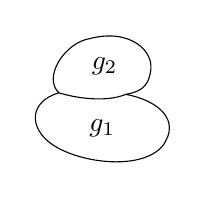
\begin{tikzpicture}
\draw (-0.55,0.42) .. controls (-0.76,0.61) and (-0.48,1.06) .. (-0.15,1.11)
  .. controls (0.35,1.24) and (0.68,0.95) .. (0.61,0.67)
  .. controls (0.58,0.49) and (0.47,0.43) .. (0.30,0.40)
  .. controls (0.03,0.29) and (-0.36,0.36) .. (-0.55,0.42);
\draw (-0.55,0.42) .. controls (-0.93,0.31) and (-0.94,-0.03) .. (-0.63,-0.24)
  .. controls (-0.27,-0.48) and (0.51,-0.57) .. (0.77,-0.25)
  .. controls (1.00,0.07) and (0.72,0.32) .. (0.30,0.40);
\node at (0,-0.03) {$g_1$};
\node at (0.03,0.76) {$g_2$};
\end{tikzpicture}
\end{adjustbox}
\end{center}

Так и будет, если добавить член (5).

[Волнистым подчёркнуто:] \underline{awkward} --- неуклюжий

Тогда

\begin{equation*}
C=-\frac{1}{8\pi G}\int K^0(\pm h)^{1/2}\,d^3x \tag{7}
\end{equation*}
\Unclear{GELFAND-P000879}{equation-07-superscript}{$K^0$ или $K^{\circ}$}

[Внизу зачёркнуто: \Unclear{GELFAND-P000879}{bottom-cancelled-fragment}{неразборчиво}.]

\SourcePage{GELFAND-P000880}{unlabelled}
\underline{\underline{Баталин.}}

\underline{Квантование систем со связями.}

\underline{2 рода связей}: 1-го и 2-го родов.

\Unclear{GELFAND-P000880}{top-short-sentence}{Эффект. не решаются.}

Надо писать гамильт. контин. интеграл со связями
\begin{equation*}
q^i,p_i\text{ — кан. координаты},\qquad M\text{ — фаз. пр-во}
\tag{1}
\end{equation*}
$i=1,\ldots,n$.

$q^i,p_i$ могут быть чётными или нечётными; есть скобка
\begin{equation*}
H_0(q,p)\text{ — гамильтониан},\quad T_\alpha(q,p)\text{ — связи},\quad
\alpha=1,\ldots,2m.
\tag{2}
\end{equation*}
\begin{equation*}
\{A,B\}=\frac{\partial_r A}{\partial q^i}\frac{\partial_\ell B}{\partial p_i}
-(-1)^{n_A n_B}\frac{\partial_r B}{\partial q^i}\frac{\partial_\ell A}{\partial p_i}
\tag{3}
\end{equation*}
[В знаменателе второй производной по $q^i$ снизу зачёркнут индекс:
\Unclear{GELFAND-P000880}{eq03-cancel-index}{$i$?}.]

$n_A,n_B$ — чётности.
\begin{equation*}
\{B,A\}=-(-1)^{n_A n_B}\{A,B\}
\tag{4}
\end{equation*}
отсюда
\begin{equation*}
\{A,A\}=-(-1)^{n_A}\{A,A\}
\tag{5}
\end{equation*}
BRS — симметрия

($\underline{\mathrm{Becchi},\ \mathrm{Rouet},\ \mathrm{Stora}}$).
\begin{equation*}
(-1)^{n_A n_C}\{\{A,B\}C\}+\text{цикл. }(A,B,C)=0
\tag{6}
\end{equation*}
\Unclear{GELFAND-P000880}{eq06-separator}{Между внутренней скобкой и $C$ запятая не видна.}

При квантовании:
\begin{equation*}
\{A,B\}\mapsto[A,B]=AB-(-1)^{n_A n_B}BA
\tag{7}
\end{equation*}
\underline{Определение}
\begin{equation*}
\left.\operatorname{Det}_{\pm}\{T_\alpha,T_\beta\}\right|_{T=0}\ne0
\quad\text{— связи 2-го рода}
\tag{8}
\end{equation*}
[Под $\operatorname{Det}_{\pm}$ вертикально приписано: $\Vert\,\mathrm{def}$; ниже — $\mathrm{Ber}$.]
\begin{equation*}
\left.
\begin{aligned}
(9)\qquad &\left.\operatorname{Det}_{\pm}\{T_\alpha,T_\beta\}\right|_{T=0}=0\\
(9)_2\qquad &\left.\{H_0,T_\alpha\}\right|_{T=0}=0
\end{aligned}
\right\}\quad\text{— связи 1-го рода}
\end{equation*}
\Unclear{GELFAND-P000880}{eq09-degeneracy}{В (9) записано обращение определителя в нуль.}

квант. связей 1-го рода свод. к связям 2-го рода (будет ниже)

\underline{Рассм. связи 2-го рода.}

Классич. динамика — нах. усл. экстремума классич. действия
\begin{equation*}
S[q,p]=\left.\int dt\,(p_i\dot q^i-H_0)\right|_{T=0}
\tag{10}
\end{equation*}
Это эквив. зад. на безусл. экстремум:

\SourcePage{GELFAND-P000881}{39}
\begin{equation*}
S[q,p,\lambda]=\int dt\,(p_i\dot q^i-H_0-T_\mu\lambda^\mu)
\tag{11}
\end{equation*}
\underline{Скобка Дирака:}
\begin{equation*}
\{A,B\}_D\underset{\mathrm{def}}{=}
\{A,B\}-\{A,T_\alpha\}(Q^{-1})^{\alpha\beta}\{T_\beta,B\}
\tag{12}
\end{equation*}
Здесь:
\begin{equation*}
Q_{\alpha\beta}=\{T_\alpha,T_\beta\}
\tag{13}
\end{equation*}
(\underline{И.М.Г.}: это скобка, постр. по сужению симп. формы на подмн-ие).

Рассм. ур-е экстремалей этого действия:
\begin{equation*}
\left\{
\begin{aligned}
\dot q^i&=\{q^i,H_0\}_D\\
\dot p_i&=\{p_i,H_0\}_D\\
\lambda^\alpha&=-(Q^{-1})^{\alpha\beta}\{T_\beta,H_0\}
\end{aligned}
\right.
\tag{14}
\end{equation*}
[После последней скобки затушёван знак:
\Unclear{GELFAND-P000881}{eq14-final-blot}{$D$?}.]

Получаются станд. ур-я Гамильтона;
но роль скобки — скобка Дирака.

Отсюда — именно её \Unclear{GELFAND-P000881}{commutator-word}{на} заменять на коммутатор.

Из [зачёркнуто: \Unclear{GELFAND-P000881}{before-eq15-cancel}{$T$?}] ур-я
\begin{equation*}
T_\alpha(q,p)=0
\tag{15}
\end{equation*}
выразим
\begin{equation*}
q^i=q^i(q^*,p^*),\quad p_i=p_i(q^*,p^*)
\tag{16}
\end{equation*}
$*=1,\ldots,n-m$

Хотим, чтобы $q^*,p_*$ были каноническими, т.е.
\begin{equation*}
\left.\int p_i\dot q^i\,dt\right|_{T=0}=\int p_*\dot q^*\,dt
\tag{17}
\end{equation*}
[У $p_*$ справа зачёркнут верхний знак:
\Unclear{GELFAND-P000881}{eq17-upper-star}{$*$?}.]

\underline{Ур-е будет иметь вид:}
\begin{equation*}
\dot q^*=\{q^*,H^{\mathrm{phys}}\}\qquad\text{и то же для }p.
\tag{18}
\end{equation*}
\begin{equation*}
H^{\mathrm{phys}}(q^*,p_*)=\left.H_0(q,p)\right|_{T=0}
\tag{19}
\end{equation*}
Это следствие обычных св-в скобки Пуассона
\begin{equation*}
\left.\{A,B\}_D\right|_{T=0}=\text{[зачёркнуто]}\quad\{A^*,B^*\},
\tag{20}
\end{equation*}
[Зачёркнутое после знака равенства:
\Unclear{GELFAND-P000881}{eq20-cancel}{$\displaystyle\sum_*\frac{\partial A^*}{\partial q^*}$?}.]

где
\begin{equation*}
A^*(q^*,p^*)=A\bigl(q(q^*,p^*),p(q^*,p^*)\bigr)
\tag{21}
\end{equation*}

\SourcePage{GELFAND-P000882}{unlabelled}
\underline{Квантование}

Без связей; пусть дан гамильтониан $H(q,p)$ и действие

[Зачёркнуто перед $S(q,p)$:
\Unclear{GELFAND-P000882}{eq22-cancel}{$H(q,p)$?}.]
\begin{equation*}
S(q,p)=\int dt\,(p\dot q-H)
\tag{22}
\end{equation*}
Ур-я:
\begin{equation*}
\dot q=\{q,H\}\qquad\text{и то же для }p
\tag{23}
\end{equation*}
\underline{Квантование}: велич. зам. операторами, и вып. ур-я
\begin{equation*}
\dot q=\frac1i[q,H],\quad\ldots
\tag{24}
\end{equation*}
и коммут. соотн.
\begin{equation*}
\frac1i[q^i,p_j]=\{q^i,p_j\}=\delta^i_j
\tag{25}
\end{equation*}
[В первой скобке под $q^i$ зачёркнут нижний индекс:
\Unclear{GELFAND-P000882}{eq25-cancel-subscript}{$i$?}.]

Рассмотрим:
\begin{equation*}
Z(J,I)=\langle0|T e^{-i\int H_{\mathrm{ext}}\,dt}|0\rangle
\tag{26}
\end{equation*}
$\langle0|$ — вектор осн. сост. в нач. момент

\hspace{3em}(произв. нач. вектор

$T$ — станд. $T$-произведение (расстан. опер. по возр. времени).

Здесь:
\begin{equation*}
H_{\mathrm{ext}}=-J_iq^i-p_iI^i
\tag{27}
\end{equation*}
[В конце (27) зачёркнуты знаки:
\Unclear{GELFAND-P000882}{eq27-cancel}{$q$?; $+H$?; $H$?}.]

(операторы здесь развив. по времени с пом. ур-й (24) —
\newline
—так входит $H$).

\underline{Ур-я по источникам.} (следуют отсюда)

[Зачёркнуто:
\Unclear{GELFAND-P000882}{before-eq28-cancel}{$\dot q=\{q,H\}$?; $\dot q-\{q,H\}$?}.]
\begin{equation*}
\left.\bigl(\dot q-:\{q,H+H_{\mathrm{ext}}\}:\bigr)\right|_{\substack{
q=\frac{\delta_r}{i\delta J}\\
p=\frac{\delta_\ell}{i\delta I}}}Z=0
\tag{28}
\end{equation*}
$:\ldots:$ — все источники став. \underline{\underline{слева}} от опер. диффер.

[Под словами «все источники»: $I$ и $J$.]

Ур-е (28) реш. с пом. преобр. Фурье:
\begin{equation*}
Z=N\int[dq][dp]\,\exp\left\{i\int dt\,(p\dot q-H-H_{\mathrm{ext}})\right\}
\tag{29}
\end{equation*}
$N$ — нормир. постоянная.

[На правом поле:] $T$-произв. недоопред. (в один мом. вр. оно не различает опер.)

\underline{Со связями 2-го рода.}

Скобка Дир. $\rightsquigarrow$ коммут.

надо зад. одноврем. коммут. соотн.

\SourcePage{GELFAND-P000883}{40}

\begin{equation*}
\frac{1}{i}[q^i,p_j]=\{q^i,p_j\}_D
=\delta^i_j-\{q^i,T_\alpha\}(Q^{-1})^{\alpha\beta}\{T_\beta,p_j\}
\tag{30}
\end{equation*}

(31) Ур-е (28) то же, но стоит в нём скобка Дирака

Решается опять методом Фурье:

Ответ:

\begin{equation*}
Z=\int[dq][dp]\exp\left\{i\int dt(p\dot q-H_0)\right\}
\prod_t\delta(T(q,p))
\bigl(\operatorname{Det}_{\pm}\{T,T\}\bigr)^{1/2},
\tag{32}
\end{equation*}
\Unclear{GELFAND-P000883}{eq32-h-index}{В (32) индекс у $H$: $0$?; густо затушёван.}

Здесь:

[Справа:] $\delta$ — $(2m)$-мерная $\delta$-ф-я.

\begin{equation*}
H=H_0+H_{ext}
\tag{33}
\end{equation*}

\underline{О связях 1-го рода.}

Пусть есть связи $T'_\alpha$, $\alpha=1,\ldots,2m$, 1-го рода

$T''$ — связи 2-го рода.

Действие

\begin{equation*}
S=\int dt(p\dot q-H)\big|_{T=0}
\tag{34}
\end{equation*}

инвариантно отн. преобразований

\begin{equation*}
\delta^Fq=[q,T'_\alpha]F^\alpha
\tag{35}
\end{equation*}

$F^\alpha=F^\alpha(t)$ — параметр!

Это и есть калибр. инвар. в гам. формализме.

Динамика не фиксир. связями однозн.

Надо из каждого кл. выбрать предст. — калибровка!

[Приписано над (36):] Добавим новые связи:
[стрелка вниз к $\Phi_\alpha=0$.]

\begin{equation*}
T'_\alpha=0,\qquad \Phi_\alpha=0
\tag{36}
\end{equation*}

так, что

\begin{equation*}
\operatorname{Det}\{\Phi,T'\}\ne0
\tag{37}
\end{equation*}

\begin{equation*}
\psi=\begin{pmatrix}T'\\\varphi\end{pmatrix}
\quad\text{— связь 2-го рода!}
\end{equation*}
\Unclear{GELFAND-P000883}{combined-constraint-symbol}{Знак слева от столбца: $\psi$ или $\Psi$; регистр неясен.}
[Слова «связь 2-го рода!» подчёркнуты волнистой чертой.]

Ответ уже написан

\begin{equation*}
Z'=\int[dq][dp]\exp\left\{i\int dt(p\dot q-H)\right\}
\prod_t\delta(T'(q,p)\operatorname{Det}\{\varphi,T'\}\delta(\varphi(q,p))
\end{equation*}
\Unclear{GELFAND-P000883}{final-delta-parenthesis}{После $T'(q,p)$ перед $\operatorname{Det}$ видна одна закрывающая скобка; скобка первого $\delta$ не закрыта.}

Независимость от $\varphi$ прослеж. с пом. BRS-симметрии.

\SourcePage{GELFAND-P000884}{unlabelled}

\underline{19.11.79.}\qquad\underline{\underline{Сем. Гельфанда.}}

\underline{Где встречаются дилогарифмы?}

\begin{enumerate}
\item[1)] $K$-теория (Bloch, Бейлинсон.)
\item[2)] комбинат. теория хар. классов (Г.-Г.-Л.)
\item[3)] объём неевклидова тетраэдра (Гаусс, ---)
\item[4)] $\zeta(3)$ (Apéry)
\item[5)] Ткани (Боль и др.)
\end{enumerate}

[Справа, на уровне пункта 1:]
6) Теория рассеяния

\Unclear{GELFAND-P000884}{dilogarithm-heading-ending}{Дилогарифм: / Дилогарифмы: [последние штрихи затушёваны]}

\begin{equation*}
\int_0^\xi\frac{\log x}{1-x}\,dx
\tag{1}
\end{equation*}

\begin{equation*}
\sum_{j=1}^{5}\left(\frac{\log u_j}{1-u_j}+\frac{\log(1-u_j)}{u_j}\right)du_j=0
\tag{2}
\end{equation*}

\SourcePage{GELFAND-P000885}{unlabelled}
\underline{Бейлинсон}

\begin{equation}
\int_0^1\frac{\ln x}{1-x}\,dx=\sum\frac{1}{n^2}
\tag{3}
\end{equation}
\Unclear{GELFAND-P000885}{equation-03-sign}{В (3) минус перед суммой не написан; знак сохранён по источнику.}

Обобщение на случай кривых

(Bloch)

Справа $\zeta(2)\rightsquigarrow\zeta$ замен. на $\zeta$-ф-ю кривой.

$X$ — рим. поверхность над $\mathbb C$ (не обяз. компактная)

$f,g$ — обратимые голом. ф-и на $X$. Рассм. форму:
\begin{equation}
\omega_{f,g}=\ln|f|\,d(\arg g)-\ln|g|\,d(\arg f)
\tag{4}
\end{equation}

Св-ва:
\begin{equation}
\text{1) }d\omega_{f,g}=0\Rightarrow\text{кор. опр. интегр. по любым путям}
\tag{5}
\end{equation}
\begin{equation}
\text{2) }\omega_{f_1f_2,g}=\omega_{f_1,g}+\omega_{f_2,g}
\tag{6}
\end{equation}
\begin{equation}
\text{3) }\omega_{f,g}+\omega_{g,f}=0
\tag{7}
\end{equation}
\begin{equation}
\text{4) }\omega_{f,1-f}\quad\text{точна, если }f\text{ и }1-f\text{ не обр. в }0
\tag{8}
\end{equation}
(тожд. Стейнберга)

\begin{equation*}
X=\mathbb C P^1\setminus\{0,1,\infty\}
\end{equation*}
$f=t$ — станд. параметр.

Тогда

\Unclear{GELFAND-P000885}{cancelled-omega}{Зачёркнутая строка: $\omega_{t,1-t}=\ln|t|\arg(1-t)$; последние знаки неразборчивы.}

\begin{equation}
\int_0^\xi\omega_{t,1-t}=\ln|\xi|\arg(1-\xi)-\operatorname{Im}\int_0^\xi\ln(1-t)\,d(\ln t)
\tag{9}
\end{equation}
Справа стоит однозначная ф-я!! — можно показать

D. Wigner придумал и связал с непр. когомологиями $SL(2)$.

(сын)

5) Рассм. цикл
\SourceFigure{GELFAND-P000885}{cycle-loop}{Маленькая петля с внутренней отметкой, похожей на $x$. Направление обхода неразборчиво. Подобный знак повторён под интегралом в (10).}
обх. одну из выкол. точек $x$. Тогда
\begin{equation}
\int_{\text{[тот же цикл]}}\omega_{f,g}=\ln\left|\frac{f^{v_x(g)}}{g^{v_x(f)}}\right|(x),
\tag{10}
\end{equation}
\Unclear{GELFAND-P000885}{equation-10-normalization}{В (10) перед логарифмом нет множителя; нормировка интеграла по циклу не пояснена.}

$v_x(g)$ — порядок нуля $g$ в точке $x$.

(алгебр. кривая однозначно компактифицируется — напр., вложим
в проект. пр-во и замкнём)

Отсюда получается отображение
\begin{equation}
K_2(X)\to H^1(X,R)
\tag{11}
\end{equation}
$f,g$ — ф-и на $X$, не обр. в $0$ ни в какой точке.

Рассм. $\{f,g\}$ — своб. группу и факторизуем по соотношениям 2), 3), 4),

[«2)» вписано над строкой с указателем перед «3)».]

\SourcePage{GELFAND-P000886}{47}
с соотн. бимультипл. и т. д.

$\omega_{f,1-f}=0$ в $H^1(X,R)$, т. е. $\{f,1-f\}=0$.

Это $K_2(X)$ от поля рац. ф-й на кривой.

$K_2(X)$ Опред. с пом. точной последовательности:
\begin{equation}
\begin{aligned}
K_2(X)&\to K_2(\mathbb C(X))\to\bigoplus_{x\in X}\mathbb C^*\\
&\{f,g\}\longrightarrow\sum_{x\in X}(-1)^{v_x(f)v_x(g)}\frac{f^{v_x(g)}}{g^{v_x(f)}}
\end{aligned}
\tag{12}
\end{equation}

Из тождества (10) вытекает, что есть \underline{единственное корректное
отображение} (11). Рассм. лин. комбинацию

\Unclear{GELFAND-P000886}{cancelled-before-13}{Перед суммой в (13) зачёркнут одиночный знак; неразборчиво.}
\begin{equation}
\sum n_i\{f_i,g_i\}\in K_2(\mathbb C(X))
\tag{13}
\end{equation}
Выбросим нули и полюса, интегралы по петлям $=0$

$\Rightarrow$ получ. класс когомологий из $H^1(X,R)$ после взятия диффер.
\begin{equation}
\left\{\sum n_i\omega_{f_i,g_i}\right\}.
\tag{14}
\end{equation}

Есть конструкция

\SourceFigure{GELFAND-P000886}{diagram-15}{(15) Треугольная схема. Слева вверху $K_2(X)$, справа вверху $H^1(X,R)$, справа внизу $H^1(X,\mathbb C^*\text{ [зачёркнуто]})$. Верхняя горизонтальная стрелка направлена от $K_2(X)$ вправо; диагональная — от $K_2(X)$ к нижнему правому узлу; правая вертикальная — снизу вверх, с подписью $\ln|\ |$. Зачёркнутые знаки после $\mathbb C^*$ неразборчивы.}

Определим
\begin{equation}
\int_\gamma\{f,g\}=\begin{cases}
(-1)^{v_\gamma(f)v_\gamma(g)}\exp\frac{1}{2\pi i}\int_\gamma\left(\ln f-\frac{v_\gamma(f)}{v_\gamma(g)}\ln g\right)d\ln g,&v_\gamma(g)\ne0\\
\exp\frac{1}{2\pi i}\int-\ln g\,d(\ln f)
\end{cases}
\tag{16}
\end{equation}
(Бейлинсон)

Этот символ бимульт., симм., уд. тожд. Стейнберга и
после интегр. даёт предыдущий.
\Unclear{GELFAND-P000886}{symbol-symmetry}{Написано «симм.»; возможное математическое несоответствие оставлено без исправления.}

$X$ — афф. кривая $\Rightarrow$
\begin{equation}
K_2(X)=H_2(SL_n(\text{алг. ф-и на }X),\mathbb Z)
\tag{17}
\end{equation}
\begin{equation}
1\to K_2(X)\to St^X\to SL^X\to1
\tag{18}
\end{equation}
(см. Милнор и Стейнберг).

— $\cdot$ —

\SourcePage{GELFAND-P000887}{unlabelled}
\underline{\underline{Баталин.}}

О квантовании систем со связями в релятивистской калибровке.

[Под заголовком — волнистая линия.]

\begin{equation}
S=\int(p\dot q-H_0-\lambda T)\,dt
\tag{1}
\end{equation}
\begin{equation}
\varphi=\begin{pmatrix}q\\\lambda\end{pmatrix}\quad\text{— релятив. поле;}
\tag{2}
\end{equation}
В электродин.
\begin{equation}
\begin{pmatrix}\vec A\\A\end{pmatrix}
\tag{3}
\end{equation}
\Unclear{GELFAND-P000887}{cancelled-after-03}{Справа вверху от скобки в (3) зачёркнут небольшой знак; неразборчиво.}
— где $A$ — $\lambda$-множитель связи.

В гравитации $\varphi^\alpha(q,p)$, $g^{0\alpha}$.

Теперь
\begin{equation}
S=\int\left(p\dot q-H_0-\lambda_\mu T^\mu\ \text{[неясный знак]}\ \tilde\pi_\mu\varphi^\mu\right)
\tag{4}
\end{equation}
\Unclear{GELFAND-P000887}{equation-04-overwritten-sign}{Знак перед $\tilde\pi_\mu\varphi^\mu$ густо перезаписан; возможны минус или плюс, надёжно не читается.}

[Пометы с указателями к (4): над $\varphi^\mu$ — «калибр. ф-и»;
под $T^\mu$ — «связи 1-го рода»;
под $\tilde\pi_\mu$ — «лагр. мн. калибр.».]

\begin{equation*}
\Phi=\Phi(p,q)
\end{equation*}
Релятив. инвар. калибр. условие
\begin{equation}
\Phi^\mu(p,q,\lambda,\dot\lambda)=-\dot\lambda^\mu+\chi^\mu(\lambda,p,q,\tilde\pi)
\tag{5}
\end{equation}
\Unclear{GELFAND-P000887}{equation-05-first-argument}{Первый аргумент $\chi^\mu$ густо перезаписан; чтение $\lambda$ вероятно, но не вполне надёжно.}

\begin{equation}
\left\{
\begin{aligned}
q^A&=\begin{pmatrix}q^i\\\lambda^\mu\end{pmatrix},\quad p_A=(p_i,\bar\pi_\mu),\quad A=1,\ldots,n+m;\\
G_a&=(\bar\pi_\mu,T_\mu),\quad a=1,\ldots,2m;\quad\chi^a=-\begin{pmatrix}\chi^\mu\\\lambda^\mu\end{pmatrix}
\end{aligned}
\right.
\tag{6}
\end{equation}
\Unclear{GELFAND-P000887}{pi-overstroke}{Над $\pi$ в (4), (5) штрих волнистый, в (6) почти прямой. Передано соответственно $\tilde\pi$ и $\bar\pi$; различие обозначений не установлено.}

\Unclear{GELFAND-P000887}{cancelled-before-relative}{Перед «Это релятив. фаз. пр-во.» зачёркнут одиночный знак; неразборчиво.}
Это релятив. фаз. пр-во. Тогда
\begin{equation}
\begin{aligned}
S=S'[q^A,p_A]&=\int dt(p_A\dot q^A-H_{n+m});\\
H_{n+m}&=H_0-G_a\chi^a.
\end{aligned}
\tag{7}
\end{equation}
\Unclear{GELFAND-P000887}{equation-07-prime}{Над правым краем второго $S$ есть короткий штрих: возможно $S'$, возможно конечный штрих самой буквы $S$.}
Здесь явно выражено, что возросло число переменных

(а на самом деле $(n-m)$)

\begin{equation*}
n-m=(n+m)-2m
\end{equation*}
Надо подавить $2m$ лишних степ. свободы.
\begin{equation}
Z=\int\left(\prod_{t,A,a}dq^A\,dp_A\,d\eta^a\,d\mathcal P_a\right)\exp\left\{i\int dt\left(p_A\dot q^A+\mathcal P_a\dot\eta^a-H_{\mathrm{complete}}\right)\right\}
\tag{8}
\end{equation}
где
\begin{equation}
H_{\mathrm{complete}}=H_1-\{\Psi,\Omega\}.
\tag{9}
\end{equation}
\SourcePage{GELFAND-P000888}{48}
Здесь $H_1$ и $\Omega$ нах. из ур-й:
\begin{equation}
\{\Omega,\Omega\}=0,\qquad \{H_1,\Omega\}=0
\tag{10}
\end{equation}
\begin{equation}
\Psi=\mathcal P_a\chi^a
\tag{11}
\end{equation}
$\Psi,\Omega$ — фермионные перем.

Если связи 1-го рода, то ур-я решаются в виде рядов по степ.
$\eta^a$ и $\mathcal P_a$; в супергравит. имеют обыкн. обрываться.

Суперграв. — инв. отн.
[Зачёркнуто: \Unclear{GELFAND-P000888}{middle-cancelled}{неразборчиво}.]
BRS-преобр.:
\begin{equation}
\delta X=\{X,\Omega\}\mu,\qquad
\mu\text{ — нечётная перем. (постоянная).}
\tag{12}
\end{equation}
$\Omega$ — фермион

выберем:
\begin{equation}
\mu=i\int dt\,\mathcal P_a\,\delta\chi^a
\tag{13}
\end{equation}
Получается BRS-инвар.

\underline{Один понедельник пропускается.}
[Волнистое подчёркивание.]

\SourcePage{GELFAND-P000889}{unlabelled}
\underline{\underline{3.12.79.}}
\qquad \underline{Сем. Гельфанда}

\underline{\underline{Физик}}.
\quad \underline{О соврем. теории элем. частиц.}

\begin{equation*}
\mathrm{QCD}\text{ — сильное}\qquad
1972\text{ (оконч. ред.)}\qquad\text{Gell-Mann}
\end{equation*}
\begin{equation*}
\underbrace{\mathrm{QED}+\text{слабое}}_{\text{кв. эл.-дин.}}
\Longrightarrow\mathrm{QFD}
\qquad
\begin{gathered}
1967\text{ (Вайнберг, Салам)}\\
\text{Глэшоу}
\end{gathered}
\end{equation*}
[«Глэшоу» вписано ниже фамилий.]

$\mathrm{GR}$\qquad Экспер. факты — лагранжианы правильные

\underline{Фаддеев, Славнов} — вычисления
\Unclear{GELFAND-P000889}{middle-computations}{непротив-чивые}
[Фамилии подчёркнуты волнистой линией.]

\underline{Нужно:}

1) предст. групп

2) диагр. Фейнмана (см. Бьёркен, Дрелл, т. 1)

Путь от лагранжианов к эксп. данным — короткий !!

\begin{center}
\begin{adjustbox}{max width=\linewidth}
\begin{tikzpicture}[x=1cm,y=1cm]
\node at (0,0) {$P$};
\node at (1.2,0) {$N$};
\node at (2.3,0) {$e$};
\node at (3.25,0) {$\nu$};
\draw (0,-0.20) -- (0,-0.65);
\draw (1.2,-0.25) -- (1.35,-0.70);
\draw (2.55,-0.36) .. controls (2.9,-0.43) and (3.1,-0.63) .. (3.15,-0.82);
\draw (3.6,-0.12) -- (5.6,-0.42);
\node at (0.05,-1.1) {протон};
\node at (1.8,-1.1) {нейтрон};
\node at (4,-1.1) {электрон};
\node at (6,-1.05) {нейтрино};
\end{tikzpicture}
\end{adjustbox}
\end{center}

[Ниже слова «протон» зачёркнут знак:
\Unclear{GELFAND-P000889}{lower-left-cancelled}{$P$?}.]

\begin{center}
\begin{adjustbox}{max width=\linewidth}
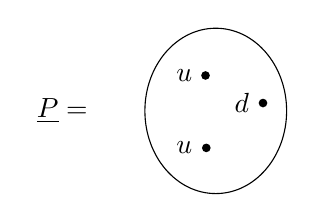
\begin{tikzpicture}[x=1cm,y=1cm]
\node at (-1.9,0) {$\underline{P}={}$};
\draw (0,0) ellipse (0.9 and 1.05);
\node at (-0.4,0.45) {$u$};
\fill (-0.13,0.45) circle (0.055);
\node at (0.33,0.10) {$d$};
\fill (0.60,0.10) circle (0.055);
\node at (-0.4,-0.47) {$u$};
\fill (-0.12,-0.47) circle (0.055);
\end{tikzpicture}
\end{adjustbox}
\qquad
$\begin{gathered}
\underset{\text{заряды}}{\begin{pmatrix}0\\-1\end{pmatrix}}
\quad\begin{pmatrix}\nu\\e\end{pmatrix}\text{ — спинор (!)}\\[1.2em]
\underbrace{\begin{pmatrix}u\\d\end{pmatrix}}_{\substack{\text{тоже}\\\text{что-то вроде спинора}}}
\quad
\underset{\text{\fbox{заряды}}}{\begin{pmatrix}\tfrac23\\-\tfrac13\end{pmatrix}}
\end{gathered}$
\end{center}

\SourcePage{GELFAND-P000890}{unlabelled}
Нельзя избегать дробей (сделать заряды ед. матрицей)

\begin{equation*}
\begin{pmatrix}\nu\\e\end{pmatrix}
\qquad
\begin{pmatrix}u\\d\end{pmatrix}
\text{ — основные элем. частицы.}
\end{equation*}
[Справа:] \underline{(I-е поколение)}\quad\underline{частиц}

Они достаточны для постр. окруж. мира

\begin{center}
\begin{adjustbox}{max width=\linewidth}
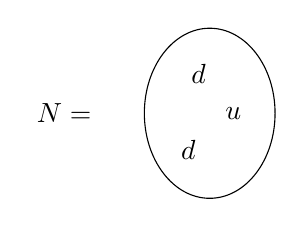
\begin{tikzpicture}[x=1cm,y=1cm]
\node at (-1.8,0) {$N={}$};
\draw (0,0) ellipse (0.83 and 1.08);
\node at (-0.14,0.50) {$d$};
\node at (0.30,0.0) {$u$};
\node at (-0.27,-0.47) {$d$};
\end{tikzpicture}
\end{adjustbox}
\end{center}

Есть другие поколения

\begin{center}
\begin{adjustbox}{max width=\linewidth}
\begin{tikzpicture}[x=1cm,y=1cm]
\node at (0,0) {$\begin{pmatrix}\nu_e\\e\end{pmatrix}$};
\node at (2.9,0) {$\begin{pmatrix}\nu_\mu\\\mu\end{pmatrix}$};
\node at (5.8,0) {$\begin{pmatrix}\nu_\tau\\\tau\end{pmatrix}$};
\node[anchor=west] at (0.32,-0.43) {$\underline{0,5}\,\text{МэВ}$};
\node[anchor=west] at (3.22,-0.43) {$100\,\text{МэВ}$};
\node[anchor=west] at (6.12,-0.43) {$1800\,\text{МэВ}$};
\node[anchor=west] at (7.75,0.96) {не давно};
\draw[->] (7.62,0.83) -- (6.46,0.32);
\draw[->] (9.10,-0.43) -- (8.36,-0.43);
\node[anchor=west] at (9.2,-0.43) {массы};
\node at (11.25,0.0) {$\mathrm{QFD}$};
\node at (0,-1.85) {$\begin{pmatrix}u\\d\end{pmatrix}$};
\node at (2.9,-1.85) {$\begin{pmatrix}c\\s\end{pmatrix}$};
\node at (5.8,-1.85) {$\begin{pmatrix}t\\b\end{pmatrix}$};
\draw[->] (6.92,-1.51) -- (6.29,-1.51);
\node[anchor=west] at (7.05,-1.51) {пока не найден};
\node at (11.25,-1.85) {$\mathrm{QCD}$};
\draw[->] (0,-3.37) -- (0,-2.50);
\node at (0,-3.72) {\underline{I поколение}};
\end{tikzpicture}
\end{adjustbox}
\end{center}

Верхние — \underline{\Unclear{GELFAND-P000890}{leptons-overwrite}{лептоны}} (лёгкие)
[В окончании подчёркнутого слова наложены штрихи.]

\begin{equation*}
m_p\sim940\,\mathrm{MeV}
\end{equation*}

След. поколения появляются, быстро исчезают.

Лептоны уч. лишь в дин. ароматов — эл.-магн. и слабые-взаим

(flavour dinamics)

Каждый кварк утроен:
\begin{equation*}
\begin{gathered}
u^1,u^2,u^3\\
d^1,d^2,d^3
\end{gathered}
\qquad
\begin{gathered}
\text{и так со }\underline{\text{всеми кварками}}\\
(c,s,t,b)
\end{gathered}
\end{equation*}

Соотв. симметрия:

каждый кварк — представлени\Unclear{GELFAND-P000890}{representation-overwrite}{е} $SU(3)$
[Окончание слова переписано поверх прежних штрихов.]

\begin{equation*}
\fbox{$u^1,u^2,u^3\qquad SU(3)_c$}
\qquad C\text{ — от }\underline{\text{colour}}\text{ (цвет)}
\end{equation*}
[Под $SU(3)_c$ короткая линия к подписи:]

группа \Unclear{GELFAND-P000890}{lower-group-word}{неразборчиво} по сопр. предст.

Нарисуем поколения на 3-мерной диаграмме

\SourceFigure{GELFAND-P000890}{diagram-generations}{Внизу слева пространственная схема. Из общей закрашенной точки с подписью $u^1$ идут линия вверх, почти горизонтальная линия вправо и линия наклонно вниз влево. На вертикальной линии выше $u^1$ отмечены закрашенные точки $u^2$ и $u^3$; линия продолжается выше $u^3$. На наклонной линии ниже и левее $u^1$ находятся закрашенная точка $d^1$, затем незакрашенные кружки $\nu$ и $e$. От $d^1$ вверх идёт тонкая прерывистая линия с закрашенными точками $d^2$ и $d^3$. На горизонтальной линии правее $u^1$ имеется закрашенная точка с неясной подписью, похожей на $c$, $t$ или $\tau$, и малым верхним штрихом. От этой точки продолжается тонкая вертикальная линия вверх; вниз влево виден короткий наклонный отрезок. Ниже расположена вторая наклонная линия с закрашенной точкой $s$ и незакрашенными кружками $\nu_\mu$ и $\mu$. От $s$ вверх идёт ещё одна тонкая прерывистая вертикальная линия, пересекающая горизонталь между $u^1$ и неясно подписанной точкой. Наклонные отрезки у верхней неясно подписанной точки и у $s$ не соединены уверенно читаемым непрерывным штрихом. Под правой частью горизонтали написано «след. покол.». Надёжно различимых наконечников стрелок нет.}

[Справа от схемы:]

$SU(3)_c$ меняет вертик. сост.

(все вертик. сразу обслуживает)

лептоны не утроены

(только кварки)

\SourcePage{GELFAND-P000891}{59}
Действие группы.
\begin{equation*}
\lvert d^{1'}\rangle=U_{11}\lvert d^1\rangle+U_{12}\lvert d^2\rangle+U_{13}\lvert d^3\rangle
\end{equation*}
$U$ — унит. матрица.

Или.
\begin{equation*}
\lvert d^{1'}\rangle=U^1_1\lvert d^1\rangle+U^1_2\lvert d^2\rangle+U^1_3\lvert d^3\rangle
\end{equation*}

Лептоны переставл. тоже!! — приближенно (массы разные)

\Unclear{GELFAND-P000891}{weak-group-word}{Группа / Группы}
перест. $SU(2)_w$ (Вайнберговская группа)

\SourceFigure{GELFAND-P000891}{weak-doublets}{Четыре обведённые овалами вертикальные пары, расположенные в два ряда: сверху слева $u_1$ над $d^1$, сверху справа $c$ над $s$; снизу слева $\nu$ над $e$, снизу справа $\nu_\mu$ над $\mu$. Справа от овалов две стрелки направлены влево, одна вверх, другая вниз, к двум рядам пар. Положение индекса 1 у $u$ требует сверки; у $d$ индекс 1 написан вверху.}

синхронно в каждой паре перест. част.
с \Unclear{GELFAND-P000891}{weak-group-abbreviation}{мат. / лок.} гр. $SU(2)$

Еще нужны $U(1)$
\begin{equation*}
[SU(2)\times U(1)]_w
\end{equation*}
[Зачёркнуто: \Unclear{GELFAND-P000891}{weak-phase-cancellation}{неразборчиво}.]
($U(1)$ подкруч. фазы)

Вероятно $e$ должна была бы иметь массу $0$.
При охлаждении Вселенной произошел переход.

\underline{Фермионы} (все вышеупом.) опис. ур-ем Дирака
\begin{equation*}
(i\hat\partial-m)\Psi=0 \tag{1}
\end{equation*}
\begin{equation*}
\Psi=\begin{pmatrix}\psi^1\\\psi^2\\\psi^3\\\psi^4\end{pmatrix},
\qquad i=0,1,2,3
\end{equation*}
\begin{equation*}
\hat\partial=\partial^i\gamma_i=\partial_i\gamma^i, \tag{2}
\end{equation*}
[После второго знака равенства зачёркнуто:
\Unclear{GELFAND-P000891}{dirac-cancellation}{$\gamma_i\partial^i$?}.]

где $\gamma^i$ — матрицы Дирака,
\begin{equation*}
\gamma^i\gamma^k+\gamma^k\gamma^i=2g^{ik} \tag{3}
\end{equation*}
\begin{equation*}
g^{ik}=\operatorname{diag}(1,-1,-1,-1). \tag{4}
\end{equation*}
Ур-е (1) — Лоренц-инвариантно
\begin{equation*}
\partial_t=\partial_0,\quad \partial_x=\partial_1,\quad
\partial_y=\partial_2,\quad \partial_z=\partial_3.
\end{equation*}

Вырождение дирак. частицы:
\begin{equation*}
\gamma^5=\alpha\gamma^0\gamma^1\gamma^2\gamma^3 \tag{5}
\end{equation*}
Рассм. безмассовое ур-е (1): $m=0$

$\alpha$ выберем так, чтобы в представлении
\begin{equation*}
\gamma^0=\begin{pmatrix}I&0\\0&-I\end{pmatrix},\qquad
\gamma^\alpha=\begin{pmatrix}0&\sigma^\alpha\\-\sigma^\alpha&0\end{pmatrix} \tag{6}
\end{equation*}
$\sigma^\alpha$ — матр. Паули
($\frac12\sigma^\alpha$ — генер. группы $SU(2)$)

получилось, что
\begin{equation*}
\gamma^5=-\begin{pmatrix}0&I\\I&0\end{pmatrix} \tag{7}
\end{equation*}

\begin{adjustbox}{max width=\linewidth}
\begin{tikzpicture}[x=1cm,y=1cm]
\draw[->] (0,0.2)--(0.1,1.2);
\draw (0.13,0.2)--(0.23,1.13);
\draw[->] (0.48,0.43) .. controls (0.51,-0.13) and (0.04,-0.25) .. (-0.3,0.05);
\draw[->] (0.85,1.24)--(0.3,1.24);
\node[anchor=west] at (0.9,1.24) {$p$ импульс};
\node[anchor=west] at (0.9,0.56) {— спин};
\end{tikzpicture}
\end{adjustbox}

нейтрино — лев. винт\qquad антинейтрино — прав. винт

\SourcePage{GELFAND-P000892}{unlabelled}
\begin{equation*}
\Psi_\nu=
\underset{\text{лев. винт.}}{\frac{1+\gamma^5}{2}\Psi_\nu}
+\underset{\text{пр. винт.}}{\frac{1-\gamma^5}{2}\Psi_\nu}
\end{equation*}
$\dfrac{1\pm\gamma^5}{2}$ — проекторы на инвар. подпр-ва

для нейтрино только $\dfrac{1+\gamma^5}{2}\Psi_\nu$ встр.

для электрона оба

\begin{equation*}
\begin{array}{c@{\qquad}c}
\fbox{$\begin{gathered}\dfrac{1+\gamma^5}{2}\Psi_e\\
\text{лев. эл-н}\\[6pt]
\dfrac{1+\gamma^5}{2}\Psi_\nu\end{gathered}$}
&
\fbox{$\begin{gathered}\dfrac{1-\gamma^5}{2}\Psi_e\\
\text{прав. эл-н.}\end{gathered}$}
\end{array}
\end{equation*}
[Под левой рамкой:] дублет по группе
\Unclear{GELFAND-P000892}{doublet-group}{$SU(2)\times SU(1)$}

[Под правой рамкой:] синглет по гр.
\Unclear{GELFAND-P000892}{singlet-group}{$SU(2)\times SU(1)$ / $SU(2)<SU(1)$}

[Зачёркнута формула:
\Unclear{GELFAND-P000892}{cancelled-current}{$\bar e\gamma^0(1+\gamma^5)\nu_e$?}.]

\underline{QFD}: $\underline{\gamma,\ Z^0,\ W^+,\ W^-}$

$Z^0,W^+,W^-$ — массивные.

$\gamma$ — свет

\underline{QCD}: $SU_c(3)$\qquad $8$ \underline{глюонов}

присоед. предст. в алгебре Ли

\underline{Лагранжиан.}

Сначала для вект. полей $V$

\begin{adjustbox}{max width=\linewidth}
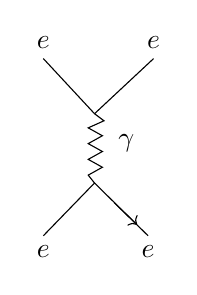
\begin{tikzpicture}[x=1cm,y=1cm]
\draw (-0.65,1.7)--(0,1);
\draw (0,1)--(0.75,1.7);
\draw (0,1)--(0.12,0.91)--(-0.08,0.82)--(0.1,0.72)--(-0.08,0.62)--(0.1,0.52)--(-0.08,0.42)--(0.1,0.32)--(-0.08,0.22)--(0,0.12);
\draw (0,0.12)--(-0.65,-0.55);
\draw (0,0.12)--(0.68,-0.55);
\draw[->] (0.25,-0.13)--(0.54,-0.41);
\node[anchor=south] at (-0.65,1.7) {$e$};
\node[anchor=south] at (0.75,1.7) {$e$};
\node[anchor=north] at (-0.65,-0.55) {$e$};
\node[anchor=north] at (0.68,-0.55) {$e$};
\node[anchor=west] at (0.18,0.63) {$\gamma$};
\end{tikzpicture}
\end{adjustbox}

\underline{фейнман. график}

$\gamma$ — кв. [Зачёркнуто:
\Unclear{GELFAND-P000892}{momentum-cancellation}{несущ.?}.]
перен. импульс

\SourceFigure{GELFAND-P000892}{charged-current-diagram}{Две вершины одна над другой соединены волнистой линией с подписью $W^-$ и направленной вверх стрелкой. От каждой вершины отходят две косые внешние линии. Верхняя левая подпись похожа на $\nu_e$ с дополнительным штрихом над или слева от $\nu$; верхняя правая подпись $e$, на этой линии стрелка идёт от вершины вверх вправо. Нижние подписи: слева $\mu^-$, справа $\nu_\mu$. Штрихи у верхней левой подписи и на верхней левой линии требуют сверки.}

перенос заряда

\begin{adjustbox}{max width=\linewidth}
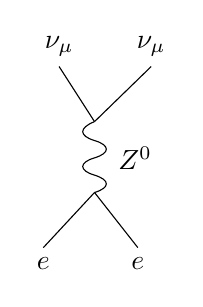
\begin{tikzpicture}[x=1cm,y=1cm]
\draw (-0.45,1.7)--(0,1);
\draw (0,1)--(0.72,1.7);
\draw (0,1) .. controls (-0.2,0.92) and (-0.2,0.82) .. (0,0.76)
.. controls (0.2,0.70) and (0.2,0.6) .. (0,0.54)
.. controls (-0.2,0.48) and (-0.2,0.38) .. (0,0.32)
.. controls (0.2,0.26) and (0.2,0.16) .. (0,0.1);
\draw (0,0.1)--(-0.65,-0.6);
\draw (0,0.1)--(0.55,-0.6);
\node[anchor=south] at (-0.45,1.7) {$\nu_\mu$};
\node[anchor=south] at (0.72,1.7) {$\nu_\mu$};
\node[anchor=north] at (-0.65,-0.6) {$e$};
\node[anchor=north] at (0.55,-0.6) {$e$};
\node[anchor=west] at (0.18,0.54) {$Z^0$};
\end{tikzpicture}
\end{adjustbox}

\begin{equation*}
\begin{array}{cccc}
83m_p&&95m_p&\\
W^+&W^-&Z^0&\gamma
\end{array}
\end{equation*}
[Две наклонные линии от области $W^+$ и от $Z^0$ к подписи:]
еще не открыты из-за большой массы
(будут в близ. пятилетке)

Заряд — соб. знач.

пары $\begin{pmatrix}e\\\nu\end{pmatrix}$ — соб. вектора

\SourcePage{GELFAND-P000893}{60}
\begin{equation*}
A_a^i,\qquad a\text{ — номер поля в присоед. предст.} \tag{8}
\end{equation*}
\begin{equation*}
F_a^{ik}=\partial^iA_a^k-\partial^kA_a^i-gf_{abc}A_b^iA_c^k \tag{9}
\end{equation*}
\begin{equation*}
\operatorname{Sp}(I_aI_b)=\frac12\delta_{ab} \tag{10}
\end{equation*}
$I_a$ — \Unclear{GELFAND-P000893}{generator-abbreviation}{опр. / опер.}
в присоед. предст. $G$
(базис)

Лагранжиан:
\begin{equation*}
-\frac14 F_a^{ik}F_a^{ik}+\bar\Psi(i\hat D)\Psi \tag{11}
\end{equation*}
\Unclear{GELFAND-P000893}{first-lagrangian-indices}{Индексы в (11).}

Здесь
\begin{equation*}
D_i=\partial_i+igI^aA_i^a \tag{12}
\end{equation*}
\begin{equation*}
\hat D=\gamma^iD_i \tag*{$(12)_2$}
\end{equation*}
[Справа зачёркнуто:
\Unclear{GELFAND-P000893}{covariant-cancellation}{$\hat D=\gamma$?}.]

Поле (11) — безмассовое

Надо ввести еще скал. поля $\Phi$ (Хиггсовские), преобр. по мультиплету

Надо:
\begin{equation*}
-\frac14F_a^{ik}F_a^{ik}+\bar\Psi(i\hat D)\Psi
+\frac12(D\varphi)^2-P(\varphi) \tag{13}
\end{equation*}
\Unclear{GELFAND-P000893}{second-lagrangian-indices}{Индексы в (13).}

Требуется
\begin{equation*}
P(\varphi)=P(g\varphi) \tag{14}
\end{equation*}
\underline{Пример}: $G=U(1)$
[Перед $P(\varphi)$ в (15): \Unclear{GELFAND-P000893}{potential-prefix-mark}{короткий толстый наклонный штрих}.]
\begin{equation*}
P(\varphi)=\lambda^2(\varphi_1^2+\varphi_2^2-\eta^2)^2 \tag{15}
\end{equation*}
($2$-я степень — $\max$ совмест. с перенормируемостью)

\underline{Классич. вакуум}: решения ур-й с $\min$ энергией, т.е.
дающие $\underline{\min P(\varphi)}$

\SourcePage{GELFAND-P000894}{unlabelled}
\underline{\underline{10.12.79.}} \qquad \underline{Сем. Гельфанда}

\underline{Тот же физик.} Было 2 лагранжиана

(\underline{Игорь Юрьевич \Unclear{GELFAND-P000894}{speaker-surname}{Кобзар-}} (?)).

\begin{equation*}
\mathcal{L}_{QCD}=-\frac14 F_a^{ik}F_a^{ik},\qquad SU_c(3)
\tag{1}
\end{equation*}
$\mathcal{L}_{FD}$ аналогично с $SU(2)\times$
[зачёркнуто: \Unclear{GELFAND-P000894}{eq1-cancelled-letter}{неразборчиво}] $U(1)$.

\begin{equation*}
F_a^{ik}\Unclear{GELFAND-P000894}{eq2-equality}{=}
\partial^i A_a^k-\partial^k A_a^i-f_{abc}A^{\Unclear{GELFAND-P000894}{eq2-overwritten-index}{b}}A^c
\tag{2}
\end{equation*}
[Под последним членом отдельно написано:]
\begin{equation*}
A^a
\end{equation*}
Отсюда легко вычисляется
\begin{equation*}
\int E^2\,dV\sim\frac{e^2}{\Unclear{GELFAND-P000894}{eq3-denominator}{r}}
\tag{3}
\end{equation*}
\SourceFigure{GELFAND-P000894}{field-lines}{Справа от (3) два небольших кружка, левый немного ниже правого; между ними почти горизонтальная линия. Над ней три выпуклые вверх дуги, под ней три выпуклые вниз дуги. Верхние дуги справа заканчиваются около правого кружка, не все явно доходят до него. Около левого конца внутренней нижней дуги утолщённый треугольный штрих, похожий на наконечник стрелки вправо; его значение неясно. Подписей не видно.}

Нелинейная среда $\Rightarrow$ силовые линии слипаются:

\SourceFigure{GELFAND-P000894}{qcd-tube}{Вытянутая горизонтальная трубка, образованная двумя дугами, с маленьким кружком на левом конце; правый конец разомкнут. Внутри ряд почти вертикальных штрихов. Слева снизу подпись QCD. Над трубкой горизонтальная скобообразная линия с опущенными вниз концами. От середины этой линии к верхнему краю трубки направлена вертикальная двусторонняя стрелка, справа от неё знак, похожий на $\ell$ или $e$. Ниже, между верхним и нижним краями трубки, ещё одна вертикальная двусторонняя стрелка с подписью $\sigma$.}

[Справа от рисунка:] \underline{Гипотеза}: сечение (или диаметр) трубки не зависит от расстояния

т.к. плотность энергии постоянна $\Rightarrow$ получ. струна
\begin{equation*}
u^1,u^2,u^3
\end{equation*}
\begin{equation*}
\Unclear{GELFAND-P000894}{tension-symbol}{\nu}=\frac{d\varepsilon}{d\ell}\sim E^2\sigma
\end{equation*}

\underline{Замеч. Манина:} при квантовании Я.-М. в квазиклассич. приближении.

(и пока нет точной модели)

\underline{Слабый лагранжиан:}
\begin{equation*}
\begin{aligned}
\mathcal{L}_{FD}&=-\frac14F_a^{ik}F_a^{ik}+\sum_{\mathrm{rep}}\bar\Psi(i\hat D)\Psi+{}\\
&\quad+\frac12(D\varphi)^2-P(\varphi);\quad\big|\,(SU(2)\times U(1))_{w,s}
\end{aligned}
\tag{4}
\end{equation*}
[Над минусом перед $P(\varphi)$ зачёркнут небольшой знак:
\Unclear{GELFAND-P000894}{eq4-cancelled-mark}{неразборчиво}.]

Здесь
\begin{equation*}
D_i=\partial_i+ig t^\alpha W_i^\alpha+ig'yB
\tag{5}
\end{equation*}
[Справа вверху при $B$ зачёркнут индекс:
\Unclear{GELFAND-P000894}{eq5-cancelled-index}{неразборчиво}.]

$t^1,t^2,t^3$ — генераторы предст. $SU(2)$

\SourcePage{GELFAND-P000895}{66}
\begin{equation*}
-\frac14F_\alpha^{ik}F_\alpha^{ik}-\frac14H^{ik}H^{ik}
+\sum_{\mathrm{rep}}\bar\Psi(i\hat D)\Psi+\frac12(D\varphi)^2-P(\varphi)
\tag{6}
\end{equation*}
[Под первым членом:] $\alpha=1,2,3.$

\begin{equation*}
F_\alpha^{ik}=\partial^iA_\alpha^k-\partial^kA_\alpha^i
-\Unclear{GELFAND-P000895}{eq7-third-indices}{\varepsilon_{\alpha\beta\delta}A_\beta^iA_\delta^k}
\tag{7}
\end{equation*}
[Справа над строкой (7) зачёркнут отдельный знак:
\Unclear{GELFAND-P000895}{eq7-cancelled-mark}{неразборчиво}.]

\begin{equation*}
W^{ik}=\partial^i B^k-\partial^k B^i,\qquad A_i^\alpha=W_i^\alpha
\tag{8}
\end{equation*}

Получ. инвар. относит. лок. группы: это и была идея Янга-Миллса.

$t^\alpha,y$ — операторы (в ф-лах (4))

$A_\alpha^k$ — связность со знач. в алг. Ли

$\alpha$ — $SU(2)$

$k$ — 1-форма

$B^k$ — связн. со знач. в $U(1)$

\begin{equation*}
\hat D=\gamma_iD^i\quad\text{— станд. обознач.}
\tag{9}
\end{equation*}

$\Psi$ — 4-комп. спинор

$SU(2)$ — 3-мерное (присоед.) предст.; трив. на 1-мерн. пр-ве.

\underline{Исследуем [зачёркнуто: \Unclear{GELFAND-P000895}{scalar-heading-cancellation}{неразборчиво}] ситуацию без вект. полей}: скал. часть

\begin{equation*}
\mathcal L_\varphi=\Unclear{GELFAND-P000895}{eq10-prefix-mark}{i?}\,\frac12(\partial\varphi)^2-P(\varphi)
\tag{10}
\end{equation*}

$\varphi$ — многокомп. по группе $G$, $\varphi=\varphi^\alpha$, $\alpha=1,\ldots,N$

$N$ — разм. предст., соотв. скал. велич.

Можем считать, что $\varphi$ — веществ. (если нет — увелич. число компонент).

\begin{equation*}
P(g\varphi)=P(\varphi)
\tag{11}
\end{equation*}

[Над кинетическим членом:] кинет. энергия
\begin{equation*}
T_{00}=\frac12(\partial_t\varphi)^2+\frac12(\nabla\varphi)^2+P(\varphi)
\tag{12}
\end{equation*}
[Справа:] потенц. энерг.

$\min$ всегда достиг. на $\varphi=const$
\begin{equation*}
\frac{\partial P}{\partial\varphi^\alpha}=0
\tag{13}
\end{equation*}
\SourceFigure{GELFAND-P000895}{potential-graph}{Справа от (13) нарисованы две оси: горизонтальная со стрелкой вправо и почти вертикальная со стрелкой вверх. Над горизонтальной осью кривая с двумя минимумами и максимумом между ними; левый минимум ниже правого, максимум около вертикальной оси. У левого минимума небольшой незамкнутый кружкообразный знак, похожий на $c$ или $e$; у правого минимума короткий тёмный штрих. Подписи осей не видны.}

[Справа от рисунка:] любой минимум (лок.) будем наз. \underline{вакуумом}.

\begin{equation*}
\varphi^\alpha_{\mathrm{вак}}=\lambda^\alpha
\tag{14}
\end{equation*}

Будем рассм. малые откл. от вакуума
\begin{equation*}
\varphi'{}^\alpha=\lambda^\alpha+\varphi^\alpha
\tag{15}
\end{equation*}

Получим волнов\Unclear{GELFAND-P000895}{wave-word-overwrite}{ое [окончание переписано]} уравнение
\begin{equation*}
\Box\varphi^\alpha+\frac{\partial^2P}{\partial\varphi^\alpha\partial\varphi^\beta}\varphi^\beta=0.
\tag{16}
\end{equation*}

\SourcePage{GELFAND-P000896}{unlabelled}
% Original source: 2440 x 3480 pixels. Coordinates in the ledger use its upper-left origin.
\begin{equation*}
\varphi^\alpha=c^\alpha e^{-ikx},\qquad kx=kx^i
\tag{17}
\end{equation*}
\Unclear{GELFAND-P000896}{eq17-contraction}{В правой части $kx=kx^i$ нижний индекс у $k$ не виден.}
$\Rightarrow$
\begin{equation*}
m^2c^\alpha=\frac12\frac{\partial^2 P}{\partial\varphi^\alpha\partial\varphi^\beta}c^\beta,
\qquad m^2=k^2
\tag{18}
\end{equation*}
\Unclear{GELFAND-P000896}{eq18-factor}{Множитель $\frac12$ записан в рукописи.}

Симметрия (11) $\Rightarrow$ всегда получ.
\Unclear{GELFAND-P000896}{symmetry-count}{$N$ / $n$ [буква обведена и исправлена]}
колебаний с $m^2=0$

[Справа:] ($n=\dim G$; число генерат., и не разм. предст.)

Напишем условие инвар. отн. инфин. преобр.
\begin{equation*}
g=1+iI^a\varepsilon^a
\tag{19}
\end{equation*}
\begin{equation*}
\frac{\partial P}{\partial\varphi^\alpha}I^a_{\alpha\beta}\varphi^\beta\varepsilon^a=0
\tag{20}
\end{equation*}
\begin{equation*}
\frac{\partial^2 P}{\partial\varphi^\gamma\partial\varphi^\alpha}
I^a_{\alpha\beta}\varphi^\beta\varepsilon^a+
\frac{\partial P}{\partial\varphi^\alpha}I^a_{\alpha\gamma}\varepsilon^a=0
\tag{21}
\end{equation*}
\Unclear{GELFAND-P000896}{eq21-index}{Первый индекс в знаменателе: $\gamma$ / $\delta$.}
Отсюда.
\begin{equation*}
\frac{\partial^2 P}{\partial\varphi^\delta\partial\varphi^\alpha}
I^\alpha_{\alpha\beta}\varphi^\beta\varepsilon^\alpha=0
\tag{22}
\end{equation*}
\Unclear{GELFAND-P000896}{eq22-indices}{Первый индекс производной: $\delta$ / $\gamma$; верхние индексы у $I$ и $\varepsilon$: $\alpha$ / $a$.}
\begin{equation*}
c^a_\alpha=I^a_{\alpha\beta}\varphi^\beta
\tag{23}
\end{equation*}
\Unclear{GELFAND-P000896}{eq23-subscript}{Нижний индекс $\alpha$ у $c$ исправлен; прежний знак неразборчив.}
--- вектор, соотв. 0-й моде. (теор. Голдстоуна)

\Unclear{GELFAND-P000896}{dependent-word}{Часть / Часто}
может оказ. зависимыми, вообще говоря (в завис. от предст.)
\begin{equation*}
\tau^a I^a\lambda=0
\tag{24}
\end{equation*}

Рассмотр. Я.-М. на произв. группе $G$, Лагранжиан
\begin{equation*}
-\frac14 S^{ik}_\alpha S^{ik}_\alpha-\mathcal L(\varphi)
\tag{25}
\end{equation*}
\Unclear{GELFAND-P000896}{eq25-curvature}{Знаки кривизны имеют вид $S$; в (28) следующего кадра написано $F$.}

[Зачёркнуто: \Unclear{GELFAND-P000896}{cancelled-line}{В $\forall$ точке [зачернённый знак] выбрали / выберем}.]

$\varphi^\alpha$ --- скал. поле (предст. $G$)

$\alpha=1,\ldots,N$

Пример
\begin{equation*}
P(\varphi)=\frac12(\varphi_1^2+\varphi_2^2-\eta^2)^2,
\qquad G=O(2)\quad\text{в вещ. предст.}
\tag{26}
\end{equation*}
\SourceFigure{GELFAND-P000896}{potential-figure}{Рисунок с тремя осями: $P$ вверх, $\varphi_2$ вправо, $\varphi_1$ вниз-влево; кривая с двумя впадинами и центральным бугром. Видны слабые наклонные штрихи вправо-вверх и разрывы правой восходящей ветви; их точное назначение требует проверки оригинала.}

\underline{«бутылка»}

вакуум --- любое сост. на дне бутылки.

Исчезновение голдстоуновских мод --- строится калибровка.

Калибровка: \underline{выбор базиса сечений}, в к-ром связность предст. функцией

Базис сеч. строим из голдстоуновских мод. Строим вращение
\begin{equation*}
\Phi\longrightarrow e^{iI^a\varepsilon^\alpha(x)}\Phi,
\tag{27}
\end{equation*}
\Unclear{GELFAND-P000896}{eq27-index}{Верхний индекс у $\varepsilon$: $\alpha$ / $a$.}

[Мелкая приписка под формулой:] и с их помощью, добиваемся, чтобы было
$\Phi$ ортог. всем голдстоун. модам.

$N$ --- разм. $\Phi$

$n$ нулевых мод

$\varphi$
можем изменить так, чтобы в $\forall$ точке было ортог. голдст. модам
(не разрушая все свойства)

\SourcePage{GELFAND-P000897}{67}
% Оригинал: 2440 x 3480 пикселей.

При этой процедуре частицы приобрели массы.
\begin{equation*}
-\frac{1}{4}F^{ik}_{\alpha}F^{ik}_{\alpha}
+\frac{1}{2}(iI\lambda^{a})(iI\lambda^{b})A_i^{a}A_i^{b}
\tag{28}
\end{equation*}
\Unclear{GELFAND-P000897}{eq28-indices}{Верхние $a,b$ расположены у $\lambda$; принадлежность индексов $I$ или $\lambda$ не вполне ясна.}

Получим
\begin{equation*}
\frac{\partial F^{ik}_{\alpha}}{\partial x^i}
+M^{i}_{\alpha\beta}A^{i}_{\beta}=0
\tag{29}
\end{equation*}
\Unclear{GELFAND-P000897}{eq29-indices}{$M^{i}_{\alpha\beta}A^{i}_{\beta}$: так выглядят верхние индексы в источнике.}

(поскольку
\begin{equation*}
D\varphi=\partial\varphi+iI^aA^a\varphi)
\tag{30}
\end{equation*}

Это была работа \underline{Хиггса}.

[Зачёркнуто: \Unclear{GELFAND-P000897}{cancelled-after-higgs}{короткая строка, неразборчивая под густым зачёркиванием}.]

Число степеней свободы увеличилось \underline{до $3n$}
(3 напр. поляризации).

Голдстон $N\to N-n$

Здесь $2n\to3n$

[Зачёркнуто: \Unclear{GELFAND-P000897}{cancelled-after-count}{строка; возможно начало «Общее», далее неразборчиво}.]

\underline{Упражнение}. исключить голдст. моды для
[зачёркнуто: \Unclear{GELFAND-P000897}{exercise-cancelled}{неразборчивое слово}]
примера (26)
\begin{equation*}
A\to A+\mathrm{const}\cdot\partial\theta
\qquad
\text{(преобр., ум. }e^{i\theta}\text{).}
\end{equation*}

Вернемся к лагранжиану (6), поля $W,B$
\begin{equation*}
\varphi=\begin{pmatrix}\varphi_1\\\varphi_2\end{pmatrix}
\quad\text{--- \underline{спинор}}
\qquad\text{(всего 4 степ. свободы)}
\tag{31}
\end{equation*}

Генераторы $\underline{SU(2)\times U(1)}$
\begin{equation*}
I'_1=gt_1,\quad I'_2=gt_2,\quad I'_3=gt_3,\quad I'_4=g'y
\tag{32}
\end{equation*}

Калибр. вращения переводят спинор (31) в
$\begin{pmatrix}0\\\varphi_2\end{pmatrix}$
\begin{equation*}
t_3\begin{pmatrix}0\\\varphi_2\end{pmatrix}
=-\frac{1}{2}\begin{pmatrix}0\\\varphi_2\end{pmatrix}
\end{equation*}
\begin{equation*}
y\begin{pmatrix}0\\\varphi_2\end{pmatrix}
=p\begin{pmatrix}0\\\varphi_2\end{pmatrix}
\end{equation*}
\Unclear{GELFAND-P000897}{charge-symbol}{$p$ или $\rho$; тот же знак далее в знаменателях.}

Отсюда
\begin{equation*}
\left(2t_3+\frac{y}{p}\right)
\begin{pmatrix}0\\\varphi_2\end{pmatrix}=0
\end{equation*}

Итак, $\exists$ лин. комб. операторов, к-рая $\equiv0$ (завис. от вектора)

(т.е. для данного сост. один из Голдст. не возникает)
\begin{equation*}
t_3+\frac{y}{2p}=t_3-y',\qquad +y'=-\frac{y}{2p}
\end{equation*}

Остается 1 степень свободы.

$\gamma$-квант --- вектор, калибр.
\Unclear{GELFAND-P000897}{final-word}{эту [густо переписано или зачёркнуто]}
свободу.
\SourcePage{GELFAND-P000898}{unlabelled}
% Координаты ниже: исходные пиксели 2440 x 3480, начало в левом верхнем углу;
% прямоугольники записаны как (x0,y0,x1,y1), правая и нижняя границы исключены.
% Верхняя строка (300,30,1850,180); матрица (200,165,1390,562).
Массовая матрица для полей $\alpha=1,2,3,4$ имеет вид
\begin{equation*}
(33)\qquad
\begin{vmatrix}
a^2 & 0 & 0 & 0 \\
0 & a^2 & 0 & 0 \\
0 & 0 & a^2 & ab \\
0 & 0 & ab & b^2
\end{vmatrix},
\end{equation*}

% Формулы (34)--(36), включая «где» и фамилию: (180,550,1240,1240).
где
\begin{equation*}
(34)\qquad
\begin{cases}
a=g\,\mathrm{const} \\
b=g'\cdot\mathrm{const}
\end{cases}
\end{equation*}

\begin{equation*}
(35)\qquad
\frac{1}{2}\left(igt^\alpha\lambda W^\alpha+ig'y\lambda B\right)^2
\end{equation*}

Вайнберг.
\begin{equation*}
(36)\qquad
\frac{g'}{g}=\operatorname{tg}\theta_w
\end{equation*}

% Соотношение масс и пояснение: (410,1240,1560,1495).
\begin{equation*}
m_z^0=\frac{m_w}{\cos\theta_w},
\qquad Z^0\text{ — направление}
\end{equation*}
\Unclear{GELFAND-P000898}{vector-letter-case}{Регистр букв в обозначениях полей: $W$ или $w$, $Z$ или $z$; в наборе использованы $W,Z$.}

Получается:
% Первая строка (37): (180,1500,1910,1675).
\begin{equation*}
(37)\qquad
\mathcal{L}_{\mathrm{int}}
=-\frac{g}{\sqrt{2}}\left(\bar e_L\gamma^i\nu_L\right)W^-
+\text{эрмитово сопр.}-
\end{equation*}

% Пояснение между строками формулы: (860,1700,1435,1820).
\begin{equation*}
\left(W^-\text{ — новые коорд.}\right)
\end{equation*}

% Продолжение (37): (420,1830,2390,2035).
% Одна рукописная строка разбита на две строки для набора.
\begin{equation*}
\begin{aligned}
&-g\sin\theta_w\left(\bar\Psi\gamma^i q\Psi\right)A_i \\
&-\frac{q}{\cos\theta_w}
\left(\bar\Psi_Lt_3\gamma^i\Psi_L
-\sin\theta_w\,\bar\Psi q\gamma^i\Psi\right)Z^0
\end{aligned}
\end{equation*}
\Unclear{GELFAND-P000898}{neutral-prefactor}{В числителе последней дроби читается $q$; альтернативное чтение — $g$.}
\Unclear{GELFAND-P000898}{neutral-sine}{Внутри последних скобок написано $\sin\theta_w$ без показателя степени; возможная описка отмечена в реестре.}
\Unclear{GELFAND-P000898}{interaction-line-break}{В (37) сохранены оба минуса: в конце первой строки и в начале её продолжения.}
\Unclear{GELFAND-P000898}{spinor-letter-case}{Регистр одинакового спинорного знака в этом кадре не вполне различим: $\Psi$ или $\psi$; в наборе использовано $\Psi$.}

% Определение заряда и текст: (390,2030,2200,2330).
$q$ — опер. заряда, \qquad $q=t_3-y$

Отсюда визуально читается амплитуда всех вершин, и
отсюда получ. вероятность.

% Разложение и проекторы: (380,2330,1530,2620).
\begin{equation*}
\Psi=\Psi_L+\Psi_R.
\end{equation*}
\begin{equation*}
\Psi_L=\frac{1+\gamma^5}{2}\Psi,
\qquad
\frac{1-\gamma^5}{2}\Psi=\Psi_R
\end{equation*}

% Строка о представлениях и вставка: (380,2603,2190,2760).
$\Psi\in$ тенз. [вставлено сверху: произвед.] предст.
2-х спин. предст. $\times$ станд. предст. $SU(2)$
[Фигурная линия указывает место вставки между «тенз.» и «предст.».]

% Перечень токов: (390,2770,1700,3145).
В (37) есть токи:

1-я скобка $J^-$, 2-я — $J^+$

(заряженные)

3-я $J^{el}$ — эл.-магн., \qquad 4-я — $J^0$

% Нижний текст и последнее выражение: (355,3100,2240,3450).
Рассм. левый лептон $\ell_L^\alpha$

правый $\bar e_R$

[Справа:] $\lambda_\alpha$ — вак. ожидание хиггс. поля

\begin{equation*}
f\left(\bar e_R\ell_L^\alpha\lambda_\alpha\right)+\text{эрм. сопр.}
\end{equation*}

\SourcePage{GELFAND-P000899}{68}
% Видимый номер 68: (2225,45,2301,118).
% Верхний текст и формула: (140,0,2030,235).
Для Спинора вида $\begin{pmatrix}0\\\lambda\end{pmatrix}$ получим
\begin{equation*}
f(\bar e_R e_L)\lambda+\text{эрм. сопр.}
\end{equation*}

% Степени свободы и отмены: (135,230,1900,410).
$\varphi$ — Было 4 степ. своб.

3 превр. в
\Unclear{GELFAND-P000899}{goldstones-ending}{голдстоны [окончание исправлено; зачёркнутый нижний вынос неразборчив]}
и их съели вект. [зачёркнуто:
\Unclear{GELFAND-P000899}{cancelled-bosons}{бозоны?}.] мезоны

% Литература: (220,405,2330,725).
\underline{Читать}:

а) Фаддеев, Славнов [волнистое подчёркивание]

б) Тейлор [волнистое подчёркивание]
(более физичная)

в) докл. Вайнберга [волнистое подчёркивание]
на конф. по физ. эл. част.
(1974, London).

Бьеркен, Дрелл — старая.
[Слово «старая» подчёркнуто волнистой линией.]

[Разделительный знак: — · —.]

% Лептонные дублеты и вопрос: (240,725,1370,960).
\begin{equation*}
\begin{pmatrix}\nu\\e\end{pmatrix},
\qquad
\begin{pmatrix}\nu_\mu\\\mu\end{pmatrix},
\qquad
\begin{pmatrix}\nu_\tau\\\tau\end{pmatrix}
\end{equation*}

Как написать лагр. для кварков?

% Кварковые дублеты и отменённые скобки: (260,950,1390,1160).
\begin{equation*}
\begin{pmatrix}u_L\\d_L^1\end{pmatrix},
\qquad
\begin{pmatrix}c_L\\s_L^1\end{pmatrix},
\qquad
\begin{pmatrix}t_L\\b_L^1\end{pmatrix};
\qquad
\begin{matrix}u_R\\d_R\end{matrix}
\end{equation*}
\Unclear{GELFAND-P000899}{quark-superscripts}{Верхние знаки при $d,s,b$ имеют вид цифры $1$; альтернативное чтение — штрихи.}
[Круглые скобки вокруг столбца $u_R,d_R$ зачёркнуты; сами обозначения не зачёркнуты.]

% Формула справа и подпись: (1370,940,2380,1210).
[Справа:]
\begin{equation*}
\begin{pmatrix}d'\\s'\\b'\end{pmatrix}
=V\begin{pmatrix}d\\s\\b\end{pmatrix},
\qquad V\text{ — ортог. матрица}
\end{equation*}
\Unclear{GELFAND-P000899}{mixing-matrix-description}{В источнике: «ортог. матрица»; математическое толкование отмечено в реестре.}

% Нижние строки: (345,1155,1000,1295).
левые будут — дублеты

правые — синглеты

% Последняя строка: (280,1300,970,1435); ниже видимых записей нет.
\underline{\underline{След. раз:}} \textbf{21} января.
[Дата подчёркнута волнистой линией.]

\end{document}
